% 电子技术：从矿石机到集成电路
% 电子.tex
% 以收音机为主线，系统讲解电子技术发展历程
%
% ================================================
% 本书目录结构（树状）
% ================================================
% \part{电子学基础}
% ├── \chapter{电学基本概念}
% │   ├── \section{电的本质}
% │   ├── \section{电流、电压与电阻}
% │   ├── \section{欧姆定律与电路基本定律}
% │   ├── \section{电功率与电能}
% │   └── \section{直流电路分析}
% ├── \chapter{电路基本元件}
% │   ├── \section{电阻器}
% │   ├── \section{电容器}
% │   ├── \section{电感器}
% │   ├── \section{变压器}
% │   ├── \section{电声器件}
% │   └── \section{开关、接插件与继电器}
% ├── \chapter{交流电路}
% │   ├── \section{正弦交流电}
% │   ├── \section{阻抗与导纳}
% │   ├── \section{谐振电路}
% │   ├── \section{滤波器}
% │   └── \section{耦合电路}
% ├── \chapter{电磁波与无线电基础}
% │   ├── \section{电磁场基本概念}
% │   ├── \section{电磁波的传播}
% │   ├── \section{分贝与电平表示}
% │   ├── \section{频谱与带宽}
% │   ├── \section{噪声与信噪比}
% │   ├── \section{天线原理}
% │   ├── \section{调制与解调}
% │   ├── \section{无线电频段划分}
% │   ├── \section{电磁兼容与干扰}
% │   └── \section{射频辐射与安全}
% ├── \chapter{电子测量基础}
% │   ├── \section{万用表}
% │   ├── \section{示波器}
% │   ├── \section{信号发生器}
% │   ├── \section{其他常用仪器}
% │   ├── \section{电工测量仪表}
% │   └── \section{无线电专用测量仪器}
% └── \chapter{焊接与装配基础}
%     ├── \section{焊接工具}
%     ├── \section{焊接技术}
%     ├── \section{拆焊技术}
%     ├── \section{装配工艺}
%     ├── \section{接地与屏蔽}
%     ├── \section{印制电路板（PCB）设计基础}
%     └── \section{电路仿真入门}
%
% \part{矿石收音机时代}
% ├── \chapter{矿石收音机原理}
% │   ├── \section{矿石收音机的历史}
% │   ├── \section{晶体检波器原理}
% │   ├── \section{调谐回路原理}
% │   └── \section{矿石收音机电路分析}
% ├── \chapter{矿石收音机制作}
% │   ├── \section{元件选择与准备}
% │   ├── \section{线圈绕制}
% │   ├── \section{电路组装}
% │   └── \section{调试与优化}
% └── \chapter{矿石收音机进阶}
%     ├── \section{多回路矿石收音机}
%     ├── \section{阻抗匹配}
%     ├── \section{天线与地线系统}
%     └── \section{性能提升技巧}
%
% \part{电子管时代}
% ├── \chapter{电子管基础}
% │   ├── \section{电子管的发展历史}
% │   ├── \section{热电子发射}
% │   ├── \section{二极管}
% │   ├── \section{三极管}
% │   ├── \section{多极管}
% │   └── \section{复合管}
% ├── \chapter{电子管电路}
% │   ├── \section{电子管放大电路}
% │   ├── \section{电子管振荡电路}
% │   ├── \section{电子管混频电路}
% │   ├── \section{电子管检波电路}
% │   └── \section{电子管电源电路}
% └── \chapter{电子管收音机}
%     ├── \section{再生式收音机}
%     ├── \section{超外差式收音机}
%     ├── \section{经典电子管收音机电路}
%     ├── \section{电子管收音机制作}
%     └── \section{电子管收音机调试与维修}
%
% \part{晶体管时代}
% ├── \chapter{半导体物理基础}
% │   ├── \section{半导体材料}
% │   ├── \section{PN结}
% │   ├── \section{半导体二极管}
% │   ├── \section{双极型晶体管（BJT）}
% │   └── \section{晶体管的特性曲线}
% ├── \chapter{晶体管电路}
% │   ├── \section{晶体管偏置电路}
% │   ├── \section{晶体管放大电路}
% │   ├── \section{晶体管振荡电路}
% │   ├── \section{晶体管混频电路}
% │   └── \section{晶体管检波电路}
% └── \chapter{晶体管收音机}
%     ├── \section{直放式收音机}
%     ├── \section{超外差式收音机}
%     ├── \section{典型晶体管收音机电路}
%     ├── \section{晶体管收音机制作}
%     └── \section{晶体管收音机调试与维修}
%
% \part{场效应管时代}
% ├── \chapter{场效应管基础}
% │   ├── \section{场效应管的发展}
% │   ├── \section{结型场效应管（JFET）}
% │   ├── \section{绝缘栅场效应管（MOSFET）}
% │   └── \section{场效应管的特性参数}
% ├── \chapter{场效应管电路}
% │   ├── \section{场效应管放大电路}
% │   ├── \section{场效应管开关电路}
% │   ├── \section{场效应管振荡电路}
% │   └── \section{场效应管在射频中的应用}
% └── \chapter{场效应管收音机}
%     ├── \section{场效应管收音机电路}
%     ├── \section{场效应管收音机制作}
%     └── \section{场效应管收音机调试}
%
% \part{集成电路时代}
% ├── \chapter{集成电路基础}
% │   ├── \section{集成电路的发展}
% │   ├── \section{集成电路制造工艺}
% │   ├── \section{集成电路分类}
% │   └── \section{集成电路封装}
% ├── \chapter{线性集成电路}
% │   ├── \section{运算放大器}
% │   ├── \section{音频功率放大IC}
% │   ├── \section{稳压电源IC}
% │   ├── \section{模拟乘法器}
% │   └── \section{前置放大与音调控制电路}
% ├── \chapter{收音机集成电路}
% │   ├── \section{AM收音机IC}
% │   ├── \section{FM收音机IC}
% │   ├── \section{AM/FM收音机IC}
% │   └── \section{收音机IC应用电路}
% ├── \chapter{数字电路基础}
% │   ├── \section{数字逻辑基础}
% │   ├── \section{组合逻辑电路}
% │   ├── \section{时序逻辑电路}
% │   ├── \section{数模与模数转换}
% │   └── \section{微控制器与嵌入式基础}
% └── \chapter{电源技术}
%     ├── \section{整流与滤波电路}
%     ├── \section{线性稳压电源}
%     ├── \section{开关稳压电源}
%     ├── \section{电池与电源管理}
%     └── \section{收音机电源设计要点}
%
% \part{无线电波段详解}
% └── \chapter{无线电波段详解}
%     ├── \section{长波（LW）}
%     ├── \section{中波（MW）}
%     ├── \section{短波（SW）}
%     ├── \section{调幅（AM）技术}
%     ├── \section{调频（FM）技术}
%     └── \section{单边带（SSB）技术}
%
% \part{模拟无线电技术}
% ├── \chapter{模拟接收技术详解}
% │   ├── \section{超外差接收机深入}
% │   ├── \section{接收机选择性}
% │   ├── \section{接收机灵敏度}
% │   ├── \section{模拟接收机的AGC}
% │   ├── \section{自动频率控制（AFC）}
% │   └── \section{收音机电路实例分析}
% └── \chapter{模拟发射技术详解}
%     ├── \section{发射机的基本结构}
%     ├── \section{射频振荡器}
%     ├── \section{射频功率放大器}
%     ├── \section{天线馈电系统}
%     ├── \section{AM发射技术}
%     ├── \section{FM发射技术}
%     ├── \section{SSB发射技术}
%     ├── \section{数字调制技术}
%     ├── \section{典型发射机电路}
%     ├── \section{AM广播发射机}
%     ├── \section{FM广播发射机}
%     ├── \section{短波发射机}
%     ├── \section{天线系统}
%     ├── \section{射频电路基础}
%     └── \section{传输线理论}
%
% \part{数字无线电技术}
% ├── \chapter{数字无线电基础}
% │   ├── \section{模拟与数字无线电的对比}
% │   ├── \section{信源编码}
% │   └── \section{信道编码}
% ├── \chapter{数字调制与解调}
% │   ├── \section{数字调制基础}
% │   ├── \section{数字解调}
% │   ├── \section{正交频分复用（OFDM）}
% │   └── \section{同步技术}
% ├── \chapter{数字广播系统}
% │   ├── \section{DAB/DMB系统}
% │   ├── \section{HD Radio系统}
% │   ├── \section{DRM系统}
% │   └── \section{数字 Amateur Radio}
% └── \chapter{数字收音机}
%     ├── \section{数字广播原理}
%     └── \section{DSP收音机}
%
% \part{软件无线电（SDR）}
% ├── \chapter{SDR原理}
% │   ├── \section{软件无线电（SDR）}
% │   ├── \section{SDR的基本概念}
% │   ├── \section{SDR的系统架构}
% │   ├── \section{正交采样与I/Q信号}
% │   └── \section{SDR中的信号处理}
% ├── \chapter{SDR硬件平台}
% │   ├── \section{SDR硬件架构}
% │   ├── \section{RTL-SDR}
% │   ├── \section{HackRF}
% │   ├── \section{LimeSDR}
% │   ├── \section{USRP}
% │   └── \section{其他SDR平台}
% ├── \chapter{SDR软件与开发}
% │   ├── \section{GNU Radio}
% │   ├── \section{SDR# 与其他接收软件}
% │   └── \section{SDR编程开发}
% ├── \chapter{SDR应用实践}
% │   ├── \section{SDR收听广播}
% │   ├── \section{SDR信号分析}
% │   ├── \section{SDR在业余无线电中的应用}
% │   └── \section{SDR进阶应用}
% └── \chapter{现代收音机技术展望}
%     ├── \section{网络收音机}
%     ├── \section{智能收音机}
%     └── \section{蓝牙与无线音频}
%
% \part{业余无线电实践}
% ├── \chapter{业余无线电概述}
% │   ├── \section{业余无线电的历史与发展}
% │   ├── \section{法规、执照与呼号}
% │   └── \section{业余无线电的频段与功率}
% ├── \chapter{业余无线电通联}
% │   ├── \section{通联方式与礼仪}
% │   ├── \section{日志、QSL与奖状}
% │   └── \section{应急通信与公共服务}
% ├── \chapter{业余无线电天线与设备}
% │   ├── \section{多波段与单频段天线}
% │   ├── \section{收发信机与功放}
% │   └── \section{天线调谐器与馈线系统}
% └── \chapter{业余无线电活动与特殊通信}
%     ├── \section{竞赛与远征}
%     ├── \section{卫星与空间通信}
%     └── \section{特殊传播模式}
%
% \backmatter
% \appendix
% ├── \chapter{常用电子元件参数表}
% ├── \chapter{常用电子管参数表}
% ├── \chapter{常用晶体管参数表}
% ├── \chapter{常用集成电路引脚图}
% ├── \chapter{无线电频率分配表}
% ├── \chapter{常用电路符号}
% ├── \chapter{常用计算公式速查}
% │   ├── \section{电路基本公式}
% │   ├── \section{交流与谐振公式}
% │   ├── \section{信号与系统公式}
% │   ├── \section{射频与天线公式}
% │   └── \section{调制与解调公式}
% ├── \chapter{常用单位换算表}
% ├── \chapter{缩略语表}
% └── \chapter{参考文献}
% ================================================

\documentclass[12pt,UTF8]{ctexbook}

% 设置纸张信息。
\input{common/page}

% 设置字体，并解决显示难检字问题。
\xeCJKsetup{AutoFallBack=true}
\setCJKmainfont{SimSun}[BoldFont=SimHei, ItalicFont=KaiTi, FallBack=SimSun-ExtB]
\setCJKfamilyfont{hei}{SimHei}
\setCJKfamilyfont{kai}{KaiTi}

% 目录 chapter 级别加点（.）。
\usepackage{titletoc}
\titlecontents{chapter}[0pt]{\vspace{3mm}\bf\addvspace{2pt}\filright}{\contentspush{\thecontentslabel\hspace{0.8em}}}{}{\titlerule*[8pt]{.}\contentspage}

% 支持目录点击跳转
\usepackage[colorlinks,linkcolor=blue,citecolor=blue,urlcolor=blue]{hyperref}

% 设置 part 和 chapter 标题格式。
\ctexset{
	part/name= {第,卷},
	part/number={\chinese{part}},
	chapter/name={第,篇},
	chapter/number={\arabic{chapter}}
}

% 图片相关设置。
\usepackage{graphicx}
\graphicspath{{Images/}}

\usepackage{float}

% 设置段落间距
\setlength{\parskip}{0.8em plus 0.2em minus 0.1em}

% 列表格式支持
\usepackage{enumitem}

% 数学公式支持（提供 \boxed 等命令）
\usepackage{amsmath}

\title{\heiti\zihao{0} 电学}
\author{WangFei}
\date{\today}

\begin{document}

\maketitle
\tableofcontents

\frontmatter
\chapter{前言}

% 内容待补充：编写目的、适用读者、学习方法建议

\mainmatter

% ================================================
% 第一卷：电子学基础
% ================================================
\part{电子学基础}

\chapter{电学基本概念}
\label{chap:basic_electricity}

电学是电子学的理论根基。无论是庞大的电力系统、精密的测量仪器，还是日常携带的智能手机，其底层运行机理均可回溯到电荷在物质内部的定向运动。然而，电子学并非对电学定律的简单重复，而是侧重于利用电信号（电压、电流）来实现信息的产生、传输、处理与存储。

本章作为全书的开篇，将从物质的最基本组成——原子——出发，揭示“电”的微观本质，进而严格定义电流、电压、电位、功率等核心物理量。在此基础上，我们将建立电路抽象化的基本模型，并引入欧姆定律及电阻、电容、电感等无源元件的电气特性。通过对本章的学习，读者应着力完成从“物理直觉”到“工程抽象”的思维过渡，清晰理解宏观电路现象与微观电荷运动之间的对应关系，为后续分析复杂直流网络、动态电路及有源半导体器件奠定坚实的理论基石。

\section{电的本质}
\label{sec:electricity_nature}

电的本质深藏于构成万物的原子内部。我们日常生活中所感知的“电”——无论是划破长空的闪电、摩擦起电的静电，还是导线中流动的电流——归根结底都是原子内部带电粒子（质子与电子）的分布状态及其相互作用的外在表现。因此，要理解电路中的电压、电流等宏观概念，必须首先从微观视角厘清三个基本问题：电荷从何而来？电荷之间如何相互作用？物质中电荷运动的难易程度由什么决定？本节将围绕这些问题，依次讲解原子结构模型、电荷的基本属性与守恒定律，并在此基础上建立导体、绝缘体与半导体的初步物理图像，为后续从微观过渡到宏观电路分析架设桥梁。

\subsection{原子结构与电荷}

要理解电的本质，必须从物质的最基本组成单位——\textbf{原子}谈起。古希腊哲学家德谟克利特在公元前五世纪就提出了“原子”这一概念，认为物质是不可能无限分割的最小粒子。然而直到十九世纪末，人们才通过实验真正认识原子的内部结构。

\textbf{原子的组成。}现代物理学告诉我们，原子由\textbf{原子核}和核外\textbf{电子}两部分构成。原子核居于原子中心，体积虽小却几乎集中了原子的全部质量，它又由带正电的\textbf{质子}和不带电的\textbf{中子}组成。电子带负电，其质量约为质子的 $1/1836$，在原子核外按一定规律分层排布、绕核运动。

\begin{figure}[htbp]
\centering
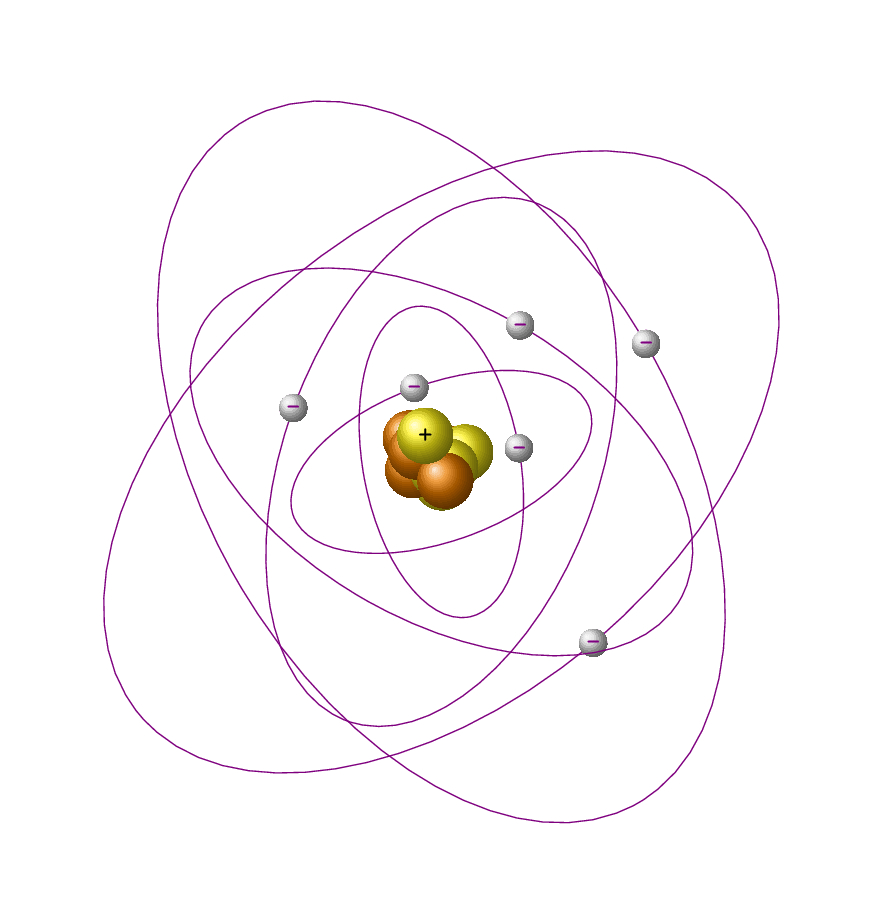
\includegraphics[width=0.6\linewidth]{atom_structure.jpeg}
\caption{原子结构模型示意图}
\label{fig:atom_structure}
\end{figure}

\textbf{电荷及其基本属性。}电荷是物质的一种基本属性，常用符号 $Q$ 或 $q$ 表示，国际单位为\textbf{库仑}（C）。一个电子所带的电量是自然界中能够独立存在的最小电荷量，称为\textbf{基本电荷} $e$：
\[
e = 1.602\,176\,634 \times 10^{-19} \ \mathrm{C}
\]
质子所带正电荷量与电子所带负电荷量大小相等、符号相反。电荷有以下三个基本性质：

\begin{enumerate}
\item \textbf{电荷守恒定律}：在一个孤立系统中，无论发生何种物理变化，正负电荷的代数和保持不变。
\item \textbf{电荷量子化}：任何带电体的电荷量只能是 $e$ 的整数倍。
\item \textbf{同性相斥、异性相吸}：同种电荷相互排斥，异种电荷相互吸引。
\end{enumerate}

\textbf{电中性。}在通常状态下，原子核内质子数与核外电子数相等，正负电荷总量相等，对外不显电性，物质呈\textbf{电中性}。当原子因外因作用（如摩擦、化学作用、光照等）得到或失去电子时，正负电荷平衡被打破，物体就带上了电。失去电子的物体带正电，得到电子的物体带负电。

\subsection{起电方式与电荷守恒}

使物体带电的过程称为\textbf{起电}。常见的起电方式有以下三种：

\textbf{(1)摩擦起电。}两种不同材料的物体相互摩擦时，由于两种原子核对价电子的束缚能力不同，束缚能力强的物体会从对方获得电子而带负电，束缚能力弱的物体则失去电子而带正电。例如丝绸与玻璃棒摩擦，玻璃棒失去电子带正电，丝绸获得电子带负电；毛皮与橡胶棒摩擦，橡胶棒带负电，毛皮带正电。摩擦起电的实质是电子通过接触面在两物体之间转移。

\textbf{(2)感应起电。}不带电的导体在带电体附近（但不接触）时，由于电荷间的同性相斥、异性相吸，导体内自由电荷会重新分布：靠近带电体的一端出现与带电体异号的电荷，远离的一端出现同号电荷。这种现象称为\textbf{静电感应}。若在感应状态下将导体瞬时接地（用手指触碰），地球这个巨大“电荷库”会与导体交换电荷，移走一端电荷；撤去接地后再移开带电体，导体就带上了与原带电体异号的电荷。整个过程\textbf{无需接触}即可使导体带电，称为\textbf{感应起电}。

\begin{figure}[H]
\centering
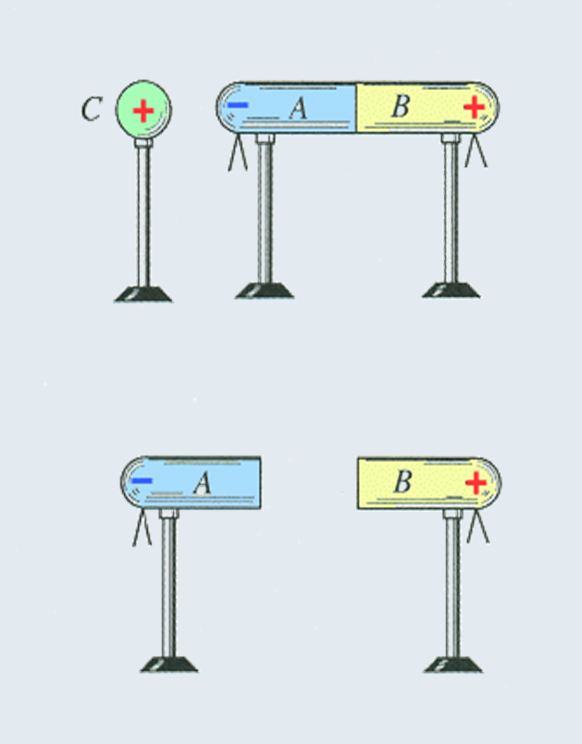
\includegraphics[width=0.5\linewidth]{induction_charging.jpeg}
\caption{感应起电原理示意图}
\label{fig:induction_charging}
\end{figure}

感应起电既有危害也有应用。例如：雷电在输电线上感应出高电压，可能击穿收音机电源变压器——故天线回路常加避雷器；而静电屏蔽（用金属罩将电路罩住）则利用感应原理使内部电路免受外界电场干扰，收音机的中频变压器外壳接地正是为此。

\textbf{(3)接触起电。}将不带电的导体与带电导体接触，部分电荷会转移到不带电导体上，使其带同种电荷。接触起电的本质是电荷在两个等位体之间重新分配，直到电位相等为止。

\textbf{电荷守恒定律。}无论何种起电方式，起电前后系统中正负电荷的代数和保持不变——摩擦起电中双方电荷等量异号，感应起电中导体两端电荷等量异号。即\textbf{电荷既不能被创造，也不能被消灭，只能从一个物体转移到另一个物体，或从物体的一部分转移到另一部分}。这就是\textbf{电荷守恒定律}，是自然界最基本的守恒定律之一，也是后文基尔霍夫电流定律的物理基础。

\textbf{静电现象与收音机。}静电荷积累在电路中常是隐患：干燥天气下人体可带上数千伏静电，触碰电路板瞬间放电，可能击穿场效应管（MOSFET）栅极氧化层。故焊接 MOS 元件时需戴接地手环、烙铁接地。本书后续讨论场效应管时将再次提到这一点。

\subsection{库仑定律与电场}

\textbf{库仑定律。}1785 年，法国物理学家库仑通过精密的扭秤实验，定量地确定了两个点电荷之间相互作用力的规律：

\begin{quote}
\textit{在真空中，两个静止点电荷之间的相互作用力 $F$，大小与它们所带电荷量 $q_1$、$q_2$ 的乘积成正比，与它们之间距离 $r$ 的平方成反比，方向沿两者的连线，同性相斥、异性相吸。}
\end{quote}

其数学表达式为
\[
F = k\frac{q_1 q_2}{r^2}
\]
式中 $k$ 为静电力常量，在真空中 $k = 9.0 \times 10^{9}\,\mathrm{N\cdot m^2/C^2}$。工程上更常用\textbf{真空介电常数} $\varepsilon_0$ 表示：
\[
k = \frac{1}{4\pi\varepsilon_0}, \qquad \varepsilon_0 \approx 8.854 \times 10^{-12}\,\mathrm{C^2/(N\cdot m^2)}
\]
在介质中，库仑定律应写为 $F = \dfrac{q_1 q_2}{4\pi\varepsilon\, r^2}$，其中 $\varepsilon$ 为介质的介电常数。

\textbf{库仑定律的意义。}库仑定律是整个静电学的定量基础，它告诉我们电荷之间存在“超距”作用力——但这一“超距”观念在十九世纪被法拉第提出的\textbf{场}的观念所取代。

\textbf{电场。}实验表明，电荷在它周围的空间产生一种特殊物质，称为\textbf{电场}。电场的基本性质是：放入电场中的任何电荷都会受到电场力的作用。借助这一观念，电荷 $q_1$ 对 $q_2$ 的作用力被理解为：$q_1$ 在空间激发电场，$q_2$ 处于该电场中而受力。电场是真实的物质存在，并非数学虚构。

\textbf{电场强度。}为定量描述电场的强弱和方向，引入\textbf{电场强度} $\mathbf{E}$（矢量）：将一检验电荷 $q_0$ 放入电场中某点，所受电场力 $\mathbf{F}$ 与 $q_0$ 之比定义为该点的电场强度：
\[
\mathbf{E} = \frac{\mathbf{F}}{q_0}
\]
电场强度的方向规定为\textbf{正电荷}在该点受力的方向，单位为\textbf{牛顿/库仑}（N/C）或\textbf{伏特/米}（V/m）。由库仑定律可推出，点电荷 $q$ 在距其 $r$ 处产生的电场强度大小为
\[
E = k\,\frac{q}{r^2}
\]

\textbf{电场线。}为形象地描绘电场，法拉第引入\textbf{电场线}（电力线）的概念：电场线从正电荷出发、到负电荷终止；曲线上每一点的切线方向即该点电场方向；电场线的疏密表示场强的大小——密则强、疏则弱。均匀电场（如两块平行带电金属板之间）的电场线是等距平行直线。

% \includegraphics{images/electric_field_lines}

\textbf{电场与电压的联系。}电场强度描述“力的分布”，而电压描述“电场力做功的本领”。设匀强电场强度为 $E$，沿电场方向相距 $d$ 的两点间电压为
\[
U = E \cdot d
\]
即电压等于电场强度与沿电场方向距离的乘积。这一关系揭示了\textbf{电压的物理本质——电场力对单位电荷做功的本领}，也为后文讨论电容器储能、天线辐射电磁波奠定了基础。

\textbf{电场与收音机。}无线电波本质上是\textbf{交变电磁场}在空间的传播——天线中的高频电流在天线周围产生交变电场和磁场，二者相互激发并向外辐射，形成电磁波。接收天线上的感应电动势则是远处电波的电场在天线导线上对自由电荷做功的结果。因此可以说，整个无线电技术都建立在"电荷—电场—电压—电流"这一物理链条之上。

\subsection{自由电子与导电}

\textbf{核外电子的分层排布。}电子在原子核外并非任意分布，而是按能量高低分层排布，由内向外依次称为 $K, L, M, N, O, P, Q$ 层。每层所能容纳的最多电子数为 $2n^2$（$n$ 为层数）。最外层的电子（\textbf{价电子}）离核较远，受核的束缚最弱，最容易受到外界影响。

\textbf{自由电子的概念。}在金属导体中，原子最外层的价电子受原子核的束缚很弱，很容易脱离单个原子的束缚，在整个金属内部作无规则的热运动。这些能够在物质内部自由移动的电子称为\textbf{自由电子}。金属内部单位体积内自由电子的数量极大，例如铜在室温下自由电子密度约为 $8.5 \times 10^{28}\,\mathrm{m^{-3}}$。

\textbf{导体、绝缘体与半导体。}根据物质内部自由电荷的多少，可将物质分为三类：

\begin{enumerate}
  \item \textbf{导体}：内部存在大量自由电荷（自由电子或离子），容易导电。常见的导体有铜、铝、银等金属，以及含离子的酸碱盐溶液。银导电性最好，铜次之，由于铜价格低廉，被广泛用作收音机电路中的导线、电感线圈和变压器绕组。
  \item \textbf{绝缘体}：几乎没有自由电荷，难以导电。如橡胶、玻璃、陶瓷、塑料、空气（干燥时）等。在收音机电路板上，绝缘基板（如环氧树脂板）用于支撑和隔离铜箔走线，防止短路。
  \item \textbf{半导体}：导电能力介于导体和绝缘体之间，且容易受温度、光照、杂质等因素影响。常见的半导体材料有硅（Si）、锗（Ge）、砷化镓（GaAs）等。矿石收音机中使用的方铅矿（PbS）晶体就是一种天然半导体；现代收音机中检波二极管、晶体管、集成电路芯片则几乎全部由硅制成。
\end{enumerate}

% \includegraphics{images/conductor_insulator}

\textbf{半导体的特殊意义。}半导体之所以成为整个电子工业的基础，在于其导电能力可通过掺入微量杂质而被精确控制——这正是制造二极管、晶体管和集成电路的关键。从某种意义上说，整个收音机发展史就是从"天然半导体"（矿石晶体）到"人工半导体"（晶体管、集成电路）的演进史。

\subsection{电流的形成}

\textbf{电流的定义。}电荷的\textbf{定向移动}就形成了电流。需要强调的是：并非任何电荷运动都形成电流——只有电荷在宏观上出现\textbf{定向}移动时，才称为电流。例如金属导体中自由电子时刻在做无规则热运动，但整体上向各方向运动的机会均等，并不会形成电流；只有当外加电压迫使电子向某一方向定向漂移时，才形成电流。

\textbf{产生电流的条件。}要在导体中维持持续的电流，必须同时满足两个条件：
\begin{enumerate}
  \item 导体内部存在可以自由移动的电荷（自由电子或离子）；
  \item 导体两端存在一定的\textbf{电压}（电位差），以驱动电荷定向移动。
\end{enumerate}

提供电压的装置称为\textbf{电源}，如电池、发电机等。电源通过非静电力（如化学力、电磁力）将正负电荷分离，使电源两极维持一定的电位差。

\textbf{电流的方向。}历史上，人们规定\textbf{正电荷定向移动的方向}为电流方向。这一规定是在发现电子之前作出的，但沿用至今。在金属导体中实际移动的是带负电的自由电子，因此金属导体中的\textbf{电子流方向}与规定的电流方向相反。这一点在分析收音机电路时尤需注意：电路图上标出的电流方向（箭头）指的是\textbf{习惯电流方向}，而电子实际流动方向与之相反。

% \includegraphics{images/current_direction}

\textbf{电流的连续性。}在闭合电路中，电流是连续不断的：在电源外部，电流从电源正极出发，经导线和负载回到负极；在电源内部，依靠电源的非静电力将电荷从负极搬运到正极，从而维持电流持续流动。整个回路上电流处处相等，没有电荷的积累或消失——这就是后面将要学习的\textbf{基尔霍夫电流定律}的物理基础。

\textbf{从电流到信号。}在收音机电路中，我们关心的电流不仅有大小，还有随时间变化的规律。声音信号经过话筒转换为与之对应的\textbf{变化电流}，经放大、调制后由天线辐射出去；接收端天线捕捉到无线电波后再次产生\textbf{感应电流}，经放大和解调最终还原为声音。可以说，整个无线电技术就是关于"如何产生、控制、传输和检测电流"的学问。

\section{电流、电压与电阻}
\label{sec:current_voltage_resistance}

\subsection{电流}

\textbf{电流的大小。}电流的强弱用\textbf{电流}（这一物理量与现象同名）来描述，符号为 $I$ 或 $i$。其定义为：通过导体横截面的电荷量 $q$ 与所用时间 $t$ 之比，即
\[
I = \frac{q}{t}
\]
在导体中，若在 $1$ 秒内通过某横截面的电荷量为 $1$ 库仑，则该处的电流为 $1$ \textbf{安培}（A）。电流的国际单位是安培（A），常用的辅助单位还有千安（kA）、毫安（mA）、微安（$\mu$A）等：
\[
1\,\mathrm{A} = 10^{3}\,\mathrm{mA} = 10^{6}\,\mu\mathrm{A}
\]

\textbf{电流的方向。}如前所述，习惯上规定正电荷定向移动的方向为电流方向。在金属导体中，电流方向与电子流方向相反。

\textbf{恒定电流与变化电流。}大小和方向都不随时间变化的电流称为\textbf{恒定电流}（直流电，DC），例如干电池、蓄电池所提供的电流；大小或方向随时间变化的电流称为\textbf{变化电流}，其中按正弦规律周期性变化的称为\textbf{交流电}（AC），如家用 $220\,\mathrm{V}$ 电源。在收音机电路中，既有直流（电源供电）又有交流（信号、本振、中频等），分析时需要加以区分。

\textbf{电流密度。}在截面不同的导体中，仅看总电流大小并不能反映导体内电荷分布情况。为此引入\textbf{电流密度} $J$，定义为单位横截面上通过的电流：
\[
J = \frac{I}{S}
\]
其单位为 $\mathrm{A/m^2}$。电流密度是计算导线安全载流量、线圈发热等问题的重要参数。例如绕制收音机天线线圈时，通过漆包线的电流密度不能过大，否则线圈发热严重，效率降低。

\textbf{参考方向。}在分析较复杂的电路时，电流的真实方向往往事先难以判断。这时可任意假定一个方向作为\textbf{参考方向}，并在电路图上用箭头标出。若按此方向计算出的电流为正值，说明实际方向与参考方向相同；若为负值，则实际方向与参考方向相反。这一方法在后述电路分析中将被反复使用。

\textbf{关联参考方向。}对一个二端元件而言，电流的参考方向和电压的参考极性都可以任意设定。但为统一起见，工程上常采用\textbf{关联参考方向}：让电流的参考方向从电压参考极性的"$+$"端流入、从"$-$"端流出，如图所示。采用关联参考方向后，功率 $P = UI$ 的符号有明确的物理意义：
\begin{itemize}
  \item $P > 0$：元件\textbf{吸收}功率（消耗电能），是\textbf{负载}；
  \item $P < 0$：元件\textbf{发出}功率（提供电能），是\textbf{电源}。
\end{itemize}
若采用非关联参考方向，则判断规则相反。本书后续电路分析中默认采用关联参考方向，仅在必要时另作说明。

% \includegraphics{images/passive_sign_convention}

\textbf{参考方向的意义。}参考方向是电路分析中一个看似简单却极为重要的概念。它把"方向未知"的物理量转化为"代数符号可定"的数学量，使电路方程的列写和求解有了一套严谨的规则。读者务必从一开始就养成"先标参考方向、再列方程"的习惯。

\subsection{电压与电动势}

\textbf{电位的概念。}电场中某点的\textbf{电位}（电势）在数值上等于把单位正电荷从该点移动到参考点（无穷远或大地）时电场力所做的功。参考点的电位规定为零，工程上常以\textbf{大地}或\textbf{电源负极}作为零电位参考点。电位是相对量，其数值随参考点的选取而变。

\textbf{电压。}\textbf{电压}（又称\textbf{电位差}）是电场中两点之间的电位之差，表示电场力把单位正电荷从一点移动到另一点所做的功。设 $a$ 点电位为 $V_a$，$b$ 点电位为 $V_b$，则 $a$、$b$ 两点间的电压为
\[
U_{ab} = V_a - V_b
\]
电压的国际单位是\textbf{伏特}（V），常用辅助单位有千伏（kV）、毫伏（mV）、微伏（$\mu$V）等。$1\,\mathrm{V}=10^3\,\mathrm{mV}=10^6\,\mu\mathrm{V}$。

\textbf{电压的方向。}电压的方向规定为由高电位指向低电位，即电位降低的方向。在电路图中，电压方向常用箭头或"$+$、$-$"极性表示。同样，分析中也可任意设定\textbf{参考极性}，计算结果为正表示实际极性与参考极性一致，为负则相反。

\textbf{电动势。}\textbf{电动势}（EMF）反映电源将其他形式能量转换为电能的本领，定义为：电源内部非静电力把单位正电荷从负极搬运到正极所做的功，符号为 $E$ 或 $\varepsilon$，单位也是伏特（V）。电动势的方向规定为：在电源内部由负极指向正极，即电位升高的方向，与电源外部电流方向一致。

\textbf{电动势与电压的区别。}两者虽然单位相同，但物理含义不同：
\begin{itemize}
  \item \textbf{电动势}描述的是\textbf{电源}通过非静电力做功的本领，对应"电位升高"；
  \item \textbf{电压}描述的是电场力做功的本领，对应"电位降低"。
\end{itemize}
对于实际电源，由于存在\textbf{内阻} $r$，当电源对外输出电流 $I$ 时，端电压与电动势的关系为
\[
U = E - I\,r
\]
可见，输出电流越大，端电压越低。这一现象在收音机使用电池供电时尤为明显：电池用久后内阻增大，开机时电压急剧下降，导致收音机声音变小或不能正常工作。

\textbf{接地与参考点。}工程上把电路中选作零电位的参考点称为\textbf{"地"}（ground），把电路某点与该参考点相连接称为\textbf{接地}。这里必须区分两种不同含义的"地"：
\begin{itemize}
  \item \textbf{电路地}（参考地、信号地）：仅为分析方便而选定的零电位基准，可以是电源负极或一条公共导线（俗称"地线"或"公共母线"），\textbf{不一定}与大地相连。它是电路图中各处电压标注的隐含参考点。
  \item \textbf{大地地}（保护地）：通过接地极真正接入大地，主要用于人身安全和设备保护——一旦绝缘损坏使机壳带电，故障电流可经大地泄放，使保护装置动作。
\end{itemize}
在收音机等便携式电子设备中，通常以电源负极或机内金属底板作为公共"地"，电路图中各点电压均相对此点测量。接地在电路图中有专门的图形符号：一般接地用一组逐渐变短的平行横线表示，保护接地则另用专门的符号加以区分。合理的接地不仅能统一电位基准，更是抑制噪声、保证电路稳定工作的基础——这一问题的工程细节将在第\ref{chap:soldering_basics}章焊接与装配中进一步讨论。

\subsection{电阻}

\textbf{电阻的定义。}电流通过导体时会受到阻碍作用，导体对电流的阻碍程度称为\textbf{电阻}，符号为 $R$ 或 $r$。电阻的国际单位是\textbf{欧姆}（$\Omega$），辅助单位有千欧（k$\Omega$）、兆欧（M$\Omega$）等：
\[
1\,\mathrm{k\Omega} = 10^3\,\Omega, \quad 1\,\mathrm{M\Omega} = 10^6\,\Omega
\]

\textbf{电阻定律。}在温度一定时，一段均匀导体的电阻与其长度 $l$ 成正比，与横截面积 $S$ 成反比，即
\[
R = \rho \, \frac{l}{S}
\]
式中比例系数 $\rho$ 称为\textbf{电阻率}，单位为 $\Omega\cdot\mathrm{m}$。电阻率反映材料本身的导电性能：$\rho$ 越小，导电性能越好。下表列出常见材料在 $20^{\circ}\mathrm{C}$ 时的电阻率：

\begin{center}
\begin{tabular}{lc}
\hline
\textbf{材料} & \textbf{电阻率 $\rho$ ($\Omega\cdot$m)} \\
\hline
银 & $1.65 \times 10^{-8}$ \\
铜 & $1.75 \times 10^{-8}$ \\
铝 & $2.83 \times 10^{-8}$ \\
钨 & $5.3 \times 10^{-8}$ \\
铁 & $9.78 \times 10^{-8}$ \\
碳 & $3.5 \times 10^{-5}$ \\
锗 & $\approx 0.6$ \\
硅 & $\approx 2.3 \times 10^{3}$ \\
\hline
\end{tabular}
\end{center}

可见金属导体电阻率极小，而纯净半导体电阻率却很大——这正是通过\textbf{掺杂}能极大改变其导电性能的原因。

\textbf{温度对电阻的影响。}导体的电阻还与温度有关。\textbf{金属导体}的电阻随温度升高而\textbf{增大}；某些\textbf{合金}（如锰铜、康铜）的电阻几乎不随温度变化，常用作标准电阻；而\textbf{半导体}的电阻则随温度升高而\textbf{急剧减小}，利用这一特性可制成\textbf{热敏电阻}，用于温度测量和补偿。温度对电阻的影响用\textbf{电阻温度系数} $\alpha$ 来描述：
\[
R_t = R_0 \big[1 + \alpha (t - t_0)\big]
\]
式中 $R_t$、$R_0$ 分别为温度 $t$、$t_0$ 时的电阻值。

\textbf{电阻的物理本质。}从微观角度看，电阻来源于自由电子在运动中与晶格离子发生碰撞所造成的能量损耗。碰撞越频繁，电阻越大；温度升高使晶格热振动加剧，碰撞频率增大，因此金属电阻随温度升高而增大。

\textbf{电导。}电阻的倒数称为\textbf{电导}，用 $G$ 表示：
\[
G = \frac{1}{R}
\]
电导反映导体\textbf{导电}的能力，单位为\textbf{西门子}（S），$1\,\mathrm{S} = 1\,\Omega^{-1}$。电导 $G$ 与电导率 $\sigma$（电阻率 $\rho$ 的倒数，$\sigma = 1/\rho$）的关系为
\[
G = \sigma \cdot \frac{S}{l}
\]
在分析并联电路时，使用电导往往比电阻更方便——并联总电导等于各支路电导之和：
\[
G = G_1 + G_2 + \cdots + G_n
\]
这与串联电阻的求和形式完全对偶。后续学习节点电压法时，电导形式将使方程更简洁。

\textbf{电阻在收音机电路中的作用。}电阻是收音机电路中使用最多的元件之一，主要用于：限制电流（如晶体管偏置电阻）、分压（如音量电位器）、负载（如检波器负载电阻）、滤波（与电容组成RC滤波）等。理解电阻的性质对分析任何电子电路都是基础中的基础。

\subsection{电源与电池}

\textbf{电源的作用。}电源是把其他形式能量转换为电能的装置，其作用是维持电源两极一定的电位差（电动势），从而在闭合电路中形成持续的电流。电源按其输出电流的性质分为\textbf{直流电源}（如干电池、蓄电池、直流稳压电源）和\textbf{交流电源}（如市电、信号发生器）。本节主要讨论直流电源。

\textbf{理想电源与实际电源。}为分析方便，常引入两类理想电源模型：
\begin{itemize}
  \item \textbf{理想电压源}：端电压恒定，不随输出电流变化，内阻为零；
  \item \textbf{理想电流源}：输出电流恒定，不随端电压变化，内阻为无穷大。
\end{itemize}
实际电源都存在一定内阻 $r$，端电压随输出电流增大而下降（$U = E - Ir$）。故实际电源可视为\textbf{理想电压源 $E$ 串联内阻 $r$}（这称为实际电源的\textbf{电压源模型}），也可等效为\textbf{理想电流源 $I_S = E/r$ 并联内阻 $r$}（\textbf{电流源模型}）。两种模型可通过\textbf{电源等效变换}相互转换，这一方法在 §1.3 中将进一步讨论。

\textbf{电源的串联。}将多个电源\textbf{正负极依次相接}的连接方式称为串联。串联电源的特点：
\begin{itemize}
  \item 总电动势等于各电源电动势的\textbf{代数和}（同向串联为正，反向串联为负）：
  \[
  E = E_1 + E_2 + \cdots + E_n
  \]
  \item 总内阻等于各电源内阻之和：$r = r_1 + r_2 + \cdots + r_n$；
  \item 通过各电源的电流相等。
\end{itemize}
\textbf{应用：}当单个电池电压不足以驱动电路时，常将多节电池串联以提高电压。例如：早期电子管收音机甲电（灯丝电源）常用两节 $1.5\,\mathrm{V}$ 干电池串联得 $3\,\mathrm{V}$；便携式晶体管收音机常用 $6\,\mathrm{F22}$ 型 $9\,\mathrm{V}$ 叠层电池（内部由 $6$ 节 $1.5\,\mathrm{V}$ 电池串联）。但需注意：串联电池组中若某一节电池反向（接反或失效），将抵消其他电池的电动势并可能引起漏液。

\textbf{电源的并联。}将多个电源\textbf{同极性端分别接在一起}的连接方式称为并联。并联电源的特点：
\begin{itemize}
  \item 总电动势等于单个电源电动势（要求并联的各电源电动势\textbf{相同}）；
  \item 总内阻等于各电源内阻并联后的等效值：
  \[
  r = \frac{r_1 \parallel r_2 \parallel \cdots \parallel r_n}{\text{（并联）}}
  \]
  \item 总输出电流等于各电源输出电流之和。
\end{itemize}
\textbf{应用：}并联不能提高电压，但能\textbf{增大输出电流能力}并\textbf{减小等效内阻}，常用于需要大电流或延长供电时间的场合。例如便携式收音机为延长使用时间，常将两节电池并联供电。

\textbf{注意事项。}并联电池必须是\textbf{同型号、同电压、同新旧程度}的电池，否则电压高的电池会向电压低的电池\textbf{充电}，引起发热、漏液甚至爆炸。这是初学者常犯的错误。

\textbf{常见电池类型。}收音机常用的电池有以下几种：

\begin{center}
\begin{tabular}{lccp{6.5cm}}
\hline
\textbf{类型} & \textbf{电压} & \textbf{可充电} & \textbf{特点与用途} \\
\hline
锌锰干电池 & $1.5\,\mathrm{V}$ & 否 & 价格低，内阻较大；适合小电流间歇工作，普通便携收音机用 \\
碱性电池 & $1.5\,\mathrm{V}$ & 否 & 容量大、内阻小、低温性能好；适合较大电流设备 \\
叠层电池 & $9\,\mathrm{V},\,12\,\mathrm{V}$ 等 & 否 & 体积小、电压高、容量小；用于便携式收音机、万用表 \\
铅酸蓄电池 & $2.0\,\mathrm{V}$/单体 & 是 & 容量大、可大电流放电；早期电子管收音机甲、乙电源常用 \\
镍镉电池 & $1.2\,\mathrm{V}$ & 是 & 内阻极小、可大电流放电、有记忆效应；早期对讲机用 \\
镍氢电池 & $1.2\,\mathrm{V}$ & 是 & 容量大、无重金属污染；中高端便携设备用 \\
锂离子电池 & $3.7\,\mathrm{V}$ & 是 & 能量密度高、自放电小；现代数字收音机、SDR 用 \\
\hline
\end{tabular}
\end{center}

\textbf{电池内阻对收音机的影响。}电池内阻随使用时间增大、随温度降低而增大。当收音机开机瞬间功率放大管需要较大电流时，电池内阻压降增大使端电压急剧下跌，可能导致：
\begin{itemize}
  \item 收音机声音变小、失真、低端电台收不到；
  \item 微处理器控制的数字收音机自动关机或复位；
  \item 电池发热严重。
\end{itemize}
判断电池是否内阻过大，可在带载情况下测量端电压：若空载电压正常但带载后电压大幅下降，说明电池内阻已增大，应及时更换。这是收音机维修中最常见的"故障"之一。

\section{欧姆定律与电路基本定律}
\label{sec:ohm_law}

\subsection{欧姆定律}

\textbf{部分电路欧姆定律。}德国物理学家欧姆通过大量实验于 $1826$ 年总结出：通过一段导体的电流 $I$ 与这段导体两端的电压 $U$ 成正比，与这段导体的电阻 $R$ 成反比，即
\[
\boxed{\,I = \frac{U}{R}\,}
\]
式中 $U$ 的单位为伏特（V），$R$ 的单位为欧姆（$\Omega$），$I$ 的单位为安培（A）。该式称为\textbf{部分电路欧姆定律}。它也可改写为
\[
U = I \cdot R, \qquad R = \frac{U}{I}
\]

\textbf{使用注意事项。}
\begin{enumerate}
  \item 公式中的 $U$、$I$、$R$ 必须对应\textbf{同一段电路}，不能张冠李戴；
  \item 公式只适用于\textbf{线性电阻}（电压电流关系为直线的电阻）；
  \item 必须注意\textbf{单位}：当电压用 V、电流用 A 时，电阻才是 $\Omega$。
\end{enumerate}

\textbf{全电路欧姆定律。}包含电源在内的闭合电路称为\textbf{全电路}。在全电路中，电流 $I$ 等于电源电动势 $E$ 与外电路总电阻 $R$ 加电源内阻 $r$ 之比：
\[
I = \frac{E}{R + r}
\]
相应地，外电路两端电压（端电压）为 $U = IR = E - Ir$。当外电路断开时（$I=0$），端电压等于电动势；当外电路短路时（$R=0$），$I = E/r$，由于内阻 $r$ 通常很小，短路电流可能很大，烧毁电源。

% \includegraphics{images/full_circuit_ohm}

\textbf{线性电阻与非线性电阻。}
\begin{itemize}
  \item \textbf{线性电阻}：电压—电流关系是一条过原点的直线，电阻值不随电压、电流变化。一般的金属膜电阻、碳膜电阻在正常工作范围内都可视为线性电阻。
  \item \textbf{非线性电阻}：电压—电流关系不是直线，电阻值随工作点变化。典型的非线性电阻有\textbf{二极管}、\textbf{热敏电阻}、\textbf{白炽灯灯丝}等。例如收音机中的检波二极管，正向导通时两端电压基本稳定在 $0.2\sim0.7\,\mathrm{V}$，并不遵循欧姆定律。
\end{itemize}

\textbf{欧姆定律在收音机电路中的应用。}欧姆定律是分析收音机电路最基本、最常用的工具。例如：已知晶体管发射极电阻 $R_e = 1\,\mathrm{k\Omega}$，测得两端电压 $U_e = 2\,\mathrm{V}$，则发射极电流
\[
I_e = \frac{U_e}{R_e} = \frac{2\,\mathrm{V}}{1000\,\Omega} = 2\,\mathrm{mA}
\]
从而可推算晶体管的工作状态（这一过程在收音机调试与故障检修中极为常用）。

\textbf{电压源模型与电流源模型的等效变换。}实际电源既可用"\textbf{理想电压源 $E$ 串联内阻 $r$}"表示（电压源模型），也可用"\textbf{理想电流源 $I_S$ 并联内阻 $r$}"表示（电流源模型），如图所示。两种模型对外电路的效果完全相同，可相互等效变换。

% \includegraphics{images/source_transform}

\textbf{等效变换公式：}
\[
I_S = \frac{E}{r}, \qquad E = I_S \cdot r
\]
等效变换时\textbf{内阻 $r$ 不变}，仅改变电源形式。需要注意：
\begin{itemize}
  \item \textbf{电压源}（$E$ 与 $r$ 串联）变换为\textbf{电流源}（$I_S$ 与 $r$ 并联）时，电流源方向应与电压源由负极指向正极的方向一致；
  \item \textbf{电流源}变换为\textbf{电压源}时，电压源正极在电流源流出端；
  \item \textbf{理想电压源}（$r=0$）与\textbf{理想电流源}（$r=\infty$）之间\textbf{不能}等效变换；
  \item 与理想电压源并联的元件对外电路无影响（可断开），与理想电流源串联的元件对外电路无影响（可短路）——这是简化电路的常用技巧。
\end{itemize}

\textbf{应用举例。}利用电源等效变换，可将复杂电路逐步化简为单回路电路。这一方法在分析多电源供电网络、晶体管放大器等效电路时极为方便。它与后文的戴维南定理、诺顿定理一脉相承，本质上都是"寻找最简等效电路"的思想。

\subsection{基尔霍夫定律}

欧姆定律只能分析简单电路。对于多电源、多回路的复杂电路，必须借助\textbf{基尔霍夫定律}（KCL、KVL）。它是 $1845$ 年由德国物理学家基尔霍夫提出的，是电路分析的基石。

在介绍定律之前，先定义几个常用术语：
\begin{itemize}
  \item \textbf{支路}：电路中通过同一电流的每一段路径；
  \item \textbf{节点}：三条或三条以上支路的连接点；
  \item \textbf{回路}：电路中任一闭合路径；
  \item \textbf{网孔}：内部不再含有其他支路的回路，即"最小回路"。
\end{itemize}

\textbf{基尔霍夫电流定律（KCL）。}\textbf{KCL}的内容是：在任一时刻，流入某一节点的电流之和等于流出该节点的电流之和；或者说，节点上电流的代数和恒为零：
\[
\sum I_{\text{入}} = \sum I_{\text{出}} \qquad \text{或} \qquad \sum I = 0
\]
KCL 的物理本质是\textbf{电荷守恒定律}——节点上不能有电荷的积累或消失。

% \includegraphics{images/kcl_kvl}

\textbf{基尔霍夫电压定律（KVL）。}\textbf{KVL}的内容是：在任一时刻，沿任一闭合回路绕行一周，各段电压的代数和恒为零：
\[
\sum U = 0
\]
或写作：回路中电动势的代数和等于各电阻上电压降的代数和。KVL 的物理本质是\textbf{能量守恒定律}——电荷沿回路绕行一周回到原点，电位不变，所做的总功为零。

\textbf{符号规定。}应用 KCL 时，常规定流入节点的电流为正，流出为负（或反之）；应用 KVL 时，先任意选定\textbf{绕行方向}，凡电压方向与绕行方向相同者取正，相反者取负；电动势方向（电源内部由负到正）与绕行方向一致时取正，否则取负。

\textbf{支路电流法。}利用基尔霍夫定律求解复杂电路的步骤为：
\begin{enumerate}
  \item 标定各支路电流的参考方向；
  \item 对节点列 KCL 方程（若有 $n$ 个节点，可列 $n-1$ 个独立方程）；
  \item 对网孔列 KVL 方程（若有 $m$ 个支路，则可列 $m - (n-1)$ 个独立网孔方程）；
  \item 联立求解，得到各支路电流；
  \item 由所得电流的正负判断实际方向。
\end{enumerate}

\textbf{示例。}如图电路中，$E_1=3\,\mathrm{V}$，$E_2=6\,\mathrm{V}$，$R_1=1\,\Omega$，$R_2=2\,\Omega$，$R_3=3\,\Omega$，求通过 $R_3$ 的电流。

设三条支路电流 $I_1$、$I_2$、$I_3$ 方向如图，节点 $A$ 的 KCL 方程为：
\[
I_1 + I_2 = I_3
\]
两个网孔的 KVL 方程为：
\[
E_1 - I_1 R_1 - I_3 R_3 = 0, \qquad -E_2 - I_2 R_2 - I_3 R_3 = 0
\]
注意第二个网孔绕行方向上 $E_2$ 为反向（电动势方向与绕行方向相反），故取负号。代入数据：
\[
3 - I_1 - 3 I_3 = 0 \Rightarrow I_1 = 3 - 3 I_3
\]
\[
-6 - 2 I_2 - 3 I_3 = 0 \Rightarrow I_2 = -3 - \tfrac{3}{2} I_3
\]
代入 KCL 方程 $I_1 + I_2 = I_3$：
\[
(3 - 3 I_3) + \left(-3 - \tfrac{3}{2} I_3\right) = I_3
\]
\[
-\tfrac{9}{2} I_3 = 0 \Rightarrow I_3 = 0\,\mathrm{A}
\]
进一步得 $I_1 = 3\,\mathrm{A}$，$I_2 = -3\,\mathrm{A}$（负号说明 $I_2$ 实际方向与参考方向相反）。

\textbf{结果讨论。}本题中两电源电动势 $E_1$、$E_2$ 经电阻 $R_1$、$R_2$ 分压后恰好在节点 $A$ 处电位相等，故 $R_3$ 上无电流。这是一个值得细品的特例：当两个含源支路在公共节点处电位相等时，连接它们的第三支路无电流——这一结论在分析晶体管推挽电路、平衡电桥等场合很有用。

\textbf{支路电流法的特点。}这种"列方程—代数求解"的方法虽显繁琐，但通用性极强，是分析晶体管收音机偏置电路、推挽输出电路的基础。对节点数、网孔数较多的大电路，手工求解繁琐，可借助计算机电路仿真软件（如 SPICE）求解。

\subsection{网孔电流法与节点电压法}

支路电流法虽然通用，但当支路数较多时方程数也多，求解繁琐。\textbf{网孔电流法}和\textbf{节点电压法}是两种最常用的简化方法，它们通过减少未知量个数来减少方程数，是工程电路分析的标准方法。

\textbf{网孔电流法。}\textbf{网孔电流法}以\textbf{网孔电流}（假想沿每个网孔边界流动的电流）为未知量，对每个网孔列 KVL 方程。设电路有 $m$ 个网孔，则只需列 $m$ 个方程（比支路电流法的 $2m-1$ 个方程少一半左右）。

\textbf{求解步骤：}
\begin{enumerate}
  \item 为每个网孔任意设定一个\textbf{网孔电流}参考方向（通常统一取顺时针或逆时针）；
  \item 对每个网孔列 KVL 方程：沿网孔电流方向绕行一周，$\sum E = \sum I R$；
  \item 求解方程组得各网孔电流；
  \item 由网孔电流推算各支路电流——\textbf{单独属于某网孔的支路}，支路电流等于该网孔电流；\textbf{两网孔公共支路}，支路电流等于两网孔电流的代数和。
\end{enumerate}

\textbf{网孔电流法示例。}仍以前述 $E_1=3\,\mathrm{V}$，$E_2=6\,\mathrm{V}$，$R_1=1\,\Omega$，$R_2=2\,\Omega$，$R_3=3\,\Omega$ 电路为例。设左网孔电流 $I_a$（顺时针）、右网孔电流 $I_b$（逆时针），二者在 $R_3$ 上方向相反。则
\[
\begin{cases}
E_1 = I_a R_1 + (I_a - I_b) R_3 \\
-E_2 = I_b R_2 + (I_b - I_a) R_3
\end{cases}
\quad\Rightarrow\quad
\begin{cases}
3 = I_a + 3(I_a - I_b) \\
-6 = 2 I_b + 3(I_b - I_a)
\end{cases}
\]
整理后联立求解，得 $I_a = 3\,\mathrm{A}$，$I_b = 3\,\mathrm{A}$。$R_3$ 上电流 $I_3 = I_a - I_b = 0\,\mathrm{A}$，结果与支路电流法完全一致，而方程数量减半。

\textbf{节点电压法。}\textbf{节点电压法}以\textbf{节点电压}（各节点相对于参考点的电位）为未知量，对每个独立节点列 KCL 方程。设电路有 $n$ 个节点，选其中一个为参考点（零电位），则只需对剩余 $n-1$ 个节点列方程。

\textbf{求解步骤：}
\begin{enumerate}
  \item 选定参考节点（通常选电源负极或元件汇集最多处），其余节点电位 $V_1$、$V_2$、$\cdots$ 为未知量；
  \item 用节点电压表示各支路电流（如 $I_k = (V_a - V_b)/R_k$ 或 $I_k = (V_a - V_b + E)/R_k$）；
  \item 对每个独立节点列 KCL 方程 $\sum I_{\text{出}} = 0$；
  \item 求解方程组得各节点电压，再由节点电压求各支路电流。
\end{enumerate}

\textbf{节点电压法的特点。}当电路中节点数少于网孔数时（例如多支路汇聚于少数节点），节点电压法尤为简便。它也是 SPICE 等电路仿真软件内部采用的主要分析方法。在收音机电路中，分析多级放大器的级间耦合、电源分配网络时常采用此法。

\textbf{两种方法的选择。}一般而言：
\begin{itemize}
  \item \textbf{网孔数 < 节点数 - 1}：选用网孔电流法；
  \item \textbf{节点数 - 1 < 网孔数}：选用节点电压法；
  \item 含\textbf{理想电压源}支路较多时：节点电压法更方便（电压源支路节点电压已知）；
  \item 含\textbf{理想电流源}支路较多时：网孔电流法更方便（电流源所在网孔电流已知）。
\end{itemize}

\textbf{与支路电流法的对比。}三种方法本质都是基尔霍夫定律的应用，区别仅在于选取的未知量不同。建议读者在初学阶段同时使用三种方法求解同一电路，对比结果与计算量，加深对电路分析思想的理解。

\subsection{串并联电路}

\textbf{电阻的串联。}将若干电阻\textbf{首尾相接}，流过同一电流的连接方式称为串联。串联电路具有以下特点：
\begin{enumerate}
  \item 通过各电阻的电流\textbf{相等}：$I = I_1 = I_2 = \cdots = I_n$；
  \item 总电压等于各电阻上电压之和：$U = U_1 + U_2 + \cdots + U_n$；
  \item \textbf{等效电阻}（总电阻）等于各电阻之和：
  \[
  R = R_1 + R_2 + \cdots + R_n
  \]
  \item 各电阻上的电压与电阻成正比分配（\textbf{分压原理}）：
  \[
  U_1 : U_2 : \cdots : U_n = R_1 : R_2 : \cdots : R_n
  \]
\end{enumerate}
两个电阻串联时：$U_1 = \dfrac{R_1}{R_1 + R_2} U$，$U_2 = \dfrac{R_2}{R_1 + R_2} U$。

\textbf{电阻的并联。}将若干电阻\textbf{两端分别接在一起}，使各电阻承受同一电压的连接方式称为并联。并联电路具有以下特点：
\begin{enumerate}
  \item 各电阻两端电压\textbf{相等}：$U = U_1 = U_2 = \cdots = U_n$；
  \item 总电流等于各电阻上电流之和：$I = I_1 + I_2 + \cdots + I_n$；
  \item \textbf{等效电阻的倒数}等于各电阻倒数之和：
  \[
  \frac{1}{R} = \frac{1}{R_1} + \frac{1}{R_2} + \cdots + \frac{1}{R_n}
  \]
  \item 各电阻上的电流与电阻成反比分配（\textbf{分流原理}）：
  \[
  I_1 : I_2 : \cdots : I_n = \frac{1}{R_1} : \frac{1}{R_2} : \cdots : \frac{1}{R_n}
  \]
\end{enumerate}
两个电阻并联时，等效电阻为
\[
R = \frac{R_1 R_2}{R_1 + R_2}
\]
对应的分流公式：
\[
I_1 = \frac{R_2}{R_1 + R_2} I, \qquad I_2 = \frac{R_1}{R_1 + R_2} I
\]

\textbf{串并联的直观规律。}
\begin{itemize}
  \item 串联总电阻\textbf{大于}其中任何一个电阻；
  \item 并联总电阻\textbf{小于}其中任何一个电阻；
  \item 若两个相等电阻并联，总电阻减半；$n$ 个相等电阻并联，总电阻为单个的 $1/n$。
\end{itemize}

\textbf{分压与分流在收音机中的应用。}
\begin{itemize}
  \item \textbf{音量电位器}：本质上是一个串联分压电路，滑动触点改变两部分电阻的比例，从而改变输出电压，达到调节音量的目的。
  \item \textbf{电压表扩大量程}：在表头串联大电阻（分压），可测量较高电压。
  \item \textbf{电流表扩大量程}：在表头并联小电阻（分流），可测量较大电流。
  \item \textbf{晶体管发射极电阻并联旁路电容}：对直流而言是串联限流；对交流信号而言，电容视为短路，使发射极电阻被"交流旁路"，避免交流负反馈——这是晶体管收音机中极为常见的电路形式。
\end{itemize}

\textbf{混联电路。}实际电路中常是串联与并联组合的\textbf{混联电路}。分析时一般采用"\textbf{逐步化简法}"：从最远离电源端的支路开始，按串、并联规律依次合并，求出等效总电阻，再回到原电路逐段求电压电流。

\textbf{Y-$\triangle$ 变换。}某些电路中，三个电阻既非串联也非并联，而是接成\textbf{星形}（Y 形）或\textbf{三角形}（$\triangle$ 形）结构，无法用串并联直接化简。此时可用\textbf{Y-$\triangle$ 等效变换}将两种结构相互转换，使电路化简成为可能。

% \includegraphics{images/y_delta_transform}

\textbf{Y 形 $\to$ $\triangle$ 形}（已知 Y 形三电阻 $R_1, R_2, R_3$，求 $\triangle$ 形三电阻 $R_{12}, R_{23}, R_{31}$）：
\[
R_{12} = \frac{R_1 R_2 + R_2 R_3 + R_3 R_1}{R_3}, \quad
R_{23} = \frac{R_1 R_2 + R_2 R_3 + R_3 R_1}{R_1}, \quad
R_{31} = \frac{R_1 R_2 + R_2 R_3 + R_3 R_1}{R_2}
\]

\textbf{$\triangle$ 形 $\to$ Y 形}（已知 $\triangle$ 形三电阻，求 Y 形三电阻）：
\[
R_1 = \frac{R_{12} R_{31}}{R_{12} + R_{23} + R_{31}}, \quad
R_2 = \frac{R_{12} R_{23}}{R_{12} + R_{23} + R_{31}}, \quad
R_3 = \frac{R_{23} R_{31}}{R_{12} + R_{23} + R_{31}}
\]

\textbf{对称情形。}若 Y 形三个电阻相等（$R_1 = R_2 = R_3 = R_Y$），则变换后 $\triangle$ 形三个电阻也相等，且
\[
R_\triangle = 3 R_Y
\]
反之 $R_Y = R_\triangle / 3$。

\textbf{应用。}经典的\textbf{惠斯通电桥}（用于精确测量电阻）在\textbf{不平衡}状态下，桥路中五个电阻即构成 Y 形或 $\triangle$ 形结构，必须借助 Y-$\triangle$ 变换才能化简。晶体管收音机的某些衰减网络、匹配网络也采用 Y 形或 $\triangle$ 形结构。掌握这一变换，是分析复杂电阻网络的有力工具。

\subsection{受控源与含受控源电路分析}

\textbf{独立源与受控源。}前面遇到的电压源、电流源，其电动势或电流值是\textbf{独立给定}的，不受电路中其他变量影响，称为\textbf{独立源}。而在电子电路中，许多器件的输出受电路中某一电压或电流控制——这种"电源"称为\textbf{受控源}（又称\textbf{非独立源}）。

\textbf{受控源的四种类型。}按控制量（电压或电流）和被控量（电压或电流）的不同组合，受控源分为四种：

\begin{center}
\begin{tabular}{llll}
\hline
\textbf{类型} & \textbf{符号} & \textbf{控制量} & \textbf{被控量} \\
\hline
电压控制电压源（VCVS） & $\mu U_1$ & 电压 $U_1$ & 电压 $\mu U_1$ \\
电压控制电流源（VCCS） & $g U_1$ & 电压 $U_1$ & 电流 $g U_1$ \\
电流控制电压源（CCVS） & $r I_1$ & 电流 $I_1$ & 电压 $r I_1$ \\
电流控制电流源（CCCS） & $\beta I_1$ & 电流 $I_1$ & 电流 $\beta I_1$ \\
\hline
\end{tabular}
\end{center}

其中 $\mu$、$g$、$r$、$\beta$ 称为\textbf{控制系数}（无量纲或具有电阻、电导量纲），均为常数时该受控源为\textbf{线性受控源}。

% \includegraphics{images/controlled_sources}

\textbf{晶体管的小信号受控源模型。}受控源是分析晶体管电路不可或缺的工具。例如双极型晶体管（BJT）在交流小信号下，集电极电流 $i_c$ 受基极电流 $i_b$ 控制：
\[
i_c = \beta \, i_b
\]
这就是一个\textbf{电流控制电流源（CCCS）}，控制系数 $\beta$ 即晶体管的电流放大倍数（典型值 $50\sim300$）。又如场效应管（FET）的漏极电流 $i_d$ 受栅源电压 $u_{gs}$ 控制：
\[
i_d = g_m \, u_{gs}
\]
这是一个\textbf{电压控制电流源（VCCS）}，控制系数 $g_m$ 称为跨导。本书后续分析晶体管放大器、混频器、振荡器等电路时，将反复使用这些受控源模型。

\textbf{含受控源电路的分析方法。}前述各种电路分析方法（支路电流法、网孔电流法、节点电压法、戴维南定理、诺顿定理、叠加定理等）\textbf{均适用于含受控源的电路}，但需注意两条特殊规则：
\begin{enumerate}
  \item \textbf{受控源不能单独作为激励}——在应用叠加定理时，独立源可以单独作用，但受控源应\textbf{始终保留}在电路中（因其大小受控制量决定，控制量为零时受控源自然为零）；
  \item \textbf{求等效内阻时受控源不能置零}——应用戴维南定理、诺顿定理求等效内阻 $R_0$ 时，独立源置零（电压源短路、电流源开路），但受控源\textbf{必须保留}，并通过在端口加测试电压（或电流）求端口响应的方法计算等效内阻。
\end{enumerate}

\textbf{含受控源电路分析示例。}电路中含一 CCCS，控制电流 $I_1$ 流过 $R_1 = 1\,\mathrm{k\Omega}$，受控电流源为 $2 I_1$，与负载 $R_2 = 2\,\mathrm{k\Omega}$ 并联。求 $R_2$ 两端电压 $U_2$。

设流过 $R_2$ 的电流为 $I_2$，则由并联分流可知 $I_2 = 2 I_1$（全部受控源电流流入 $R_2$）。若 $R_1$ 上电压由独立源 $E = 5\,\mathrm{V}$ 提供，则 $I_1 = E / R_1 = 5\,\mathrm{mA}$，故 $I_2 = 10\,\mathrm{mA}$，$U_2 = I_2 R_2 = 20\,\mathrm{V}$——这一结果大于电源电压，正是受控源\textbf{放大作用}的体现，也是晶体管放大器能放大信号的本质所在。

\textbf{本节小结。}本节系统介绍了电路分析的三大类方法：基于定律的直接法（欧姆定律、KCL/KVL）、等效化简法（串并联、Y-$\triangle$、电源等效变换、戴维南/诺顿定理）、以及针对多电源线性电路的通用方法（支路电流法、网孔电流法、节点电压法、叠加定理）。对于含晶体管的电路，还需引入受控源模型。这些方法是后续各章分析收音机电路的基本工具，请读者务必熟练掌握。

\section{电功率与电能}
\label{sec:power_energy}

\subsection{电功率}

\textbf{电功率的定义。}电流在单位时间内所做的电功称为\textbf{电功率}，简称\textbf{功率}，用符号 $P$ 表示。它是描述电能与其他形式能量转换快慢的物理量。若在时间 $t$ 内，电流通过某段电路做功 $W$，则该段电路的电功率为
\[
P = \frac{W}{t}
\]
由于电功 $W = U I t$，代入可得电功率的基本公式：
\[
\boxed{\,P = U \cdot I\,}
\]
即电功率等于电压与电流的乘积。结合欧姆定律 $U = IR$，又可得
\[
P = I^2 R = \frac{U^2}{R}
\]
此两式在电阻电路中完全等价，但适用范围不同：$P=UI$ 对任意二端元件均成立，而 $P=I^2R$、$P=U^2/R$ 只适用于\textbf{纯电阻}电路。

\textbf{电功率的单位。}电功率的国际单位是\textbf{瓦特}（W），常用辅助单位有千瓦（kW）、毫瓦（mW）等：
\[
1\,\mathrm{kW} = 1000\,\mathrm{W}, \qquad 1\,\mathrm{W} = 1000\,\mathrm{mW}
\]
例如，家用收音机扬声器输出功率通常为几十毫瓦到几瓦，便携式收音机整机功耗约 $0.5\sim2\,\mathrm{W}$。

\textbf{电源功率与负载功率。}对于电源（电动势 $E$、内阻 $r$、外接负载 $R$）：
\begin{itemize}
  \item \textbf{电源总功率}（电源提供的总功率）：$P_{\text{总}} = E \cdot I$
  \item \textbf{电源输出功率}（外电路得到的功率）：$P_{\text{出}} = U \cdot I = I^2 R$
  \item \textbf{电源内阻消耗功率}：$P_r = I^2 r$
\end{itemize}
三者满足关系：$P_{\text{总}} = P_{\text{出}} + P_r$。

\textbf{最大功率传输定理。}当\textbf{负载电阻等于电源内阻}（$R = r$）时，负载从电源获得的功率最大：
\[
P_{\max} = \frac{E^2}{4r}
\]
这一结论称为\textbf{最大功率传输定理}。它在收音机电路中具有极为重要的指导意义——例如天线与收音机输入回路之间、放大器级与级之间、功率放大器与扬声器之间，都希望做到\textbf{阻抗匹配}，使信号功率最大限度地传输到下一级。矿石收音机之所以对线圈匝数比、天线长度、地线质量极为敏感，根本原因就是要尽可能让天线回路与检波器输入阻抗匹配，提高传输功率。

\textbf{输出功率与负载的关系曲线。}对 $P_{\text{出}} = I^2 R = \left(\dfrac{E}{R+r}\right)^2 R$ 这一表达式做深入分析，可以看出负载功率 $P_{\text{出}}$ 随负载电阻 $R$ 的变化规律：

\begin{center}
\begin{tabular}{ccl}
\hline
\textbf{负载电阻 $R$} & \textbf{输出功率 $P_{\text{出}}$} & \textbf{物理意义} \\
\hline
$R = 0$（短路） & $0$ & 端电压为零，无功率输出 \\
$R \to \infty$（开路） & $0$ & 电流为零，无功率输出 \\
$R = r$（匹配） & $E^2/(4r)$ & \textbf{输出功率最大} \\
$R \ll r$ & $\approx E^2 R / r^2$ & 接近短路，输出功率很小 \\
$R \gg r$ & $\approx E^2 / R$ & 接近开路，输出功率亦小 \\
\hline
\end{tabular}
\end{center}

% \includegraphics{images/power_load_curve}

以 $R/r$ 为横轴、$P_{\text{出}}/P_{\max}$ 为纵轴绘制曲线，可得一条先升后降的"钟形"曲线，在 $R/r = 1$ 处达到峰值 $1$。该曲线揭示了一个重要事实：

\begin{itemize}
  \item \textbf{当 $R = r$ 时功率最大，但效率仅为 $50\%$}——另一半功率消耗在内阻上；
  \item \textbf{当 $R \gg r$ 时效率接近 $100\%$，但输出功率很小}——这是电力传输追求"高电压、低电流"以减小线损的理论依据；
  \item \textbf{当 $R \ll r$ 时既无功率也无效率}——这是短路的极端情形，应避免。
\end{itemize}

\textbf{"匹配"与"效率"的工程权衡。}不同应用对功率传输的要求不同：
\begin{itemize}
  \item \textbf{电力系统}（发电机—输电线—用户）：追求\textbf{高效率}，故 $R \gg r$，使内阻消耗尽量少；
  \item \textbf{电子通信系统}（天线—接收机、放大器级间、功放—扬声器）：信号微弱，首要目标是\textbf{最大功率传输}，故 $R \approx r$，宁可牺牲效率；
  \item \textbf{电池供电的便携设备}：介于两者之间，既要一定效率也要足够功率，常取 $R = (2\sim10)\,r$。
\end{itemize}

收音机电路中绝大多数场合属于第二类——例如矿石机检波器输入阻抗约数千欧姆，天线辐射电阻仅数十欧姆，必须借助天线线圈的\textbf{抽头}或\textbf{初次级匝数比}进行阻抗变换，使二者接近匹配。这一思想将贯穿后续各章。

\textbf{额定功率与实际功率。}\textbf{额定功率}是指用电器在额定电压下正常工作时的功率，例如"$220\,\mathrm{V}$、$60\,\mathrm{W}$"灯泡的额定功率是 $60\,\mathrm{W}$。\textbf{实际功率}是指用电器在实际电压下消耗的功率，可能大于、等于或小于额定功率。电阻元件上标称的功率（如 $1/4\,\mathrm{W}$、$1/2\,\mathrm{W}$、$1\,\mathrm{W}$、$2\,\mathrm{W}$）是它能\textbf{长期安全耗散}的最大功率。选用电阻时不仅要选对阻值，还要确保其额定功率大于实际工作功率，否则电阻会过热甚至烧毁。例如收音机中功率放大管发射极电阻通常选 $1\,\mathrm{W}$ 或 $2\,\mathrm{W}$ 以上规格，正是出于此考虑。

\subsection{电能与效率}

\textbf{电能。}电能是电流所做的功，简称\textbf{电功}，用 $W$ 表示，其计算公式为
\[
W = U I t = P t
\]
若 $P$ 取瓦（W）、$t$ 取秒（s），则 $W$ 的单位为\textbf{焦耳}（J）。在实际工程中更常用\textbf{千瓦时}（kW$\cdot$h，即"度"）作为电能单位：
\[
1 \text{千瓦时} = 1\,\mathrm{kW} \times 1\,\mathrm{h} = 3.6 \times 10^6\,\mathrm{J}
\]
家用电表所计量的就是千瓦时。一台便携式收音机若以 $1\,\mathrm{W}$ 整机功耗连续工作 $10$ 小时，仅耗电 $0.01$ 度。

\textbf{焦耳定律。}电流通过电阻时，电能转化为热能的现象称为\textbf{电流的热效应}。英国物理学家焦耳通过实验得出：电流通过导体所产生的热量 $Q$ 与电流的平方、导体电阻和通电时间成正比：
\[
Q = I^2 R t
\]
式中 $Q$ 的单位为焦耳（J）。电流热效应在收音机中具有"双重性"：
\begin{itemize}
  \item \textbf{有害一面}：变压器绕组、晶体管、电阻等元件都会因发热而消耗能量并升高温度，降低效率、影响寿命，严重时烧毁元件。所以功率较大的元件需加散热片。
  \item \textbf{有利一面}：电烙铁、熔断器、恒温槽等正是利用电流热效应工作的；老式收音机的"灯丝"也靠电流发热使电子管阴极发射电子。
\end{itemize}

\textbf{电流的三大效应。}电流通过导体时会产生三类明显的物理效应，它们是电学与其他学科联系的桥梁，也是电工、电子技术得以应用的基础：

\begin{enumerate}
  \item \textbf{电流的热效应}（前述焦耳定律）：电能 $\to$ 热能。应用于电热器、白炽灯、熔断器；在电子电路中则需注意散热设计。

  \item \textbf{电流的化学效应}（电解）：电流通过电解质溶液（或熔融盐）时，会引起化学反应，在电极上析出物质。英国科学家法拉第总结了\textbf{电解定律}：
  \[
  m = \frac{M}{n F} \cdot I t
  \]
  式中 $m$ 为析出物质的质量，$M$ 为该物质的摩尔质量，$n$ 为反应中离子得失电子数，$F = 96485\,\mathrm{C/mol}$ 为法拉第常数。化学效应是\textbf{蓄电池充电}、\textbf{电镀}、\textbf{电铸}的理论基础。收音机所用铅酸蓄电池、镍镉电池、锂离子电池的充放电过程，本质上都是电流引发的化学反应。

  \item \textbf{电流的磁效应}：电流通过导线时在其周围产生磁场，这一现象由丹麦物理学家奥斯特于 $1820$ 年发现。电流的磁效应是\textbf{电磁铁、电动机、变压器、继电器、扬声器、动圈式话筒}等器件的工作基础。后续章节将详细讨论：线圈通过交流电会产生交变磁场，交变磁场又能在线圈中感应出电动势——这就是\textbf{电磁感应}，是变压器、电感、天线工作的核心原理。
\end{enumerate}

% \includegraphics{images/current_effects}

\textbf{三大效应在收音机中的体现。}收音机几乎集成了电流三大效应的全部应用：
\begin{itemize}
  \item \textbf{热效应}：功放管发热、烙铁焊接、电子管灯丝加热；
  \item \textbf{化学效应}：电池内部化学反应提供电能；充电电池充电时反向化学反应储存电能；
  \item \textbf{磁效应}：天线线圈产生电磁波；扬声器线圈在磁场中受力推动纸盆发声；变压器通过磁耦合传递能量；继电器控制电路通断。
\end{itemize}
可以说，理解了电流的三大效应，就理解了收音机中绝大多数物理过程。

\textbf{能量转换。}电能可以方便地与其他形式能量相互转换：
\begin{center}
\begin{tabular}{ll}
\hline
\textbf{装置} & \textbf{能量转换} \\
\hline
电灯 / 电烙铁 & 电能 $\rightarrow$ 光能、热能 \\
电动机 / 扬声器 & 电能 $\rightarrow$ 机械能 \\
蓄电池充电 & 电能 $\rightarrow$ 化学能 \\
话筒（声电转换） & 声能 $\rightarrow$ 电能 \\
天线（电波辐射） & 电能 $\rightarrow$ 电磁能 \\
\hline
\end{tabular}
\end{center}

收音机的工作过程本质上就是\textbf{声能 $\rightarrow$ 电能 $\rightarrow$ 电磁能 $\rightarrow$ 电能 $\rightarrow$ 声能}的多次能量转换链条。理解这一链条，是理解整个无线电技术的关键。

\textbf{效率。}能量转换过程中，输出的\textbf{有用能量}与输入的\textbf{总能量}之比称为\textbf{效率}，用 $\eta$ 表示：
\[
\eta = \frac{W_{\text{有用}}}{W_{\text{总}}} \times 100\% = \frac{P_{\text{出}}}{P_{\text{入}}} \times 100\%
\]
电源的效率为 $\eta = P_{\text{出}}/P_{\text{总}} = R/(R+r)$。可见当 $R=r$（即匹配状态）时效率仅为 $50\%$，其余能量消耗在内阻上。这说明\textbf{"最大功率传输"与"高效率"}往往是一对矛盾，工程设计中需要权衡。

\textbf{对收音机的启示。}收音机中存在多处能量转换与传输环节，每一环节都有损耗，故总效率不高。例如矿石收音机无源供电，从天线接收到的微弱电磁能量经过调谐、检波、推动耳机发声，整体效率仅有千分之几。所以矿石机的关键在于：尽量减小每一环节的损耗，做好阻抗匹配，方能听到清晰的声音。这也是本书后述章节反复强调"调谐回路 $Q$ 值""阻抗匹配""低损耗检波器"的根本原因。

\subsection{焦耳定律与电热应用}
% 内容待补充：焦耳定律Q=I²Rt的工程量化、电热器具与熔断器/热熔断、散热设计与热阻ΘJA、电子管灯丝加热功率

\section{直流电路分析}
\label{sec:dc_circuit_analysis}

\subsection{戴维南定理}

\textbf{定理内容。}法国工程师戴维南于 $1883$ 年提出：任何一个\textbf{线性含源二端网络}，对外电路而言，都可以等效为一个\textbf{理想电压源} $E_0$ 与一个\textbf{等效内阻} $R_0$ \textbf{串联}的电路。其中：
\begin{itemize}
  \item $E_0$ 等于该二端网络的\textbf{开路电压}（输出端断开时两端的电压）；
  \item $R_0$ 等于将该网络内\textbf{所有电源置零}（电压源短路、电流源开路）后，从输出端看进去的\textbf{等效电阻}。
\end{itemize}

% \includegraphics{images/thevenin_norton}

\textbf{戴维南定理的意义。}对于一个复杂电路，如果只关心其中某一条支路（如负载 $R_L$）的电流或电压，而不必关心其他部分，则可把除该支路以外的部分当作一个二端网络，先用戴维南定理等效化简，再行计算。这往往比直接用基尔霍夫定律联立方程简便得多。

\textbf{求解步骤。}
\begin{enumerate}
  \item 将待求支路从原电路中"摘出"，剩余部分视为含源二端网络；
  \item 求二端网络的开路电压 $U_{oc}$，则 $E_0 = U_{oc}$；
  \item 将二端网络内所有电压源短路、电流源开路，求从端口看进去的等效电阻 $R_0$；
  \item 用 $E_0$ 串联 $R_0$ 接回原支路，得到等效的简单电路；
  \item 由 $I = E_0 / (R_0 + R_L)$ 即可求得支路电流。
\end{enumerate}

\textbf{示例。}电路中 $E=12\,\mathrm{V}$，$R_1=2\,\mathrm{k\Omega}$，$R_2=4\,\mathrm{k\Omega}$ 分压，欲求负载 $R_L=4\,\mathrm{k\Omega}$ 接入后流过的电流。

\begin{enumerate}
  \item 摘出 $R_L$，剩余为含源二端网络（$E$、$R_1$、$R_2$）；
  \item 开路电压 $U_{oc} = \dfrac{R_2}{R_1+R_2} \cdot E = \dfrac{4}{2+4} \times 12 = 8\,\mathrm{V}$，故 $E_0 = 8\,\mathrm{V}$；
  \item 将 $E$ 短路，从端口看进去 $R_1$、$R_2$ 并联，$R_0 = \dfrac{R_1 R_2}{R_1 + R_2} = \dfrac{8}{6}\,\mathrm{k\Omega} \approx 1.33\,\mathrm{k\Omega}$；
  \item 接回 $R_L$ 后 $I = \dfrac{E_0}{R_0 + R_L} = \dfrac{8}{1.33 + 4}\,\mathrm{mA} \approx 1.5\,\mathrm{mA}$。
\end{enumerate}

\textbf{在收音机电路中的应用。}戴维南定理在收音机电路分析中应用极广。例如：分析晶体管偏置电路时，可将分压式偏置电阻网络（$R_{b1}$、$R_{b2}$）等效为一个电压源串联一个内阻（即基极戴维南等效电源），从而将复杂的偏置电路化简为简单的基极回路方程；分析天线回路与收音机输入级之间的能量传输时，天线可等效为含源二端网络（开路电压即感应电动势，等效内阻即天线辐射电阻）——这正是后续讨论"天线—输入回路阻抗匹配"的理论基础。

\subsection{诺顿定理}

\textbf{定理内容。}诺顿定理是戴维南定理的对偶形式：任何一个\textbf{线性含源二端网络}，对外电路而言，都可以等效为一个\textbf{理想电流源} $I_S$ 与一个\textbf{等效内阻} $R_0$ \textbf{并联}的电路。其中：
\begin{itemize}
  \item $I_S$ 等于该二端网络输出端\textbf{短路}时流过短路线的电流（短路电流 $I_{sc}$）；
  \item $R_0$ 的求法与戴维南定理中相同（电源置零后从端口看进去的等效电阻）。
\end{itemize}

\textbf{戴维南等效与诺顿等效的互换。}同一含源二端网络的两种等效电路可以相互转换：
\[
I_S = \frac{E_0}{R_0}, \qquad E_0 = I_S \cdot R_0
\]
两者内阻相同，仅是电压源—串联电阻或电流源—并联电阻的两种不同表示。在实际分析中可根据方便选择其一。

\textbf{电流源的特点。}理想电流源的特点是：输出电流不随负载变化（输出电流恒定），但端电压随负载变化。理想电流源内阻为无穷大，实际电流源内阻为有限值 $R_0$，与电流源并联。

\textbf{诺顿定理的应用。}诺顿定理在分析含晶体管的电路时特别有用，因为晶体管在适当工作范围内可近似看作一个\textbf{受控电流源}（输出电流受基极电流或栅源电压控制）。例如分析晶体管放大器的集电极输出回路时，可把晶体管视为电流源 $I_c = \beta I_b$ 并联输出电阻 $r_{ce}$，这正是诺顿等效形式。后续章节分析晶体管收音机的中频放大器、混频器等电路时，这一思路将反复出现。

\textbf{诺顿定理示例。}仍以戴维南定理示例中的电路为例：$E=12\,\mathrm{V}$，$R_1=2\,\mathrm{k\Omega}$，$R_2=4\,\mathrm{k\Omega}$ 分压，负载 $R_L=4\,\mathrm{k\Omega}$。求其诺顿等效电路。

\begin{enumerate}
  \item 摘出 $R_L$，剩余为含源二端网络；
  \item 求\textbf{短路电流} $I_{sc}$：将输出端短路，$R_2$ 被短路（与短路导线并联），电路中仅剩 $E$、$R_1$：
  \[
  I_{sc} = \frac{E}{R_1} = \frac{12\,\mathrm{V}}{2\,\mathrm{k\Omega}} = 6\,\mathrm{mA}
  \]
  故 $I_S = 6\,\mathrm{mA}$；
  \item 求\textbf{等效内阻} $R_0$：与戴维南定理相同，将 $E$ 短路，从端口看 $R_1$、$R_2$ 并联：
  \[
  R_0 = \frac{R_1 R_2}{R_1 + R_2} = \frac{2 \times 4}{2 + 4}\,\mathrm{k\Omega} \approx 1.33\,\mathrm{k\Omega}
  \]
  \item 用 $I_S$ 并联 $R_0$ 接回 $R_L$，由分流公式得：
  \[
  I_L = \frac{R_0}{R_0 + R_L} \cdot I_S = \frac{1.33}{1.33 + 4} \times 6\,\mathrm{mA} \approx 1.5\,\mathrm{mA}
  \]
\end{enumerate}
结果与戴维南定理完全一致，验证了两种等效的等价性。

\textbf{戴维南等效与诺顿等效的选择。}两种等效在数学上完全等价，但工程上常按方便选择：
\begin{itemize}
  \item 二端网络\textbf{含电压源较多}或开路电压易于求解时，选\textbf{戴维南等效}；
  \item 二端网络\textbf{含电流源较多}或短路电流易于求解时，选\textbf{诺顿等效}；
  \item 晶体管、场效应管等器件本身具有电流源特性，分析其输出回路时常直接用\textbf{诺顿等效}。
\end{itemize}

\subsection{叠加定理}

\textbf{定理内容。}\textbf{叠加定理}指出：在\textbf{线性电路}中，若有多个独立电源同时作用，则任一支路的电流（或电压）等于\textbf{每个电源单独作用}时在该支路产生的电流（或电压）的\textbf{代数和}。

所谓"每个电源单独作用"，是指除该电源外，其他电源全部置零——电压源用短路代替，电流源用开路代替。

\textbf{使用步骤。}
\begin{enumerate}
  \item 在原电路中标出待求支路电流（或电压）的参考方向；
  \item 保留第一个电源，将其他电源置零，求解该支路电流 $I'$；
  \item 保留第二个电源，将其他电源置零，求解该支路电流 $I''$；
  \item 依此类推，将所有电源单独作用时的电流代数相加（与参考方向相同取正、相反取负），即得实际电流：$I = I' + I'' + \cdots$。
\end{enumerate}

\textbf{注意事项。}
\begin{enumerate}
  \item 叠加定理\textbf{只适用于线性电路}，对含二极管、晶体管工作在非线性区的电路不适用；
  \item 叠加定理只对\textbf{电流、电压}成立，对\textbf{功率不成立}——因为功率是电流（或电压）的二次函数，不满足线性叠加关系。即 $P \neq P' + P''$，求功率时必须用总电流或总电压计算。
  \item 受控源不能单独作为激励——叠加时受控源应保留在电路中，仅独立电源置零。
\end{enumerate}

\textbf{叠加定理的意义。}对于多电源电路，叠加定理将一个复杂问题分解为若干个简单问题分别求解，常使分析大大简化。在收音机电路中，信号往往同时包含直流偏置、交流信号、本振信号、中频信号等多个分量。在\textbf{小信号线性模型}下，我们可以用叠加定理分别分析各分量对电路的作用——例如：直流分析用于确定晶体管工作点；交流分析用于计算电压放大倍数；中频分析用于确定选择性。这种"分而治之"的思路是分析收音机电路的标准方法。

\subsection{非线性电路与图解法}

\textbf{线性电路与非线性电路。}前述各种分析方法（欧姆定律、基尔霍夫定律、戴维南/诺顿定理、叠加定理等）都只适用于\textbf{线性电路}——即所有元件的电压电流关系都是线性的。然而实际的电子电路中大量存在\textbf{非线性元件}，如二极管、晶体管的发射结、白炽灯灯丝等，它们的电压电流关系不是直线。对这类电路，前述方法不能直接套用，需要采用特殊方法。

\textbf{非线性电路的常用分析方法：}
\begin{itemize}
  \item \textbf{图解法}（负载线法）：通过作图求解非线性元件的工作点；
  \item \textbf{分段线性化法}：将非线性曲线用几段折线近似，每段按线性电路分析；
  \item \textbf{小信号模型法}：在工作点附近用切线近似非线性曲线，建立局部线性模型；
  \item \textbf{数值迭代法}：借助计算机通过牛顿—拉夫逊等迭代算法求解。
\end{itemize}
本节介绍最基础且直观的\textbf{图解法}，小信号模型法将在晶体管一章中详细讨论。

\textbf{负载线法。}电路由\textbf{线性部分}（电源 $E$ 串联电阻 $R$）和\textbf{非线性部分}（二极管 D 或晶体管输出端）组成，二者串联形成回路。设非线性元件两端电压为 $U$、电流为 $I$，则对线性部分有
\[
U = E - I R
\]
这是一条在 $U$-$I$ 平面上的直线，称为\textbf{负载线}：
\begin{itemize}
  \item 当 $I = 0$ 时，$U = E$（开路点）——负载线在横轴上的截距；
  \item 当 $U = 0$ 时，$I = E/R$（短路点）——负载线在纵轴上的截距；
  \item 负载线的\textbf{斜率}为 $-1/R$，斜率绝对值越大（$R$ 越小），负载线越陡。
\end{itemize}

% \includegraphics{images/load_line}

\textbf{工作点的确定。}非线性元件的电压电流关系由其\textbf{伏安特性曲线}描述（如二极管的正向导通曲线、晶体管的输出特性曲线族）。电路的实际工作状态必须\textbf{同时满足}两个条件：
\begin{enumerate}
  \item 在线性部分的负载线上；
  \item 在非线性元件的伏安特性曲线上。
\end{enumerate}
因此，工作点就是\textbf{负载线与非线性元件伏安特性曲线的交点}（称为\textbf{静态工作点}，简称\textbf{Q 点}）。

\textbf{图解法步骤：}
\begin{enumerate}
  \item 在同一 $U$-$I$ 坐标平面上绘出非线性元件的伏安特性曲线；
  \item 绘出线性部分的负载线：连接 $(E, 0)$ 和 $(0, E/R)$ 两点；
  \item 两曲线的交点即为工作点 Q，其坐标 $(U_Q, I_Q)$ 即为所求。
\end{enumerate}

\textbf{负载线法在晶体管电路中的应用。}负载线法是分析晶体管放大器的经典方法。在晶体管的输出特性曲线（$i_C$-$u_{CE}$ 曲线族，每条对应一个基极电流 $i_B$）上绘出直流负载线，二者交点即为\textbf{静态工作点}。当输入交流信号使 $i_B$ 在工作点附近变化时，工作点沿负载线上下移动，对应的 $i_C$、$u_{CE}$ 即为输出信号。通过负载线可直观地看出：
\begin{itemize}
  \item \textbf{工作点位置是否合理}：过低会产生截止失真，过高会产生饱和失真；
  \item \textbf{输出信号动态范围}：负载线斜率（即集电极电阻 $R_c$）决定了输出电压的最大摆幅；
  \item \textbf{交流负载线}：考虑交流通路后，负载线斜率变为 $-1/R_{ac}$（$R_{ac}$ 为交流等效负载），与直流负载线略有不同。
\end{itemize}

这些概念将在第四章"晶体管电路"中详细应用，此处仅作引入。理解负载线法，对分析\textbf{任何含非线性元件的电路}都极为重要。

\textbf{本章小结。}本章作为全书的起点，建立了电学最基本的概念体系：

\begin{itemize}
  \item \textbf{电的本质}：从原子结构出发，认识了电荷、起电方式、电荷守恒；通过库仑定律和电场概念，理解了电荷间作用的物理本质，为电压概念奠定了物理基础。
  \item \textbf{电流、电压与电阻}：明确了电流、电压、电动势、电阻的定义、单位和方向规定；引入了参考方向与关联参考方向；讨论了电导、电源串并联、常见电池类型及其在收音机中的应用。
  \item \textbf{电路基本定律}：系统学习了欧姆定律（部分电路与全电路）、基尔霍夫定律（KCL、KVL）、电源等效变换、网孔电流法、节点电压法、Y-$\triangle$ 变换、串并联分压分流、受控源概念等电路分析的核心工具。
  \item \textbf{电功率与电能}：掌握了功率公式、最大功率传输定理、功率—负载关系曲线、焦耳定律、电流三大效应（热、化学、磁）、效率等概念，理解了"匹配"与"效率"的工程权衡。
  \item \textbf{直流电路分析}：学习了戴维南定理、诺顿定理、叠加定理三大网络定理，以及非线性电路的图解法（负载线法），为后续分析含晶体管的非线性电路奠定了基础。
\end{itemize}

这些概念和工具将贯穿全书，是后续学习元件特性、放大电路、振荡电路、收音机系统分析的基石。读者务必熟练掌握、灵活运用，方可顺利进入下一章"电路基本元件"的学习。


\chapter{电路基本元件}
\label{chap:basic_components}

\section{电阻器}
\label{sec:resistor}

\subsection{电阻器的分类}
% 内容待补充：固定电阻、可变电阻、敏感电阻

\subsection{电阻器的参数}
% 内容待补充：标称阻值、精度、功率、温度系数

\subsection{电阻器的标识}
% 内容待补充：色环标识、数字标识

\subsection{电阻器的应用}
% 内容待补充：限流、分压、偏置、负载

\subsection{电阻器的测试与故障判断}
% 内容待补充：万用表测阻值、色环核对、开路/短路/变值故障

\section{电容器}
\label{sec:capacitor}

\subsection{电容器的基本原理}
% 内容待补充：电容定义、充放电过程、储能

\subsection{电容器的分类}
% 内容待补充：陶瓷、电解、薄膜、云母

\subsection{电容器的参数}
% 内容待补充：容量、耐压、损耗、等效电阻

\subsection{电容器在电路中的作用}
% 内容待补充：耦合、旁路、滤波、调谐

\subsection{电容器的测试与故障判断}
% 内容待补充：万用表容量估测、漏电流/击穿/失效、电解极性

\section{电感器}
\label{sec:inductor}

\subsection{电感器的基本原理}
% 内容待补充：电磁感应、自感、互感、储能

\subsection{电感器的分类}
% 内容待补充：空心、磁芯、可调

\subsection{电感器的参数}
% 内容待补充：电感量、Q值、分布电容、直流电阻

\subsection{电感器在电路中的作用}
% 内容待补充：滤波、调谐、阻抗匹配、延迟

\subsection{电感器的测试与故障判断}
% 内容待补充：万用表测直流电阻、电感量表、断路/短路/局部短路

\section{变压器}
\label{sec:transformer}

\subsection{变压器的基本原理}
% 内容待补充：互感、匝数比、阻抗变换

\subsection{变压器的分类}
% 内容待补充：电源变压器、音频变压器、中频变压器

\subsection{变压器在收音机中的应用}
% 内容待补充：中周、音频输出、阻抗匹配

\section{电声器件}
\label{sec:electroacoustic}

\subsection{扬声器}
% 内容待补充：动圈式、号筒式、阻抗

\subsection{耳机}
% 内容待补充：高阻耳机、低阻耳机、换能原理

\subsection{话筒}
% 内容待补充：动圈式、电容式、驻极体

\section{开关、接插件与继电器}
\label{sec:switches_connectors}

\subsection{开关的类型与结构}
% 内容待补充：拨动/旋转/按键/波段开关、触点形式

\subsection{接插件与端子}
% 内容待补充：音频插头座、RF连接器、排针排母、接线端子

\subsection{继电器的工作原理}
% 内容待补充：电磁继电器结构、吸合/释放、触点容量

\subsection{继电器在收音机中的应用}
% 内容待补充：静噪切换、天线切换、延时上电


\chapter{交流电路}
\label{chap:ac_circuit}

\section{正弦交流电}
\label{sec:sine_ac}

\subsection{交流电的基本概念}
% 内容待补充：频率、周期、幅值、有效值、相位

\subsection{交流电的表示方法}
% 内容待补充：波形图、相量、复数表示

\subsection{有效值、平均值与峰值}
% 内容待补充：有效值定义、波形因数与波峰因数

\subsection{交流电的相位与相位差}
% 内容待补充：同相/反相/正交、超前与滞后

\section{阻抗与导纳}
\label{sec:impedance}

\subsection{电阻、电感、电容的阻抗}
% 内容待补充：感抗、容抗、阻抗公式

\subsection{RLC串并联电路}
% 内容待补充：串联阻抗、并联导纳

\subsection{功率因数}
% 内容待补充：有功功率、无功功率、视在功率

\section{谐振电路}
\label{sec:resonance}

\subsection{串联谐振}

\textbf{前置概念回顾。}在交流电路中，电感 $L$ 对电流呈现的阻碍作用称为\textbf{感抗}，电容 $C$ 对电流呈现的阻碍作用称为\textbf{容抗}，分别记为 $X_L$ 与 $X_C$：
\[
X_L = \omega L = 2\pi f L, \qquad X_C = \frac{1}{\omega C} = \frac{1}{2\pi f C}
\]
感抗随频率升高而增大，容抗随频率升高而减小。两者相抵得到\textbf{电抗} $X = X_L - X_C$。把电阻 $R$ 与电抗 $X$ 综合起来即得\textbf{阻抗}，其模为 $|Z|=\sqrt{R^2+X^2}$。当 $X_L = X_C$ 时，电抗为零，电路呈纯电阻性——这一特殊状态就是\textbf{谐振}。

\textbf{RLC串联电路。}将电阻 $R$、电感 $L$、电容 $C$ 串联接到正弦电压源上，电路总阻抗为
\[
Z = R + j\!\left(\omega L - \frac{1}{\omega C}\right) = R + jX
\]
其模 $|Z|=\sqrt{R^2+\left(\omega L-\dfrac{1}{\omega C}\right)^2}$，随频率变化：低频时容抗占优，$|Z|$ 很大；高频时感抗占优，$|Z|$ 也很大；唯有在某一特定频率下 $X_L=X_C$，电抗相互抵消，$|Z|$ 达到最小值 $R$。

\textbf{谐振条件与谐振频率。}令 $X_L=X_C$，即
\[
\omega_0 L = \frac{1}{\omega_0 C}
\]
解得\textbf{谐振角频率}与\textbf{谐振频率}为
\[
\boxed{\;\omega_0 = \frac{1}{\sqrt{LC}}, \qquad f_0 = \frac{1}{2\pi\sqrt{LC}}\;}
\]
可见谐振频率只由 $L$、$C$ 决定，与电阻 $R$ 无关。改变 $L$ 或 $C$ 即可改变 $f_0$——这正是收音机\textbf{调谐}（选台）的物理基础：旋转调谐旋钮改变可变电容 $C$，使回路谐振于所需电台的频率。

\textbf{串联谐振的特点。}谐振时电路呈现一系列独特性质，列于下表：

\begin{center}
\begin{tabular}{ll}
\hline
\textbf{项目} & \textbf{谐振时的表现} \\
\hline
总阻抗 & $|Z|=R$，达到\textbf{最小}，且为纯电阻 \\
电流 & $I_0 = U/R$，达到\textbf{最大}，且与电源电压同相 \\
电压电流相位差 & $\varphi = 0$ \\
电感电压 & $U_L = I_0 X_L = Q\,U$ \\
电容电压 & $U_C = I_0 X_C = Q\,U$ \\
$U_L$ 与 $U_C$ 关系 & 大小相等、相位相反，相互抵消 \\
\hline
\end{tabular}
\end{center}

\textbf{电压谐振。}谐振时 $U_L=U_C=Q\,U$，即电感、电容上的电压是电源电压的 $Q$ 倍，故串联谐振又称\textbf{电压谐振}。在电力系统中，这种过电压可能击穿设备，需尽力避免；但在无线电技术中却恰恰被加以利用——微弱的电台信号经谐振放大后可在 $L$、$C$ 两端得到显著放大的电压，再送入检波级。

\textbf{品质因数 $Q$。}\textbf{品质因数}定义为谐振时电感（或电容）电压与电源电压之比：
\[
\boxed{\;Q = \frac{\omega_0 L}{R} = \frac{1}{\omega_0 C R} = \frac{1}{R}\sqrt{\frac{L}{C}}\;}
\]
$Q$ 的物理意义是谐振时回路中\textbf{储存}的能量与每周期\textbf{消耗}的能量之比（乘以 $2\pi$）：
\[
Q = 2\pi \cdot \frac{\text{谐振时储能}}{\text{每周期耗能}}
\]
$R$ 越小，损耗越小，$Q$ 越高。理想无耗回路的 $Q\to\infty$。

\textbf{谐振曲线与通频带。}当电源频率偏离 $f_0$ 时，电流 $I(f)$ 随之下降。以 $\eta = f/f_0$ 为横轴、$I/I_0$ 为纵轴画出\textbf{谐振曲线}，可得一条在 $f_0$ 处出现峰值的钟形曲线。当电流下降到最大值的 $1/\sqrt{2}\approx 0.707$（即半功率点，$-3\,\mathrm{dB}$）时对应的两个频率 $f_1$、$f_2$ 之间的范围称为\textbf{通频带}（带宽）：
\[
\boxed{\;B = f_2 - f_1 = \frac{f_0}{Q}\;}
\]
$Q$ 越高，通频带越窄，曲线越尖锐，\textbf{选择性}越好；反之 $Q$ 越低，通频带越宽，信号失真越小但选择性变差。谐振电路设计往往需要在\textbf{选择性}与\textbf{通频带}之间权衡，这是收音机中频回路设计的核心矛盾。

% \includegraphics{images/series_resonance_curve}

\subsection{并联谐振}

\textbf{并联谐振电路。}将电感 $L$、电容 $C$（考虑电感损耗时串入电阻 $R$，或等效为并联电阻 $R_p$）并联后接到正弦电流源上，即构成并联谐振电路。理想 $LC$ 并联电路的总阻抗为
\[
Z = \frac{j\omega L \cdot \dfrac{1}{j\omega C}}{j\omega L + \dfrac{1}{j\omega C}} = \frac{j\omega L}{1-\omega^2 LC}
\]
当分母中 $1-\omega^2 LC=0$ 时发生谐振，谐振条件仍是 $X_L=X_C$，谐振频率与串联谐振\textbf{完全相同}：
\[
f_0 = \frac{1}{2\pi\sqrt{LC}}
\]

\textbf{并联谐振的特点。}并联谐振的性质与串联谐振\textbf{对偶}：

\begin{center}
\begin{tabular}{lll}
\hline
\textbf{项目} & \textbf{串联谐振} & \textbf{并联谐振} \\
\hline
阻抗 & 最小，$|Z|=R$ & 最大，$|Z_p|=R_p$（理想为 $\infty$） \\
电流 & 最大 & 最小（理想为零） \\
电压电流相位 & 同相，$\varphi=0$ & 同相，$\varphi=0$ \\
电抗元件上的量 & 电压为电源电压 $Q$ 倍 & 支路电流为总电流 $Q$ 倍 \\
别称 & 电压谐振 & \textbf{电流谐振} \\
\hline
\end{tabular}
\end{center}

\textbf{电流谐振。}并联谐振时，电感支路与电容支路的电流大小相等（均为总电流的 $Q$ 倍）、相位近乎相反，在回路内部形成很大的\textbf{环流}，而对外总电流却很小。这种"内部电流大、外部电流小"的现象称为\textbf{电流谐振}。

\textbf{谐振阻抗与品质因数。}考虑电感损耗电阻 $R$ 时，并联谐振回路的\textbf{谐振阻抗}为
\[
R_p = \frac{L}{CR} = Q^2 R, \qquad Q = \frac{\omega_0 L}{R} = R_p\,\omega_0 C
\]
即并联谐振阻抗是串联损耗电阻的 $Q^2$ 倍。$Q$ 越高，$R_p$ 越大，回路对电源的"旁路"作用越弱。

\textbf{通频带与选择性。}并联谐振的通频带公式与串联谐振相同，$B=f_0/Q$。并联谐振回路常作为放大器的\textbf{负载}使用：谐振时呈高阻，可得到大的电压增益；失谐时呈低阻，增益下降，从而完成\textbf{选频放大}。

\textbf{实际并联谐振电路。}工程上常用"\textbf{电感串电阻、再与电容并联}"的形式。当 $Q\gg 1$（一般 $Q>10$）时，谐振频率可近似为 $f_0\approx 1/(2\pi\sqrt{LC})$，谐振阻抗 $R_p\approx L/(CR)$。这种近似在收音机中频回路分析中被广泛采用。

\subsection{谐振电路在收音机中的应用}

谐振电路是收音机的"心脏"——从天线选台、本振产生到中频放大，几乎每一级都离不开 LC 回路。下面按信号流程介绍其典型应用。

\textbf{1. 输入调谐回路（选台）。}天线接收到的电磁波在天线线圈中感应出不同频率的电动势，经互感耦合到由可变电容器 $C$ 与磁棒天线线圈 $L$ 组成的\textbf{并联谐振回路}。调节 $C$ 使回路谐振于目标电台频率 $f_0$，此时该频率信号在回路两端呈现最大电压，而其他频率的信号被严重衰减，从而实现\textbf{选台}。中波收音机的可变电容通常与本级本振电容\textbf{同轴双联}，以保证本振频率始终跟踪信号频率 $465\,\mathrm{kHz}$（统调）。

\textbf{2. 本机振荡回路。}变频级中的本振回路也是一个 LC 谐振电路，产生比所选电台高出一个中频（$465\,\mathrm{kHz}$ 或 $455\,\mathrm{kHz}$，FM 为 $10.7\,\mathrm{MHz}$）的等幅振荡。为保证振荡稳定、波形良好，本振回路对 $Q$ 值和温度稳定性有一定要求。

\textbf{3. 中频放大回路（中周）。}中频放大器的负载是调谐于固定中频（AM 为 $465\,\mathrm{kHz}$，FM 为 $10.7\,\mathrm{MHz}$）的\textbf{中频变压器}（俗称"中周"）。由于中频固定，回路 $L$、$C$ 不再可变，可用磁芯微调。中频回路是决定收音机\textbf{选择性}与\textbf{灵敏度}的关键。常见的两种结构为：
\begin{itemize}
  \item \textbf{单调谐回路}：每级一个 LC 回路，结构简单、增益高，但矩形系数差，选择性与通频带矛盾突出，常见于普通收音机。
  \item \textbf{双调谐回路}：两个 LC 回路通过电感或电容\textbf{耦合}，形成双峰谐振曲线，顶部较平、两侧陡峭，能在较宽通频带内获得好的选择性，广泛用于高级收音机。
\end{itemize}

\textbf{4. 选择性与通频带的矛盾。}广播信号并非单一频率，而是包含载波和上下边带的\textbf{频带}（AM 频带约 $9\sim 10\,\mathrm{kHz}$，FM 约 $200\,\mathrm{kHz}$）。若回路 $Q$ 过高，通频带 $B=f_0/Q$ 过窄，会造成信号高频成分被削，产生\textbf{频率失真}，声音发闷；若 $Q$ 过低，通频带虽宽但选择性差，\textbf{邻近频道}信号会串入形成串音。因此必须根据信号带宽合理选择 $Q$ 值。双调谐回路正是为缓解这一矛盾而设计的。

\textbf{5. 其他形式的选择性器件。}除 LC 回路外，收音机中频还常用\textbf{陶瓷滤波器}、\textbf{晶体滤波器}和\textbf{声表面波（SAW）滤波器}等集中选择性器件。它们利用机电谐振或压电效应，等效于高 $Q$ 的 LC 回路，体积小、无需调谐、一致性好，在集成电路收音机中几乎完全取代了传统的中周。这部分内容将在本章后续滤波器一节及集成电路相关章节中进一步介绍。

\section{滤波器}
\label{sec:filter}

\subsection{低通滤波器}
% 内容待补充：RC、LC低通

\subsection{高通滤波器}
% 内容待补充：RC、LC高通

\subsection{带通滤波器}
% 内容待补充：LC带通、陶瓷滤波器

\subsection{带阻滤波器}
% 内容待补充：陷波器、应用

\section{耦合电路}
\label{sec:coupling}

\subsection{电容耦合}
% 内容待补充：阻容耦合

\subsection{电感耦合}
% 内容待补充：互感耦合、耦合系数

\subsection{直接耦合}
% 内容待补充：直接耦合的优缺点


\chapter{电磁波与无线电基础}
\label{chap:em_wave_radio}

\section{电磁场基本概念}
\label{sec:em_field}

\subsection{电磁感应}
% 内容待补充：法拉第定律、楞次定律

\subsection{麦克斯韦方程组}
% 内容待补充：四大方程的物理意义

\subsection{电磁波的辐射}
% 内容待补充：偶极子辐射、天线辐射

\section{电磁波的传播}
\label{sec:wave_propagation}

\subsection{地波传播}
% 内容待补充：地波特点、适用频段

\subsection{天波传播}
% 内容待补充：电离层、短波传播

\subsection{空间波传播}
% 内容待补充：视距传播、VHF/UHF

\subsection{电磁波的极化}
% 内容待补充：水平/垂直/圆极化、极化匹配与隔离

\subsection{各频段传播特性}
% 内容待补充：长波/中波/短波/超短波

\section{分贝与电平表示}
\label{sec:decibel}

\subsection{分贝的定义}
% 内容待补充：功率比与电压比的对数表示、分贝基本公式

\subsection{绝对电平与常用单位}
% 内容待补充：dBm、dBW、dBμV、dBμV/m 及其参考量

\subsection{相对电平与分贝表示}
% 内容待补充：dBi、dBd、dBc，增益与衰减的dB表示、3dB带宽

\subsection{分贝的工程计算}
% 内容待补充：加减即乘除、倍数与dB换算表、使用注意事项

\section{频谱与带宽}
\label{sec:spectrum_bandwidth}

\subsection{信号频谱}
% 内容待补充：时域与频域、频谱的形成、傅里叶级数概念

\subsection{带宽的概念}
% 内容待补充：信号带宽、3dB带宽、占用带宽

\subsection{信道与通频带}
% 内容待补充：信道带宽、通频带、带限信号

\subsection{频谱资源与利用率}
% 内容待补充：频谱资源、频谱效率、带宽与信息速率

\section{噪声与信噪比}
\label{sec:noise_snr}

\subsection{噪声的来源}
% 内容待补充：热噪声、散粒噪声、大气噪声、人为噪声

\subsection{热噪声与噪声基底}
% 内容待补充：kTB热噪声公式、噪声基底（dBm/Hz）

\subsection{信噪比与载噪比}
% 内容待补充：SNR与CNR定义、信噪比的dB表示

\subsection{噪声对接收的限制}
% 内容待补充：灵敏度与最小可测信号、信噪比门限（衔接第七章）

\section{天线原理}
\label{sec:antenna}

\subsection{天线的基本参数}
% 内容待补充：增益、方向性、阻抗、驻波比

\subsection{常见天线类型}
% 内容待补充：偶极子、环形、鞭状、八木

\subsection{收音机天线}
% 内容待补充：磁棒天线、拉杆天线、外接天线

\subsection{天线的增益与方向性图}
% 内容待补充：dBi/dBd、主瓣/旁瓣/前后比、方向性系数

\subsection{天线的极化方式}
% 内容待补充：水平/垂直/圆极化、极化匹配与损失

\subsection{天线的输入阻抗与驻波比}
% 内容待补充：辐射电阻、损耗电阻、驻波比基本概念

\subsection{巴伦与平衡—不平衡转换}
% 内容待补充：巴伦原理、电流型/电压型、阻抗比变换

\section{调制与解调}
\label{sec:modulation}

\subsection{调幅（AM）}
% 内容待补充：AM原理、调制系数、频谱

\subsection{调频（FM）}
% 内容待补充：FM原理、频偏、带宽

\subsection{检波与鉴频}
% 内容待补充：包络检波、频率检波

\section{无线电频段划分}
\label{sec:frequency_allocation}

\subsection{国际频段划分}
% 内容待补充：ITU频段划分表

\subsection{广播频段}
% 内容待补充：中波、短波、调频广播

\subsection{业余无线电频段}
% 内容待补充：HAM常用频段

\section{电磁兼容与干扰}
\label{sec:emc}
% 内容待补充

\subsection{电磁干扰的来源与分类}
% 内容待补充：传导干扰/辐射干扰、窄带/宽带、自然/人为噪声

\subsection{屏蔽与滤波}
% 内容待补充：电场/磁场屏蔽、屏蔽体接地、电源线EMI滤波

\subsection{接地与共模干扰}
% 内容待补充：单点/多点接地、共模电流、地环路

\subsection{EMC标准与收音机抗干扰对策}
% 内容待补充：CISPR/FCC限值、邻频抑制、前端过载与互调

\section{射频辐射与安全}
\label{sec:rf_radiation_safety}

射频发射与接收设备工作时向空间辐射电磁能量，过量的射频暴露会对人体组织产生热效应与非热效应，需结合国际暴露限值标准进行安全评估与防护。本节面向收音机爱好者与业余无线电操作者，介绍射频辐射的基本生物效应、暴露限值及安全操作规范。

\subsection{射频辐射的生物效应}
% 内容待补充：组织介电特性与比吸收、热效应(组织升温)与非热效应、眼/睾丸等敏感器官、频率依赖性

\subsection{比吸收率SAR与最大功率允许暴露MPE}
% 内容待补充：SAR定义(W/kg)、MPE定义(mW/cm²)、近场与远场区别、局部/全身暴露、时间平均

\subsection{射频暴露限值标准}
% 内容待补充：ICNIRP(1998/2020)、IEEE C95.1、GB 8702、职业/公众限值、频率相关性与峰值限值

\subsection{收发信设备的安全操作}
% 内容待补充：发射功率与距离的平方反比关系、天线远端操作、接地与射频灼伤、心脏起搏器防护

\chapter{电子测量基础}
\label{chap:measurement_basics}

\section{万用表}
\label{sec:multimeter}

\subsection{万用表的基本原理}

\textbf{万用表概述。}\textbf{万用表}（multimeter，又称万用电表）是电子工作者最常用的便携式测量仪表，可测量直流/交流电压、直流/交流电流、电阻等多种电量，许多型号还能测量电容、电感、频率、温度、晶体管参数（$h_{FE}$）等。按显示方式可分为\textbf{模拟万用表}（指针式，VOM）和\textbf{数字万用表}（DMM）两大类。

\textbf{模拟万用表的原理。}模拟万用表的核心是一只\textbf{磁电系表头}（D'Arsonval 机构）：由永久磁铁和可动线圈组成，当电流通过动圈时，线圈在磁场中受力偏转，带动指针偏转，偏转角与电流成正比。表头的\textbf{满偏电流}（灵敏度）越小，万用表性能越好，常见有 $50\,\mu\mathrm{A}$、$100\,\mu\mathrm{A}$ 等。在表头基础上：
\begin{itemize}
  \item 测\textbf{电压}：串联不同阻值的\textbf{分压电阻}，扩展量程；测交流电压时还需串入整流器（半波或桥式）将交流变为直流。
  \item 测\textbf{电流}：并联不同阻值的\textbf{分流电阻}，扩展量程。
  \item 测\textbf{电阻}：表内电池与表头、调零电位器、被测电阻串联成闭合回路，利用欧姆定律由电流反映电阻；因电流与电阻是非线性关系，欧姆刻度为\textbf{非线性、反向}（左无穷右为零）。
\end{itemize}

\textbf{数字万用表的原理。}数字万用表以\textbf{A/D 转换器}为核心。各种被测量（电压、电流、电阻等）先经\textbf{测量电路}转换成直流电压，再由 A/D 转换器（常用双积分型，如 ICL7106/7107）转换为数字量，最后驱动液晶显示。分辨率用"位"表示，如 $3\frac{1}{2}$ 位（最大显示 1999）、$4\frac{1}{2}$ 位（最大显示 19999）。数字表具有输入阻抗高（直流档常达 $10\,\mathrm{M\Omega}$）、读数客观、过载能力强等优点，已逐步成为主流。

\subsection{数字万用表的使用}

\textbf{基本测量方法。}
\begin{itemize}
  \item \textbf{测电压}：将表笔\textbf{并联}在被测电路两端。测直流电压注意极性（红正黑负，自动极性显示的数字表可任意接）。量程应大于被测值且尽量使读数接近满度，先选大档再逐步减小。
  \item \textbf{测电流}：必须\textbf{断开电路}，将万用表\textbf{串联}接入支路。切忌将电流档误并到电源两端——这相当于短路，会烧毁保险丝甚至表头。
  \item \textbf{测电阻}：必须\textbf{先断电}，不能带电测电阻；测量电容前须先放电。
\end{itemize}

\textbf{二极管与通断测试。}二极管档输出约 $1\,\mathrm{mA}$ 测试电流，正向时显示\textbf{正向压降}（硅管约 $0.5\sim 0.7\,\mathrm{V}$，锗管约 $0.2\sim 0.3\,\mathrm{V}$），反接显示过量程。通断档在电阻低于约 $30\sim 50\,\Omega$ 时蜂鸣器鸣叫，用于快速检查电路连通性。

\textbf{使用注意事项。}测量前确认\textbf{表笔插孔}与\textbf{档位}正确——测完电流后务必将红表笔插回电压孔，否则下次测电压会短路。注意万用表的\textbf{安全等级}（CAT II/CAT III/CAT IV），在市电场合应使用符合相应等级的表。长期不用应取出电池，以免漏液损坏仪表。

\subsection{模拟万用表的使用}

\textbf{读数方法。}模拟表盘通常有多条刻度线，由上至下一般为：电阻（$\Omega$）、直流电压/电流（均匀线性刻度，标 VA）、交流电压（非线性，低压段密集）、分贝（dB）等。读数时视线应正对表盘以消除视差（高档表带有反射镜面），根据所选量程选择对应刻度并乘以倍率。

\textbf{量程选择。}为减小读数误差，应使指针偏转在满度的 $1/2\sim 2/3$ 以上。被测量未知时，先置最大档，再逐步换到合适的小量程。

\textbf{欧姆档使用要点。}
\begin{itemize}
  \item 每次换档前必须\textbf{欧姆调零}：将两表笔短接，调节"调零"旋钮使指针指零；换档后须\textbf{重新调零}。
  \item 测电阻时表内电池供电，\textbf{红表笔接内部电池负极、黑表笔接正极}，这与数字表正好相反，在测试二极管、三极管时务必注意极性。
  \item 电池用久后调不到零（$R\times1$ 档最明显），应更换电池。
\end{itemize}

\textbf{模拟表与数字表的选用。}模拟表观察指针摆动趋势直观，适合检测电容充放电、观察信号波动；数字表精度高、读数客观、功能多，适合精密测量。维修老式电子管收音机时，模拟表的高电压、大电流量程往往更实用。

\section{示波器}
\label{sec:oscilloscope}

\subsection{示波器的基本原理}
% 内容待补充：CRT示波器、数字示波器

\subsection{示波器的使用方法}
% 内容待补充：触发设置、时基/电压调节、探头

\subsection{波形测量实例}
% 内容待补充：测量正弦波、方波、AM信号

\section{信号发生器}
\label{sec:signal_generator}

\subsection{函数信号发生器}

\textbf{功能与波形。}\textbf{函数信号发生器}能输出\textbf{正弦波、方波、三角波}（锯齿波）等多种波形，频率从毫赫兹到数兆赫兹可调，是低频电路调试、放大器测试的基本信号源。它主要由\textbf{波形产生电路}（现代多采用 DDS 直接数字频率合成）、\textbf{频率与幅度调节}、\textbf{输出衰减器}和\textbf{输出阻抗匹配}（通常为 $50\,\Omega$ 或 $600\,\Omega$）等部分组成。

\textbf{主要技术指标。}包括频率范围、频率准确度与稳定度、输出幅度（$\mathrm{V_{p\text{-}p}}$ 或有效值）、幅度平坦度（输出幅度随频率的变化）、失真度（正弦波总谐波失真 THD）等。

\textbf{在收音机调试中的应用。}函数发生器常用于检测低频放大级和音频电路：将正弦信号注入音量电位器，用示波器或扬声器逐级检查放大情况；也用于测量音调控制电路的频率特性。测试音频放大器时，信号频率常取 $1\,\mathrm{kHz}$（标准参考频率）。

\subsection{射频信号发生器}

\textbf{功能。}\textbf{射频信号发生器}（RF signal generator）输出高频等幅或已调信号，频率覆盖从几百千赫到数吉赫，是收音机、通信设备调试与修理的关键仪器。它与函数发生器的最大区别在于工作频率高且带有\textbf{调制功能}。

\textbf{调制方式。}射频信号发生器通常具备：
\begin{itemize}
  \item \textbf{AM 调制}：可设定载波频率、调制频率（常用 $400\,\mathrm{Hz}$ 或 $1\,\mathrm{kHz}$）和调幅度 $m_a$（一般 $0\sim 100\%$ 可调，常用 $30\%$）。
  \item \textbf{FM 调制}：可设定频偏（如 $\pm 75\,\mathrm{kHz}$，对应 FM 广播最大频偏）。
  \item \textbf{外调制}：由外部音频信号驱动调制。
\end{itemize}

\textbf{典型应用。}
\begin{itemize}
  \item \textbf{统调与跟踪}：以 $465\,\mathrm{kHz}$（或 $455\,\mathrm{kHz}$）调幅信号注入变频级基极或中周输入端，调节中周磁芯使输出最大，完成中频校准。
  \item \textbf{灵敏度与选择性测试}：注入规定调制度的微弱信号，测量收音机输出达到标准功率所需的输入电平（$\mu\mathrm{V}$ 或 $\mathrm{dB\mu V}$）。
  \item \textbf{故障寻迹}：从天线输入端逐级注入信号，定位故障所在级。
\end{itemize}

\textbf{输出电平与阻抗。}射频信号发生器输出阻抗通常为 $50\,\Omega$，电平用 $\mathrm{dB\mu}$（以 $1\,\mu\mathrm{V}$ 为 $0\,\mathrm{dB}$）或 $\mathrm{dBm}$（以 $1\,\mathrm{mW}$ 为 $0\,\mathrm{dB}$）表示。使用时须注意\textbf{阻抗匹配}，否则驻波会影响读数准确性。

\section{其他常用仪器}
\label{sec:other_instruments}

\subsection{频率计}

\textbf{原理。}\textbf{频率计}（frequency counter）以数字方式直接读出信号频率。其工作原理是：在精确的\textbf{闸门时间}（如 $1\,\mathrm{s}$、$0.1\,\mathrm{s}$）内对经放大整形后的输入脉冲进行计数，计数值除以闸门时间即得频率。闸门时间由\textbf{石英晶体振荡器}提供，高精度仪器还采用恒温晶振（OCXO）以提高时基准确度。

\textbf{测量误差。}频率计存在 $\pm 1$ 个字的\textbf{计数误差}，闸门时间越长、信号频率越高，相对误差越小。因此测低频时常用"\textbf{测周期法}"（测周期再取倒数）以减小误差。

\textbf{应用。}在收音机调试中，频率计用于校准本振频率：中波收音机本振频率为 $f_s+465\,\mathrm{kHz}$（$f_s$ 为信号频率），可用频率计直接监测本振；也用于检查晶体振荡器、FM 本振等。测量时探头应接低电平耦合点，避免影响回路工作。

\subsection{LCR表}

\textbf{功能。}\textbf{LCR 表}（又称数字电桥）专门测量电感 $L$、电容 $C$、电阻 $R$ 及相关参数，精度远高于普通万用表。

\textbf{测量原理与参数。}采用电桥法或电压-电流法，在选定\textbf{测试频率}（常见 $100\,\mathrm{Hz}$、$120\,\mathrm{Hz}$、$1\,\mathrm{kHz}$、$10\,\mathrm{kHz}$、$100\,\mathrm{kHz}$）下测量阻抗，进而给出：电感量 $L$、电容量 $C$、电阻 $R$、损耗角正切 $D$（或损耗因数 $\tan\delta$）、品质因数 $Q$、等效串联电阻 ESR 等。

\textbf{应用。}收音机装配与维修中，LCR 表用于：选配中周线圈、磁棒天线的电感量；检查电容容量衰减和介质损耗（尤其是电解电容的 ESR）；测量变压器绕组电感、漏感等。

\subsection{频谱分析仪}

\textbf{功能。}\textbf{频谱分析仪}在\textbf{频域}分析信号，屏幕横轴为频率、纵轴为幅度，直观显示信号所含各频率分量的分布。示波器看的是"波形随时间变化"（时域），频谱仪看的是"幅度随频率分布"（频域），两者互补。

\textbf{原理。}常见为\textbf{扫频超外差式}：本振在带宽内线性扫频，与输入信号混频后经中频滤波、检波，逐点描出频谱；新型号则多用\textbf{FFT 数字式}，对采样序列作快速傅里叶变换。

\textbf{应用。}用于观测 AM/FM 信号的频谱与调制系数、检查谐波与杂散辐射、分析发射机带外辐射、测量本振泄漏等。例如从 AM 信号的频谱可读出载波与上下边带的幅度比，从而换算调幅度。

\subsection{逻辑分析仪}

\textbf{功能。}\textbf{逻辑分析仪}可同时采集多路（$8/16/32$ 路及以上）数字信号，以时序波形或状态表形式显示，是数字电路与微机系统调试的得力工具。

\textbf{与示波器的区别。}示波器通道少（通常 $2\sim 4$）、关注模拟细节；逻辑分析仪通道多、只判别高低电平、触发方式丰富（组合触发、序列触发等）。

\textbf{应用。}在数字调谐收音机（DTS）、DSP 收音机及涉及微控制器的无线电设备中，用于分析 I$^2$C、SPI 等总线的控制时序、锁相环（PLL）置数、显示驱动等问题。

\section{电工测量仪表}
\label{sec:electrical_meters}

除万用表外，强电与电力场合还使用一系列专用仪表。这些仪表在检修电子管收音机、变压器、电源及接地装置时十分常用。

\subsection{钳形电流表}

\textbf{钳形表}（clamp meter）能在\textbf{不断开电路}的情况下测量导线中的电流。其原理是利用\textbf{电流互感器}：钳口铁芯包围被测导线，导线作为一次线圈，表内线圈为二次，由感应电流换算出一次电流。测量\textbf{交流}多用互感器原理；测量\textbf{直流}则采用\textbf{霍尔传感器}。

\textbf{应用与注意。}钳形表适于测量较大电流（安培级以上），在收音机维修中可用来测量整机电源电流以判断有无短路或漏电，电子管收音机可测灯丝电流和高压回路电流。测量时应使导线位于钳口中央并闭合钳口，多根导线同时穿入时会相互抵消（测三相不平衡电流除外）。

\subsection{兆欧表}

\textbf{兆欧表}（insulation resistance tester，俗称\textbf{摇表}或 Megger）用于测量兆欧级的高值\textbf{绝缘电阻}。它由手摇发电机（或电子式高压发生器）输出 $500\,\mathrm{V}$、$1000\,\mathrm{V}$、$2500\,\mathrm{V}$ 等规定直流高压，加在被测两端，测量泄漏电流并换算为绝缘电阻。

\textbf{应用。}在收音机中常用于检查：电源变压器初次级之间、绕组与铁芯之间的绝缘；电子管收音机高压回路对地（机壳）的绝缘；电缆线芯间的绝缘等。绝缘不良是电子管设备漏电、交流声严重的常见原因。

\textbf{安全注意。}测量前必须切断被测设备电源并充分放电；测量过程中兆欧表输出高压，严禁触及被测端；测量完毕应对被测电容性负载放电。

\subsection{接地电阻表}

\textbf{接地电阻表}（earth resistance tester，俗称\textbf{接地摇表}）专用于测量接地装置的\textbf{接地电阻}。常用\textbf{三极法}（补偿法）：被测接地极 $E$、电压极 $P$、电流极 $C$ 按一定间距打入土壤，仪表在 $E$、$C$ 间注入电流，测 $E$、$P$ 间的电压降，换算出接地电阻。

\textbf{应用。}矿石收音机、电子管收音机等需良好地线的设备，其地线接地质量直接影响接收效果和安全。接地电阻表可检查室外地线的接地电阻是否达标（一般要求小于数欧）。此内容与第一章中的接地基本概念、第\ref{chap:soldering_basics}章的接地施工相互呼应。

\subsection{功率表与电度表}

\textbf{功率表}（瓦特表）测量有功功率，传统采用\textbf{电动系机构}：固定线圈（电流线圈）与负载串联，可动线圈（电压线圈）经附加电阻与负载并联，偏转反映 $P=UI\cos\varphi$。在发射机中测高频功率则用\textbf{通过式功率计}（见第\ref{chap:analog_tx}章）。

\textbf{电度表}（电能表）累计负载消耗的电能，单位为千瓦时（$\mathrm{kW\cdot h}$，即"度"）。传统为感应式转盘结构，现代多用电子式。在收音机等小功率设备耗电测量中，可用小型交流功率计（插座式功率表）直接读取功率与累计电量。

\section{无线电专用测量仪器}
\label{sec:radio_instruments}

无线电技术有一批面向特定任务的专用仪器，它们在收音机的调试、性能评估与故障检修中各展所长。

\subsection{扫频仪}

\textbf{扫频仪}（频率特性测试仪，如经典的 BT-3）能直接在屏幕上显示被测电路的\textbf{幅频特性曲线}。其原理是：输出频率在一定范围内\textbf{线性扫动}的等幅射频信号，送入被测电路；用检波探头取出输出包络，与扫描同步显示在示波管上，即得到该电路的频率响应曲线。屏幕上还叠加有\textbf{频标}（频率标志信号）以便读数。

\textbf{应用。}扫频仪是调试收音机中频特性的"利器"：可直观看到中频回路是否调成理想的"馒头形"曲线、双峰是否对称、通频带是否足够；也用于统调、滤波器调试和谐振回路 $Q$ 值观测。

\subsection{场强仪}

\textbf{场强仪}用于测量空间电磁波的\textbf{场强}（单位 $\mathrm{dB\mu V/m}$）或天线端的射频电压。其本质是一台校准过的接收机配合标准天线或探头。

\textbf{应用。}用于评估广播信号覆盖、选择收音机或室外天线的最佳架设位置、检查发射机辐射情况。矿石机或远程接收（DXing）爱好者常用场强仪比较不同天线方向、位置的效果。

\subsection{信号寻迹器}

\textbf{信号寻迹器}（signal tracer）由检波探头和音频放大器组成，用于沿信号通路逐级"听"信号。射频寻迹器在前端加有检波器，可探测中频、高频信号；音频寻迹器则直接放大低频信号。

\textbf{应用。}在收音机故障检修中，从天线起逐级触碰信号通路，哪一级起声音消失或失真，故障就大致在该级之后。这种方法不需复杂仪器，是收音机修理的传统基本功。

\subsection{高频Q表}

\textbf{Q 表}利用\textbf{串联谐振}原理测量线圈或谐振回路的品质因数 $Q$，兼测电感、电容。谐振时电容两端电压为电源电压的 $Q$ 倍，测出该电压比即得 $Q$ 值。

\textbf{应用。}用于评估磁棒天线线圈、中周线圈、本振线圈的 $Q$ 值，判断线圈损耗是否过大、磁芯质量好坏，是绕制和筛选电感元件的重要仪器。

\subsection{天线分析仪与驻波比表}

\textbf{天线分析仪}是集成化的小型仪器，可在一定频段内扫描测量天线系统的阻抗、驻波比（SWR）并直接绘图，便于天线匹配调试。\textbf{驻波比表}（SWR 表）则是一种\textbf{通过式}仪表，串接在发射机与天线之间，分别检测正向和反射功率，从而换算驻波比。两者在发射系统调整中不可或缺，相关原理与使用将在第\ref{chap:analog_tx}章天线系统一节详细讨论。

\subsection{矢量网络分析仪}
% 内容待补充：S参数、方向耦合器、校准(SOLT/TRL)、频扫、史密斯圆图显示、滤波器/天线测量

\subsection{频率计与时间基准}
% 内容待补充：直接计数/倒计数、频率分辨率与闸门时间、时基稳定度、OCXO/铷钟/GPS disciplined

\subsection{近场探头}
% 内容待补充：磁场/电场近场探头、分辨率与方向性、EMI定位、射频泄漏排查


\chapter{焊接与装配基础}
\label{chap:soldering_basics}

\section{焊接工具}
\label{sec:soldering_tools}

\subsection{电烙铁}
% 内容待补充：内热式/外热式、功率选择、温度控制

\subsection{焊锡与助焊剂}
% 内容待补充：焊锡丝规格、松香助焊剂

\subsection{其他工具}
% 内容待补充：吸锡器、镊子、斜口钳、防静电手环

\section{焊接技术}
\label{sec:soldering_technique}

\subsection{焊接的基本步骤}
% 内容待补充：加热、送锡、移开、检查

\subsection{良好焊点的标准}
% 内容待补充：光泽、形状、润湿角

\subsection{常见焊接缺陷}
% 内容待补充：虚焊、桥接、冷焊、锡珠

\section{拆焊技术}
\label{sec:desoldering}

\subsection{使用吸锡器}
% 内容待补充：拆焊步骤

\subsection{使用吸锡带}
% 内容待补充：吸锡带使用方法

\section{装配工艺}
\label{sec:assembly}

\subsection{元件安装}
% 内容待补充：直插元件安装、贴片元件安装

\subsection{线材加工}
% 内容待补充：剥线、压端子

\subsection{PCB制作方法}
% 内容待补充：热转印法、感光法、雕刻法

\section{接地与屏蔽}
\label{sec:grounding}

第\ref{sec:current_voltage_resistance}节曾引入"地"作为零电位参考点的概念。在整机装配中，接地不仅是统一电位基准的手段，更直接关系到设备安全、抗干扰能力和电路能否稳定工作。本节讨论接地的工程实施与屏蔽技术。

\subsection{接地的种类}

工程上把接地按用途分为三类：
\begin{itemize}
  \item \textbf{安全接地}（保护接地）：将金属机壳、底板通过低阻导体接入大地，使机壳始终保持零电位。一旦内部绝缘损坏使机壳带电，故障电流经大地泄放，触发保护装置，保障人身安全。凡涉及市电的设备都必须可靠安全接地。
  \item \textbf{工作接地}（信号地、系统地）：为电路提供一个公共的零电位参考点，是各级电路电流回流的路径。工作地不一定与大地相连，便携式设备常以电源负极作为工作地。
  \item \textbf{屏蔽接地}：将金属屏蔽罩、屏蔽线的外导体接地，使干扰信号经屏蔽体入地，不进入电路内部。
\end{itemize}
三类地在实际设备中往往既有区别又相互联系，处理不当会引发"地环路"等问题。

\subsection{接地方式}

\textbf{单点接地。}把各级电路的地线汇聚到\textbf{一个参考点}再接地，分串联单点与并联单点两种。串联单点接线简单，但各级电流流过公共地线段产生\textbf{共阻抗压降}，易引起级间耦合干扰，仅用于地线很短、电流很小的情况。并联单点（俗称"\textbf{星形接地}"）每个单元单独引地线到参考点，避免了共阻抗耦合，是低频电路的常用方式。

\textbf{多点接地。}各级电路\textbf{就近}通过低阻抗接到接地母线或机壳，能减小地线电感，适合高频电路（高于 $1\,\mathrm{MHz}$）。频率越高，地线电感的危害越大，故射频电路普遍采用多点接地，并尽量缩短接地引线。

\textbf{混合接地。}实际整机常综合两种方式：低频部分单点接地，射频部分多点接地，并通过电容/电感在特定频率上"通断"以兼顾。

\subsection{接地环路及其抑制}

当信号路径两端\textbf{同时接地}时，两个接地点之间的电位差会在地线中形成\textbf{接地环路电流}，引入 $50\,\mathrm{Hz}$ 哼声或其他干扰，是电子管收音机交流声的常见原因。常用抑制方法有：坚持\textbf{单点接地}、使用\textbf{隔离变压器}切断地环路、采用\textbf{平衡（差分）传输}抵消共模干扰、在屏蔽层一端接地（"屏蔽单端接地"）等。

\subsection{屏蔽与接地}

屏蔽用于切断干扰的耦合路径，必须配合正确的接地才能发挥作用：
\begin{itemize}
  \item \textbf{电场屏蔽}（静电屏蔽）：用导体将敏感电路包围并\textbf{良好接地}，使干扰电场终止于屏蔽体外表面，不进入内部。中周变压器的铝/铜屏蔽罩即属此类。
  \item \textbf{磁场屏蔽}：低频磁场用\textbf{高磁导率材料}（如坡莫合金、硅钢片）引导磁通旁路；高频磁场则利用导体表面的\textbf{涡流}反射损耗。电源变压器初级的屏蔽层（铜箔）即用于削弱初次级间的电容耦合。
  \item \textbf{电磁屏蔽}：对射频干扰，用连续金属罩形成法拉第笼并接地，依靠反射和吸收衰减电磁波。
\end{itemize}
屏蔽体的接地点应选择在信号参考点附近，避免形成长接地引线而引入新的辐射。

\subsection{收音机中的接地实践}

\begin{itemize}
  \item \textbf{机壳与底板接地}：金属底板既是结构支撑，也是公共工作地和安全地。各级电路的接地点应按信号流向合理安排，避免大信号电流（如功放）回流时窜入前级。
  \item \textbf{高频接地}：射频电流因\textbf{趋肤效应}集中在导体表面，接地引线必须\textbf{短而粗}，常采用镀银铜片或编织带直接压接到底板，以减小接地电感。
  \item \textbf{磁棒天线与中周屏蔽}：中周屏蔽罩必须接地，否则不仅失去屏蔽作用还可能引入额外分布电容；磁棒天线附近应避开金属屏蔽，以免降低 $Q$ 值。
  \item \textbf{矿石机与电子管机的地线系统}：无源矿石机和早期电子管收音机对地线依赖极强，需在室外埋设专门的\textbf{接地极}（镀锌钢管或铜板，深埋于湿润土壤），并定期检查其接地电阻（可用第\ref{sec:electrical_meters}节的接地电阻表测量），地线接触不良是灵敏度下降和噪声增大的常见原因。
\end{itemize}


\section{印制电路板（PCB）设计基础}
\label{sec:pcb_design_basics}

印制电路板是现代电子设备的基础载体，其结构、布局与布线直接影响收音机尤其是高频电路的性能。本节介绍PCB设计的基本概念与高频设计要点。

\subsection{PCB的结构与层次}
% 内容待补充：基材(FR-4/高频板材)、单/双/多层板、铜厚、介电常数与损耗角tanδ

\subsection{布局原则}
% 内容待补充：信号流向、模数分区、晶振与射频前置位置、散热与机械约束

\subsection{布线与电源地处理}
% 内容待补充：线宽与载流、电源/地平面、单点/多点接地、过孔与寄生参数

\subsection{阻抗控制与高频PCB}
% 内容待补充：特性阻抗计算、微带/带状线、差分对、50Ω/75Ω系统、高频板材(RO/Taconic)

\section{电路仿真入门}
\label{sec:circuit_simulation}

电路仿真软件可在制作前验证设计，是现代收音机设计与教学的重要工具。本节以SPICE为核心介绍仿真基础与LTspice入门。

\subsection{SPICE基础}
% 内容待补充：节点分析法、DC/AC/TRAN分析、器件模型、收敛性与收敛辅助

\subsection{LTspice使用入门}
% 内容待补充：原理图录入、元件库、仿真指令(.op/.dc/.ac/.tran/.step)、波形测量

\subsection{直流、交流与瞬态仿真}
% 内容待补充：工作点、幅频/相频、时域波形、FFT、蒙特卡洛/最坏情况分析

\subsection{收音机电路仿真示例}
% 内容待补充：LC谐振、检波、超外差变频、中放与AGC、音频功放联合仿真


% ================================================
% 第二卷：矿石收音机时代
% ================================================
\part{矿石收音机时代}

\chapter{矿石收音机原理}
\label{chap:crystal_radio_principle}

\section{矿石收音机的历史}
\label{sec:crystal_radio_history}

\subsection{早期无线电接收}
% 内容待补充：火花隙接收器、粉末检波器

\subsection{晶体检波器的发现}
% 内容待补充：方铅矿检波、猫须检波器

\subsection{矿石收音机的鼎盛}
% 内容待补充：1920年代广播黄金期

\section{晶体检波器原理}
\label{sec:crystal_detector}

\subsection{矿石的单向导电性}
% 内容待补充：方铅矿、黄铁矿、晶体结构

\subsection{检波原理}
% 内容待补充：包络检波、平方律检波

\subsection{现代检波二极管}
% 内容待补充：锗二极管、肖特基二极管、参数对比

\section{调谐回路原理}
\label{sec:crystal_tuning}

\subsection{LC并联谐振回路}
% 内容待补充：谐振频率、阻抗、Q值

\subsection{磁性天线调谐}
% 内容待补充：磁棒天线、线圈绕制

\subsection{可变电容器}
% 内容待补充：空气可变电容、薄膜可变电容

\section{矿石收音机电路分析}
\label{sec:crystal_circuit_analysis}

\subsection{基本电路结构}
% 内容待补充：天线-调谐-检波-耳机

\subsection{信号流程分析}
% 内容待补充：从电磁波到声音

\subsection{矿石收音机的局限性}
% 内容待补充：灵敏度、选择性、音量


\chapter{矿石收音机制作}
\label{chap:crystal_radio_building}

\section{元件选择与准备}
\label{sec:crystal_parts}

\subsection{核心元件清单}
% 内容待补充：可变电容、线圈、二极管、耳机

\subsection{辅助元件与材料}
% 内容待补充：接线柱、漆包线、磁棒

\section{线圈绕制}
\label{sec:crystal_coil_winding}

\subsection{磁棒线圈绕制}
% 内容待补充：匝数计算、绕制方法、抽头

\subsection{空心线圈绕制}
% 内容待补充：蜂房绕法、李兹线

\section{电路组装}
\label{sec:crystal_assembly}

\subsection{布局设计}
% 内容待补充：元件布局、接线规划

\subsection{焊接与连接}
% 内容待补充：焊接技巧、接线顺序

\subsection{天线与地线}
% 内容待补充：天线架设、接地方法

\section{调试与优化}
\label{sec:crystal_debugging}

\subsection{频率校准}
% 内容待补充：刻度校准、频率范围

\subsection{灵敏度调试}
% 内容待补充：抽头调整、天线优化

\subsection{选择性调试}
% 内容待补充：Q值提升、多回路

\subsection{常见故障排除}
% 内容待补充：故障表、排查方法


\chapter{矿石收音机进阶}
\label{chap:crystal_radio_advanced}

\section{多回路矿石收音机}
\label{sec:multi_loop_crystal}

\subsection{双回路设计}
% 内容待补充：耦合方式、调谐方法

\subsection{三回路设计}
% 内容待补充：信号通路、优势

\section{阻抗匹配}
\label{sec:crystal_impedance_matching}

\subsection{阻抗匹配基础}
% 内容待补充：最大功率传输定理

\subsection{三级阻抗匹配}
% 内容待补充：调谐回路-检波器-耳机

\subsection{抽头与变压器匹配}
% 内容待补充：线圈抽头、音频变压器

\section{天线与地线系统}
\label{sec:crystal_antenna_system}

\subsection{天线类型与选择}
% 内容待补充：长线天线、T形天线、环形天线

\subsection{地线的重要性}
% 内容待补充：接地电阻、接地方法

\subsection{天线的架设与高度}
% 内容待补充：架设高度对方向性的影响、避雷针位置

\subsection{地线的敷设方法}
% 内容待补充：接地极、地网、接地电阻与工艺

\subsection{避雷与安全保护}
% 内容待补充：避雷器、接地电阻要求、雷雨季节处置

\section{性能提升技巧}
\label{sec:crystal_performance}

\subsection{提升Q值}
% 内容待补充：李兹线、蜂房绕法、远离导体

\subsection{提升选择性}
% 内容待补充：多回路、滤波器

\subsection{提升灵敏度}
% 内容待补充：天线优化、二极管选择


% ================================================
% 第三卷：电子管时代
% ================================================
\part{电子管时代}

\chapter{电子管基础}
\label{chap:vacuum_tube_basics}

\section{电子管的发展历史}
\label{sec:tube_history}

\subsection{爱迪生效应}
% 内容待补充：白炽灯泡中的电子发射

\subsection{弗莱明二极管}
% 内容待补充：第一个实用的电子管

\subsection{德福雷斯特三极管}
% 内容待补充：栅极的发明、放大作用

\subsection{电子管的黄金时代}
% 内容待补充：1920-1960年代

\section{热电子发射}
\label{sec:thermionic_emission}

\subsection{热电子发射原理}
% 内容待补充：爱迪生效应、理查森定律

\subsection{阴极类型}
% 内容待补充：直热式、旁热式、氧化物阴极

\subsection{灯丝供电}
% 内容待补充：交流供电、直流供电、hum声

\section{二极管}
\label{sec:tube_diode}

\subsection{二极管的结构}
% 内容待补充：阴极、阳极、管壳

\subsection{二极管的特性}
% 内容待补充：伏安特性、空间电荷效应

\subsection{二极管的应用}
% 内容待补充：整流、检波

\section{三极管}
\label{sec:tube_triode}

\subsection{三极管的结构}
% 内容待补充：阴极、栅极、阳极

\subsection{栅极的控制作用}
% 内容待补充：电压控制、放大原理

\subsection{三极管的参数}
% 内容待补充：放大系数、跨导、内阻

\subsection{三极管的特性曲线}
% 内容待补充：阳极特性、转移特性

\section{多极管}
\label{sec:tube_multi_electrode}

\subsection{四极管}
% 内容待补充：帘栅极、二次发射

\subsection{五极管}
% 内容待补充：抑制栅极、优点

\subsection{束射管}
% 内容待补充：集射原理、特点

\section{复合管}
\label{sec:tube_composite}

\subsection{双二极管}
% 内容待补充：全波整流

\subsection{双三极管}
% 内容待补充：差分放大、推挽

\subsection{二极三极管}
% 内容待补充：检波+放大


\chapter{电子管电路}
\label{chap:vacuum_tube_circuits}

\section{电子管放大电路}
\label{sec:tube_amplifier}

\subsection{共阴极放大电路}
% 内容待补充：电路结构、增益、输入输出阻抗

\subsection{共栅极放大电路}
% 内容待补充：高频应用

\subsection{共阳极放大电路（阴极跟随器）}
% 内容待补充：阻抗匹配

\subsection{多级放大器}
% 内容待补充：RC耦合、LC耦合、变压器耦合

\subsection{功率放大电路}
% 内容待补充：单端甲类、推挽甲乙类

\section{电子管振荡电路}
\label{sec:tube_oscillator}

\subsection{振荡条件}
% 内容待补充：巴克豪森准则

\subsection{LC振荡器}
% 内容待补充：哈特莱、考毕兹

\subsection{RC振荡器}
% 内容待补充：移相、文氏桥

\section{电子管混频电路}
\label{sec:tube_mixer}

\subsection{混频原理}
% 内容待补充：非线性器件、和频差频

\subsection{七极管混频器}
% 内容待补充：6A7等变频管

\subsection{三极管混频器}
% 内容待补充：单管混频

\section{电子管检波电路}
\label{sec:tube_detector}

\subsection{二极管检波}
% 内容待补充：包络检波

\subsection{三极管检波}
% 内容待补充：阳极检波、栅极检波

\subsection{再生检波}
% 内容待补充：正反馈增强

\section{电子管电源电路}
\label{sec:tube_power_supply}

\subsection{高压整流电路}
% 内容待补充：半波、全波、桥式

\subsection{滤波电路}
% 内容待补充：电容滤波、LC滤波

\subsection{稳压电路}
% 内容待补充：充气稳压管

\subsection{灯丝供电与交流声抑制}
% 内容待补充：灯丝绕组、中心抽头、灯丝平衡电位器、直流灯丝

\subsection{高压延时与保护电路}
% 内容待补充：延时继电器、整流管预热、过流保护


\chapter{电子管收音机}
\label{chap:tube_radio}

\section{再生式收音机}
\label{sec:regenerative_radio}

\subsection{再生原理}
% 内容待补充：正反馈、灵敏度提升

\subsection{再生式收音机电路}
% 内容待补充：单管再生电路

\subsection{再生调试}
% 内容待补充：再生量调节、振荡临界

\section{超外差式收音机}
\label{sec:tube_superheterodyne}

\subsection{超外差原理}
% 内容待补充：外差概念、中频选择

\subsection{超外差收音机框图}
% 内容待补充：变频-中放-检波-音放

\subsection{自动增益控制（AGC）}
% 内容待补充：AGC原理、电路实现

\section{经典电子管收音机电路}
\label{sec:classic_tube_circuits}

\subsection{三管超外差收音机}
% 内容待补充：6A7+6K7+6Q7+6V6

\subsection{五管超外差收音机}
% 内容待补充：增加高放级

\subsection{AM/FM六管收音机}
% 内容待补充：FM接收部分

\subsection{经典机型介绍}
% 内容待补充：国内外名机

\section{电子管收音机制作}
\label{sec:tube_radio_building}

\subsection{元件选择}
% 内容待补充：电子管选择、变压器、电容

\subsection{底板制作}
% 内容待补充：布局、打孔、安装

\subsection{焊接与布线}
% 内容待补充：走线原则、屏蔽

\section{电子管收音机调试与维修}
\label{sec:tube_radio_maintenance}

\subsection{静态工作点调试}
% 内容待补充：各级电压测量

\subsection{中频校准}
% 内容待补充：465kHz中周调整

\subsection{频率刻度校准}
% 内容待补充：本振跟踪、刻度盘

\subsection{常见故障与维修}
% 内容待补充：故障诊断表

\subsection{电子管的检测与更换}
% 内容待补充：外观检查、电气测试


% ================================================
% 第四卷：晶体管时代
% ================================================
\part{晶体管时代}

\chapter{半导体物理基础}
\label{chap:semiconductor_basics}

\section{半导体材料}
\label{sec:semiconductor_material}

\subsection{半导体的特性}
% 内容待补充：导电性介于导体绝缘体之间、温度敏感性

\subsection{本征半导体}
% 内容待补充：硅、锗、共价键、本征激发

\subsection{杂质半导体}
% 内容待补充：N型、P型、掺杂

\section{PN结}
\label{sec:pn_junction}

\subsection{PN结的形成}
% 内容待补充：扩散、空间电荷区、内电场

\subsection{PN结的单向导电性}
% 内容待补充：正向偏置、反向偏置

\subsection{PN结的电容效应}
% 内容待补充：势垒电容、扩散电容

\section{半导体二极管}
\label{sec:semiconductor_diode}

\subsection{二极管的结构与分类}
% 内容待补充：点接触、面接触、平面型

\subsection{二极管的特性曲线}
% 内容待补充：正向特性、反向特性、击穿

\subsection{二极管的主要参数}
% 内容待补充：最大整流电流、反向耐压、结电容

\subsection{特殊二极管}
% 内容待补充：稳压管、变容管、肖特基管、LED

\section{双极型晶体管（BJT）}
\label{sec:bjt}

\subsection{晶体管的结构}
% 内容待补充：NPN、PNP、三个区三个极

\subsection{晶体管的工作原理}
% 内容待补充：放大状态、电流分配

\subsection{晶体管的三个工作区}
% 内容待补充：放大区、截止区、饱和区

\section{晶体管的特性曲线}
\label{sec:bjt_characteristics}

\subsection{输入特性曲线}
% 内容待补充：ib-vbe曲线

\subsection{输出特性曲线}
% 内容待补充：ic-vce曲线、三个区域

\subsection{晶体管的主要参数}
% 内容待补充：电流放大系数、截止频率、功耗


\chapter{晶体管电路}
\label{chap:transistor_circuits}

\section{晶体管偏置电路}
\label{sec:transistor_bias}

\subsection{固定偏置}
% 内容待补充：电路结构、稳定性

\subsection{分压式偏置}
% 内容待补充：最常用偏置、稳定性分析

\subsection{温度补偿}
% 内容待补充：热敏电阻补偿、二极管补偿

\section{晶体管放大电路}
\label{sec:transistor_amplifier}

\subsection{共发射极放大电路}
% 内容待补充：电路结构、增益、相移

\subsection{共基极放大电路}
% 内容待补充：高频特性

\subsection{共集电极放大电路（射极跟随器）}
% 内容待补充：阻抗匹配

\subsection{多级放大器}
% 内容待补充：RC耦合、变压器耦合、直接耦合

\subsection{功率放大电路}
% 内容待补充：甲类、乙类、甲乙类、推挽

\subsection{放大器的负反馈}
% 内容待补充：负反馈类型、增益-带宽积、失真改善

\subsection{放大器的频率响应}
% 内容待补充：幅频特性、上下限频率、波特图、级联

\section{晶体管振荡电路}
\label{sec:transistor_oscillator}

\subsection{LC振荡器}
% 内容待补充：哈特莱、考毕兹、克拉泼

\subsection{RC振荡器}
% 内容待补充：移相、文氏桥

\subsection{晶体振荡器}
% 内容待补充：石英晶体、频率稳定性

\subsection{振荡频率的稳定与频率合成}
% 内容待补充：稳定度指标、温度补偿、PLL频率合成器

\section{晶体管混频电路}
\label{sec:transistor_mixer}

\subsection{混频原理}
% 内容待补充：非线性混频

\subsection{晶体管混频器}
% 内容待补充：电路结构

\subsection{场效应管混频器}
% 内容待补充：优势

\subsection{变频与混频的区别}
% 内容待补充：变频=本振+混频合一、变频管、统调

\subsection{镜像干扰与抑制}
% 内容待补充：镜像频率、前置选频、高中频抑制

\section{晶体管检波电路}
\label{sec:transistor_detector}

\subsection{二极管检波}
% 内容待补充：锗二极管检波

\subsection{三极管检波}
% 内容待补充：射极检波

\subsection{包络检波与乘积检波}
% 内容待补充：包络检波适用AM、乘积检波适用SSB、本振注入

\subsection{检波失真与元件选择}
% 内容待补充：对角切割失真、负峰切割失真、检波电容选取


\chapter{晶体管收音机}
\label{chap:transistor_radio}

\section{直放式收音机}
\label{sec:trf_radio}

\subsection{直放式收音机原理}
% 内容待补充：高放-检波-音放

\subsection{来复再生式收音机}
% 内容待补充：来复电路、再生

\subsection{直放式收音机的局限}
% 内容待补充：选择性、灵敏度

\section{超外差式收音机}
\label{sec:transistor_superheterodyne}

\subsection{超外差架构}
% 内容待补充：变频-中放-检波-音放

\subsection{变频级电路}
% 内容待补充：本振、混频、统调

\subsection{中频放大级}
% 内容待补充：465kHz中放、中周

\subsection{检波与AGC}
% 内容待补充：检波二极管、AGC电路

\subsection{音频放大级}
% 内容待补充：前置放大、功率放大

\section{典型晶体管收音机电路}
\label{sec:typical_transistor_radio}

\subsection{六管超外差收音机}
% 内容待补充：经典六管电路分析

\subsection{七管超外差收音机}
% 内容待补充：增加前置低放

\subsection{八管超外差收音机}
% 内容待补充：增加高放级

\section{晶体管收音机制作}
\label{sec:transistor_radio_building}

\subsection{元件选择}
% 内容待补充：晶体管选型、中周、磁棒

\subsection{PCB设计与制作}
% 内容待补充：布局、走线

\subsection{焊接与组装}
% 内容待补充：焊接技巧、组装顺序

\section{晶体管收音机调试与维修}
\label{sec:transistor_radio_maintenance}

\subsection{静态工作点调试}
% 内容待补充：各级电流测量

\subsection{中频校准}
% 内容待补充：中周调整

\subsection{频率范围与统调}
% 内容待补充：振荡线圈、天线线圈

\subsection{常见故障与维修}
% 内容待补充：故障诊断表


% ================================================
% 第五卷：场效应管时代
% ================================================
\part{场效应管时代}

\chapter{场效应管基础}
\label{sec:fet_basics}

\section{场效应管的发展}
\label{sec:fet_history}

\subsection{场效应管的发明}
% 内容待补充：Lilienfeld专利、Shockley

\subsection{场效应管与双极管的比较}
% 内容待补充：电压控制vs电流控制

\section{结型场效应管（JFET）}
\label{sec:jfet}

\subsection{JFET的结构}
% 内容待补充：N沟道、P沟道

\subsection{JFET的工作原理}
% 内容待补充：耗尽层、夹断电压

\subsection{JFET的特性曲线}
% 内容待补充：输出特性、转移特性

\section{绝缘栅场效应管（MOSFET）}
\label{sec:mosfet}

\subsection{MOSFET的结构}
% 内容待补充：增强型、耗尽型

\subsection{MOSFET的工作原理}
% 内容待补充：表面反型层、阈值电压

\subsection{MOSFET的特性曲线}
% 内容待补充：输出特性、转移特性

\section{场效应管的特性参数}
\label{sec:fet_parameters}

\subsection{主要参数}
% 内容待补充：跨导、夹断电压、阈值电压

\subsection{与双极型晶体管对比}
% 内容待补充：输入阻抗、噪声、温度特性


\chapter{场效应管电路}
\label{chap:fet_circuits}

\section{场效应管放大电路}
\label{sec:fet_amplifier}

\subsection{共源极放大电路}
% 内容待补充：电路结构、增益

\subsection{共栅极放大电路}
% 内容待补充：高频应用

\subsection{共漏极放大电路（源极跟随器）}
% 内容待补充：阻抗匹配

\subsection{场效应管偏置}
% 内容待补充：自给偏压、分压偏置

\section{场效应管开关电路}
\label{sec:fet_switch}

\subsection{模拟开关}
% 内容待补充：导通电阻、截止漏电

\subsection{数字开关}
% 内容待补充：CMOS逻辑

\section{场效应管振荡电路}
\label{sec:fet_oscillator}

\subsection{LC振荡器}
% 内容待补充：场效应管LC振荡

\subsection{晶体振荡器}
% 内容待补充：皮尔斯振荡器

\section{场效应管在射频中的应用}
\label{sec:fet_rf_applications}

\subsection{射频前端放大器}
% 内容待补充：低噪声放大

\subsection{有源混频器}
% 内容待补充：双栅MOS管混频

\subsection{AGC控制}
% 内容待补充：场效应管作为可变电阻


\chapter{场效应管收音机}
\label{chap:fet_radio}

\section{场效应管收音机电路}
\label{sec:fet_radio_circuits}

\subsection{场效应管直放式收音机}
% 内容待补充：高输入阻抗优势

\subsection{场效应管超外差收音机}
% 内容待补充：射频放大级用FET

\subsection{场效应管收音机特点}
% 内容待补充：高灵敏度、低噪声

\section{场效应管收音机制作}
\label{sec:fet_radio_building}

\subsection{元件选择}
% 内容待补充：JFET选型（3DJ6等）

\subsection{电路制作}
% 内容待补充：制作要点

\section{场效应管收音机调试}
\label{sec:fet_radio_debugging}

\subsection{工作点调试}
% 内容待补充：栅极偏压调整

\subsection{性能测试}
% 内容待补充：灵敏度、选择性测试


% ================================================
% 第六卷：集成电路时代
% ================================================
\part{集成电路时代}

\chapter{集成电路基础}
\label{chap:ic_basics}

\section{集成电路的发展}
\label{sec:ic_history}

\subsection{集成电路的发明}
% 内容待补充：基尔比、诺伊斯

\subsection{摩尔定律}
% 内容待补充：集成度发展

\subsection{集成电路的里程碑}
% 内容待补充：SSI、MSI、LSI、VLSI

\section{集成电路制造工艺}
\label{sec:ic_fabrication}

\subsection{晶圆制备}
% 内容待补充：硅片、切割

\subsection{光刻工艺}
% 内容待补充：掩模、曝光、蚀刻

\subsection{掺杂与沉积}
% 内容待补充：扩散、离子注入、CVD

\section{集成电路分类}
\label{sec:ic_classification}

\subsection{按功能分类}
% 内容待补充：模拟IC、数字IC、混合IC

\subsection{按工艺分类}
% 内容待补充：双极型、MOS、BiCMOS

\section{集成电路封装}
\label{sec:ic_package}

\subsection{封装类型}
% 内容待补充：DIP、SOP、QFP、BGA

\subsection{引脚识别}
% 内容待补充：引脚编号规则


\chapter{线性集成电路}
\label{chap:linear_ic}

\section{运算放大器}
\label{sec:op_amp}

\subsection{运放的基本结构}
% 内容待补充：差分输入、推挽输出

\subsection{运放的基本参数}
% 内容待补充：开环增益、输入阻抗、带宽

\subsection{运放的基本电路}
% 内容待补充：反相、同相、跟随、差分

\subsection{运放在音频中的应用}
% 内容待补充：前级放大、有源滤波

\section{音频功率放大IC}
\label{sec:audio_power_ic}

\subsection{LM386}
% 内容待补充：低压音频功放、典型电路

\subsection{TDA2030}
% 内容待补充：大功率音频功放

\subsection{PAM8403}
% 内容待补充：D类功放

\section{稳压电源IC}
\label{sec:voltage_regulator_ic}

\subsection{线性稳压IC（78xx/79xx）}
% 内容待补充：三端稳压

\subsection{可调稳压IC（LM317）}
% 内容待补充：可调稳压电路

\subsection{低压差稳压（LDO）}
% 内容待补充：AMS1117等

\section{模拟乘法器}
\label{sec:analog_multiplier}

\subsection{乘法器原理}
% 内容待补充：吉尔伯特单元

\subsection{乘法器在收音机中的应用}
% 内容待补充：混频、同步检波

\subsection{乘法器构成的调制器与解调器}
% 内容待补充：AM调制器、同步检波器、SSB解调、正交解调


\section{前置放大与音调控制电路}
\label{sec:preamp_tone_control}

音频前置放大与音调控制是收音机音频通道的关键环节，决定了音质与听感。本节介绍话筒/唱头前置、有源音调控制、音量平衡及图示均衡器。

\subsection{话筒与唱头前置放大}
% 内容待补充：动圈/动磁/电容话筒前置、平衡输入、RIA动磁唱头均衡曲线与时间常数

\subsection{有源音调控制电路}
% 内容待补充：Baxandall音调电路、转折频率、提升/衰减量、有源与无源对比

\subsection{音量、平衡与响度控制}
% 内容待补充：对数电位器、平衡电路、响度补偿、数字音量与衰减

\subsection{图示均衡器}
% 内容待补充：LC/有源带通滤波器组、倍频程/1/3倍频程、陷波与峰化、Q与带宽


\chapter{收音机集成电路}
\label{chap:radio_ic}

\section{AM收音机IC}
\label{sec:am_radio_ic}

\subsection{CXA1691}
% 内容待补充：单芯片AM收音机

\subsection{TA7642}
% 内容待补充：直放式AM收音机IC

\section{FM收音机IC}
\label{sec:fm_radio_ic}

\subsection{TEA5767}
% 内容待补充：数字调谐FM收音机

\subsection{TDA7088}
% 内容待补充：电调谐FM收音机

\section{AM/FM收音机IC}
\label{sec:am_fm_radio_ic}

\subsection{CXA1019}
% 内容待补充：AM/FM单芯片收音机

\subsection{RDA5807}
% 内容待补充：I2C控制FM收音机

\section{收音机IC应用电路}
\label{sec:radio_ic_applications}

\subsection{IC收音机典型电路}
% 内容待补充：完整电路图分析

\subsection{数字调谐收音机}
% 内容待补充：PLL调谐、频率显示


\chapter{数字电路基础}
\label{chap:digital_circuit_basics}

\section{数字逻辑基础}
\label{sec:digital_logic_basics}

\subsection{数制与码制}
% 内容待补充：二进制/十六进制/BCD/ASCII、原码反码补码

\subsection{基本逻辑门}
% 内容待补充：与/或/非/与非/或非/异或/同或、真值表与符号

\subsection{布尔代数与化简}
% 内容待补充：布尔定律、代数化简、卡诺图化简

\subsection{逻辑电平与噪声容限}
% 内容待补充：TTL/CMOS电平、扇出、噪声容限

\section{组合逻辑电路}
\label{sec:combinational_logic}

\subsection{编码器与译码器}
% 内容待补充：优先编码器、3-8译码器、显示译码器

\subsection{数据选择器与分配器}
% 内容待补充：多路复用器、解复用器

\subsection{加法器与数值比较器}
% 内容待补充：半加器/全加器、多位加法器、比较器

\section{时序逻辑电路}
\label{sec:sequential_logic}

\subsection{触发器}
% 内容待补充：RS/D/JK/T触发器、时钟与边沿触发

\subsection{计数器}
% 内容待补充：异步/同步计数器、可逆计数器、分频

\subsection{移位寄存器}
% 内容待补充：串入并出、并入串出、移位寄存器应用

\subsection{有限状态机}
% 内容待补充：Moore/Mealy机、状态图、状态编码

\section{数模与模数转换}
\label{sec:dac_adc}

\subsection{DAC原理与指标}
% 内容待补充：R-2R电阻网络、分辨率、INL/DNL、建立时间

\subsection{ADC原理与常见结构}
% 内容待补充：Flash/SAR/流水线/ΣΔ ADC、转换速率与精度

\subsection{ADC在SDR与DSP收音机中的作用}
% 内容待补充：射频直接采样、中频采样、欠采样、动态范围要求

\section{微控制器与嵌入式基础}
\label{sec:mcu_basics}

\subsection{微控制器的基本结构}
% 内容待补充：CPU/存储/外设/时钟/复位、中断与GPIO

\subsection{单片机在收音机中的应用}
% 内容待补充：PLL控制、频率显示、数字调谐、按键与显示

\subsection{Arduino与STM32开发入门}
% 内容待补充：开发环境、I2C/SPI控制收音机芯片、固件流程


\chapter{电源技术}
\label{chap:power_supply}

\section{整流与滤波电路}
\label{sec:rectifier_filter}

\subsection{单相与三相整流}
% 内容待补充：半波/全波/桥式整流、三相桥式整流

\subsection{滤波电路}
% 内容待补充：电容滤波、RC/LC滤波、π型滤波

\subsection{纹波与负载调整率}
% 内容待补充：纹波系数、电压/负载调整率、变压器设计要点

\section{线性稳压电源}
\label{sec:linear_regulator}

\subsection{串联稳压原理}
% 内容待补充：调整管、取样比较、稳压过程

\subsection{三端稳压IC应用}
% 内容待补充：78xx/79xx、LM317、扩流与保护

\subsection{基准电压源与保护电路}
% 内容待补充：齐纳基准/能隙基准、过流/过热/短路保护

\section{开关稳压电源}
\label{sec:switching_regulator}

\subsection{Buck与Boost变换器}
% 内容待补充：降压/升压原理、连续/断续模式、元件选择

\subsection{反激与正激变换器}
% 内容待补充：隔离型开关电源、变压器储能、占空比

\subsection{开关电源的噪声与屏蔽}
% 内容待补充：开关噪声、Layout要点、屏蔽与滤波、对收音机的干扰

\section{电池与电源管理}
\label{sec:battery_power_mgmt}

\subsection{一次电池与二次电池}
% 内容待补充：锌锰/碱性/锂一次电池、铅酸/镍氢/锂离子电池

\subsection{电池容量、寿命与充电}
% 内容待补充：容量与放电率、循环寿命、充电方法与保护

\subsection{低功耗设计与电源管理IC}
% 内容待补充：低功耗MCU、休眠唤醒、PMIC、能量收集

\section{收音机电源设计要点}
\label{sec:radio_power_design}

\subsection{电子管收音机高压电源}
% 内容待补充：高压整流滤波、稳压、灯丝供电、安全

\subsection{晶体管与IC收音机低压电源}
% 内容待补充：电池供电、稳压、退耦滤波、防止自激

\subsection{数字/SDR收音机的电源噪声控制}
% 内容待补充：低噪声LDO、时钟电源隔离、数字/模拟分开供电


% ================================================
% 第七卷：无线电波段详解
% ================================================
\part{无线电波段详解}

\chapter{无线电波段详解}
\label{chap:radio_bands_detail}

\section{长波（LW）}
\label{sec:long_wave}

\subsection{长波的物理特性}
% 内容待补充：频率范围(150-530kHz)、波长、传播方式

\subsection{长波的传播特点}
% 内容待补充：地波传播为主、穿透海水能力、昼夜变化

\subsection{长波广播}
% 内容待补充：欧洲长波广播、导航应用

\subsection{长波接收技术}
% 内容待补充：天线要求、接收机特点

\section{中波（MW）}
\label{sec:medium_wave}

\subsection{中波的物理特性}
% 内容待补充：频率范围(530-1710kHz)、波长

\subsection{中波的传播特点}
% 内容待补充：白天地波、夜间天波、衰落现象

\subsection{中波广播系统}
% 内容待补充：广播制式、频道间隔、功率等级

\subsection{中波接收技术}
% 内容待补充：磁棒天线、选择性要求

\section{短波（SW）}
\label{sec:short_wave}

\subsection{短波的物理特性}
% 内容待补充：频率范围(2-30MHz)、波长

\subsection{电离层与短波传播}
% 内容待补充：电离层结构、反射机理、MUF/LUF

\subsection{短波传播的规律}
% 内容待补充：昼夜变化、季节变化、太阳黑子周期

\subsection{短波广播}
% 内容待补充：国际广播、频率调度

\subsection{短波接收技术}
% 内容待补充：天线选择、接收机要求、消除干扰

\section{调幅（AM）技术}
\label{sec:am_technology}

\subsection{AM调制原理}
% 内容待补充：载波、边带、调制深度

\subsection{AM的频谱分析}
% 内容待补充：双边带、单边带、残留边带

\subsection{AM的优缺点}
% 内容待补充：抗干扰、带宽、效率

\subsection{AM接收技术}
% 内容待补充：包络检波、同步检波

\section{调频（FM）技术}
\label{sec:fm_technology}

\subsection{FM调制原理}
% 内容待补充：频率偏移、调制指数

\subsection{FM的频谱分析}
% 内容待补充：卡森带宽、边带分布

\subsection{FM的优缺点}
% 内容待补充：抗干扰、带宽、音质

\subsection{FM接收技术}
% 内容待补充：鉴频器、锁相环解调

\subsection{FM立体声广播}
% 内容待补充：导频制、AM-FM复合信号、解码

\subsection{立体声解码器}
% 内容待补充：导频(19kHz)恢复、开关式解码、PLL立体声解码(TBA1190/TA7343)、分离度调整与去加重

\section{单边带（SSB）技术}
\label{sec:ssb_technology}

\subsection{SSB原理}
% 内容待补充：抑制载波、单边带选择

\subsection{SSB的优缺点}
% 内容待补充：频谱效率、功率效率、接收复杂度

\subsection{SSB在短波通信中的应用}
% 内容待补充：业余无线电、航海通信


% ================================================
% 第八卷：模拟无线电技术
% ================================================
\part{模拟无线电技术}

\chapter{模拟接收技术详解}
\label{chap:analog_rx}

\section{超外差接收机深入}
\label{sec:superhet_deep}

\subsection{超外差的镜像问题}
% 内容待补充：镜像频率、镜像抑制比

\subsection{多次变频技术}
% 内容待补充：二次变频、三次变频

\subsection{高中频技术}
% 内容待补充：高中频的优势

\section{接收机选择性}
\label{sec:rx_selectivity}

\subsection{中频滤波器}
% 内容待补充：LC滤波器、晶体滤波器、陶瓷滤波器

\subsection{机械滤波器}
% 内容待补充：机械滤波器原理

\subsection{SAW滤波器}
% 内容待补充：声表面波滤波器

\section{接收机灵敏度}
\label{sec:rx_sensitivity}

\subsection{噪声系数}
% 内容待补充：噪声系数定义、级联噪声

\subsection{前端低噪声放大器}
% 内容待补充：LNA设计

\subsection{动态范围与互调}
% 内容待补充：IP3、1dB压缩点

\subsection{最小可辨信号}
% 内容待补充：MDS定义(dBm)、噪声基底kTB、S+N/N判据、收音机灵敏度(μV/dBm)换算

\section{模拟接收机的AGC}
\label{sec:analog_agc}

\subsection{AGC原理}
% 内容待补充：简单AGC、延迟AGC

\subsection{AGC电路实现}
% 内容待补充：控制环路、时间常数

\subsection{AGC的类型}
% 内容待补充：简单AGC、延迟AGC、多环AGC、正向/反向AGC

\subsection{AGC的时间常数与音质影响}
% 内容待补充：起控/恢复时间、过短过长的影响、强信号阻塞

\section{自动频率控制（AFC）}
\label{sec:afc}

\subsection{AFC原理}
% 内容待补充：本振频率漂移、鉴频特性、控制环路

\subsection{AFC电路实现}
% 内容待补充：变容二极管电调谐、环路时间常数

\subsection{AFC的应用与限制}
% 内容待补充：FM收音机AFC、捕获范围与保持范围

\section{收音机电路实例分析}
\label{sec:rx_circuit_examples}

\subsection{经典AM收音机电路}
% 内容待补充：完整电路分析

\subsection{经典FM收音机电路}
% 内容待补充：完整电路分析

\subsection{通信接收机电路}
% 内容待补充：专业接收机


\chapter{模拟发射技术详解}
\label{chap:analog_tx}

\section{发射机的基本结构}
\label{sec:tx_structure}

\subsection{发射机框图}
% 内容待补充：振荡器-缓冲-激励-功放-天线

\subsection{发射机的主要指标}
% 内容待补充：功率、频率稳定度、杂散辐射、效率

\section{射频振荡器}
\label{sec:rf_oscillator}

\subsection{LC振荡器}
% 内容待补充：哈特莱、考毕兹、克拉泼

\subsection{晶体振荡器}
% 内容待补充：石英晶体、皮尔斯振荡器

\subsection{频率合成器}
% 内容待补充：PLL合成器、DDS合成器

\section{射频功率放大器}
\label{sec:rf_power_amplifier}

\subsection{甲类功放}
% 内容待补充：线性好、效率低

\subsection{乙类与甲乙类功放}
% 内容待补充：推挽、效率

\subsection{丙类功放}
% 内容待补充：高效率、非线性

\subsection{丁类与戊类功放}
% 内容待补充：开关模式功放

\section{天线馈电系统}
\label{sec:antenna_feed}

\subsection{馈线与阻抗匹配}
% 内容待补充：同轴电缆、平衡-不平衡转换

\subsection{天线调谐器}
% 内容待补充：ATU原理、匹配网络

\subsection{巴伦与匹配网络}
% 内容待补充：巴伦原理、L型/π型/T型匹配网络、Q与带宽

\subsection{驻波比与功率测量}

\textbf{前置概念：馈线与反射。}发射机输出的射频功率经馈线送到天线。馈线有一项固有参数——\textbf{特性阻抗} $Z_0$（同轴电缆多为 $50\,\Omega$ 或 $75\,\Omega$，平行馈线约 $300\,\Omega$）。当天线输入阻抗 $Z_L$ 等于 $Z_0$ 时，功率全部被天线吸收；当 $Z_L\neq Z_0$（失配）时，部分功率被反射回发射机，于是在馈线上同时存在\textbf{入射波}与\textbf{反射波}，两者叠加形成\textbf{驻波}。

\textbf{反射系数。}反射波电压 $U_{\text{反}}$ 与入射波电压 $U_{\text{入}}$ 之比称为\textbf{电压反射系数}：
\[
\Gamma = \frac{Z_L - Z_0}{Z_L + Z_0}, \qquad |\Gamma| = \frac{U_{\text{反}}}{U_{\text{入}}}
\]
$|\Gamma|=0$ 表示完全匹配、无反射；$|\Gamma|=1$ 表示全反射（天线开路或短路）。

\textbf{驻波比定义。}驻波电压在馈线上形成的\textbf{最大值} $U_{\max}$ 与\textbf{最小值} $U_{\min}$ 之比，称为\textbf{电压驻波比}（VSWR，简称 SWR）：
\[
\boxed{\;\mathrm{SWR} = \frac{U_{\max}}{U_{\min}} = \frac{1+|\Gamma|}{1-|\Gamma|}\;}
\]
SWR 是衡量天线—馈线系统匹配程度的直观指标：$\mathrm{SWR}=1$ 为完全匹配（理想）；$\mathrm{SWR}\to\infty$ 为全反射。SWR 越接近 $1$ 越好。

\textbf{SWR 与反射功率的关系。}反射功率占入射功率的比例为
\[
\frac{P_{\text{反}}}{P_{\text{入}}} = |\Gamma|^2 = \left(\frac{\mathrm{SWR}-1}{\mathrm{SWR}+1}\right)^2
\]
据此可列出 SWR 与反射比例的对应关系：

\begin{center}
\begin{tabular}{ccc}
\hline
\textbf{SWR} & \textbf{反射系数 $|\Gamma|$} & \textbf{反射功率占比} \\
\hline
$1.0$ & $0$ & $0\%$ \\
$1.5$ & $0.20$ & $4\%$ \\
$2.0$ & $0.33$ & $11\%$ \\
$3.0$ & $0.50$ & $25\%$ \\
$5.0$ & $0.67$ & $44\%$ \\
$\infty$ & $1$ & $100\%$ \\
\hline
\end{tabular}
\end{center}

\textbf{工程容限。}业余无线电一般要求 $\mathrm{SWR}\le 1.5$，$\le 2.0$ 可接受。SWR 过高的危害包括：反射功率白白损耗发射机效率；馈线上电压波腹处电压升高，易击穿电缆或元件；功放器件承受反射功率，长期工作易损坏；实际辐射功率下降。现代固态发射机普遍设有\textbf{驻波保护}电路，SWR 过高时自动降功率甚至切断输出。

\textbf{SWR 表（驻波比表）。}SWR 表是一种\textbf{通过式}仪表，串接在发射机与天线之间的馈线中。其核心是\textbf{定向耦合器}：从馈线上分别拾取\textbf{正向}（入射）和\textbf{反向}（反射）两个方向的取样电压，经检波后由表头指示。使用时先将开关置"正向（FWD）"档并校准满度，再切换到"反射（REF）"档读数，即可换算 SWR。模拟 SWR 表常在表盘上直接刻有 SWR 刻度，可一次读出。

\textbf{通过式功率计。}功率计在结构上与 SWR 表相似，但重点指示\textbf{功率}：分别测出正向功率 $P_f$ 与反射功率 $P_r$，二者之差为天线实际得到的\textbf{净功率}；SWR 也可由功率读数换算：
\[
\mathrm{SWR} = \frac{1+\sqrt{P_r/P_f}}{1-\sqrt{P_r/P_f}}
\]
不少仪器同时具备功率与 SWR 两种功能。

\textbf{测量注意事项。}
\begin{itemize}
  \item 仪器的标称阻抗必须与系统一致（一般 $50\,\Omega$），否则读数失真。
  \item 定向耦合器有方向性，接线不能反：仪器"\textbf{发射机端}"接发射机，"\textbf{天线/负载端}"接天线。
  \item 测量应在\textbf{实际工作频率和实际安装状态}下进行，因天线阻抗随频率、周围物体和高度而变。
  \item 调试发射机时可用 $50\,\Omega$ \textbf{假负载}（$\mathrm{SWR}\approx 1$）代替天线，既保护功放又便于测量发射功率。
\end{itemize}

\textbf{降低 SWR 的方法。}SWR 偏高说明失配严重，常见对策有：调整天线几何尺寸使其在工作频率上谐振；使用\textbf{天线调谐器}（ATU）接入匹配网络抵消失配；选用合适的馈线并配合\textbf{平衡—不平衡转换器}（巴伦，Balun）连接对称天线与不对称同轴线；改善天线系统的接地与对称性。这些措施在上节"天线调谐器"和"馈线与阻抗匹配"中有进一步讨论。

SWR 表与天线分析仪的仪器原理已在第\ref{sec:radio_instruments}节介绍，本节侧重其在发射系统中的使用方法和工程意义。

\section{AM发射技术}
\label{sec:am_tx}

\subsection{AM调制电路}
% 内容待补充：板调、栅调、集电极调

\subsection{AM发射机电路}
% 内容待补充：完整AM发射机框图

\subsection{AM发射机的调整}
% 内容待补充：调制深度、线性调整

\section{FM发射技术}
\label{sec:fm_tx}

\subsection{FM调制电路}
% 内容待补充：变容二极管调频、电抗管调频

\subsection{FM发射机电路}
% 内容待补充：完整FM发射机框图

\subsection{FM立体声编码器}
% 内容待补充：MPX编码、导频信号

\section{SSB发射技术}
\label{sec:ssb_tx}

\subsection{SSB信号产生方法}
% 内容待补充：滤波法、相移法

\subsection{SSB发射机电路}
% 内容待补充：线性放大器、互调失真

\section{数字调制技术}
\label{sec:digital_modulation}

\subsection{ASK/OOK}
% 内容待补充：幅度键控

\subsection{FSK}
% 内容待补充：频移键控

\subsection{PSK/QPSK}
% 内容待补充：相移键控

\subsection{QAM}
% 内容待补充：正交幅度调制

\section{典型发射机电路}
\label{sec:typical_tx_circuits}

\subsection{电子管AM发射机}
% 内容待补充：大功率电子管发射机

\subsection{晶体管FM发射机}
% 内容待补充：小型FM发射机

\subsection{业余无线电发射机}
% 内容待补充：SSB/CW发射机

\section{AM广播发射机}
\label{sec:am_broadcast_tx}

\subsection{大功率AM发射机}
% 内容待补充：PDM、PSM调制

\subsection{AM发射机的效率优化}
% 内容待补充：Doherty放大器

\section{FM广播发射机}
\label{sec:fm_broadcast_tx}

\subsection{FM立体声发射系统}
% 内容待补充：完整发射链路

\subsection{FM发射机的性能要求}
% 内容待补充：频偏、信噪比、杂散

\section{短波发射机}
\label{sec:shortwave_tx}

\subsection{短波广播发射机}
% 内容待补充：大功率短波发射

\subsection{短波通信发射机}
% 内容待补充：SSB发射机

\section{天线系统}
\label{sec:tx_antenna_system}

\subsection{广播发射天线}
% 内容待补充：塔式天线、偶极子阵列

\subsection{短波发射天线}
% 内容待补充：菱形天线、对数周期天线

\subsection{FM发射天线}
% 内容待补充：十字天线、环行天线

\section{射频电路基础}
\label{sec:rf_circuit_basics}

\subsection{S参数与二端口网络}
% 内容待补充：S11/S21/S22、插入损耗/回波损耗、级联

\subsection{史密斯圆图}
% 内容待补充：阻抗圆图、导纳圆图、归一化、等驻波圆

\subsection{阻抗匹配网络综合}
% 内容待补充：L型/π型/T型匹配、Q与带宽、用史密斯圆图设计

\subsection{射频元器件与寄生效应}
% 内容待补充：射频电阻/电容/电感、寄生参数、Q值与自谐振


\section{传输线理论}
\label{sec:transmission_line_theory}

射频信号在导线上不能再视为集总参数，需用分布参数与传输线理论描述，这是天线馈线、匹配网络与高频电路的基础。本节介绍传输线的基本方程、行波与反射、驻波与阻抗变换及常用传输线结构。

\subsection{分布参数与特性阻抗}
% 内容待补充：分布L/C/G/R、电报方程、特性阻抗Z0、传播常数与相速度

\subsection{行波与反射系数}
% 内容待补充：入射/反射波、反射系数Γ、回波损耗、失配与驻波成因

\subsection{驻波与阻抗变换}
% 内容待补充：电压/电流驻波、VSWR、λ/4阻抗变换器、短截线匹配、史密斯圆图应用

\subsection{微带线与同轴线}
% 内容待补充：同轴结构、微带线计算、基材与色散、平衡-不平衡变换(巴伦)


% ================================================
% 第九卷：数字无线电技术
% ================================================
\part{数字无线电技术}

\chapter{数字无线电基础}
\label{chap:digital_radio_basics}

\section{模拟与数字无线电的对比}
\label{sec:analog_vs_digital}

\subsection{模拟无线电的局限性}
% 内容待补充：噪声积累、频谱效率

\subsection{数字无线电的优势}
% 内容待补充：抗干扰、纠错、多路复用

\subsection{数字化进程}
% 内容待补充：从模拟到数字的演进

\section{信源编码}
\label{sec:source_coding}

\subsection{音频数字化}
% 内容待补充：采样、量化、编码

\subsection{采样定理与带通采样}
% 内容待补充：奈奎斯特采样定理、欠采样、带通采样在SDR中的应用

\subsection{PCM与量化噪声}
% 内容待补充：线性PCM、对数μ律/A律、量化信噪比

\subsection{音频压缩算法}
% 内容待补充：MPEG-1 Layer II、HE-AAC、Opus

\subsection{数据率与音质}
% 内容待补充：不同码率的音质对比

\section{信道编码}
\label{sec:channel_coding}

\subsection{前向纠错（FEC）}
% 内容待补充：卷积码、RS码、LDPC

\subsection{交织技术}
% 内容待补充：块交织、卷积交织

\subsection{调制编码方案（MCS）}
% 内容待补充：自适应调制编码

\subsection{常用信道编码码型}
% 内容待补充：卷积码与维特比译码、RS码、Turbo码、LDPC码、Polar码


\chapter{数字调制与解调}
\label{chap:digital_mod_demod}

\section{数字调制基础}
\label{sec:digital_mod_basics}

\subsection{数字调制原理}
% 内容待补充：星座图、误码率

\subsection{各种数字调制方式}
% 内容待补充：BPSK、QPSK、8PSK、16QAM

\subsection{OFDM技术}
% 内容待补充：正交频分复用原理、FFT实现

\section{数字解调}
\label{sec:digital_demod}

\subsection{相干解调}
% 内容待补充：载波同步、位同步

\subsection{非相干解调}
% 内容待补充：差分解调

\subsection{均衡技术}
% 内容待补充：信道均衡、自适应均衡

\section{正交频分复用（OFDM）}
\label{sec:ofdm}

\subsection{OFDM基本原理}
% 内容待补充：多载波并行传输、串并变换、IFFT实现

\subsection{子载波与正交性}
% 内容待补充：子载波间隔、正交条件、子载波数与带宽

\subsection{循环前缀（CP）}
% 内容待补充：CP的作用、保护间隔、OFDM符号结构

\subsection{OFDM的峰均比与同步要求}
% 内容待补充：PAPR问题、对频率偏移敏感、峰值削波

\subsection{OFDM在数字广播中的应用}
% 内容待补充：DAB/DRM/HD Radio中的OFDM参数对比

\section{同步技术}
\label{sec:synchronization}

\subsection{载波同步}
% 内容待补充：Costas环

\subsection{符号同步}
% 内容待补充：Gardner环

\subsection{帧同步}
% 内容待补充：同步字、相关检测


\chapter{数字广播系统}
\label{chap:digital_broadcast_systems}

\section{DAB/DMB系统}
\label{sec:dab_system}

\subsection{DAB标准概述}
% 内容待补充：DAB/DMB标准、参数

\subsection{DAB的传输模式}
% 内容待补充：四种传输模式

\subsection{DAB+的改进}
% 内容待补充：HE-AAC v2编码

\section{HD Radio系统}
\label{sec:hd_radio_system}

\subsection{HD Radio标准概述}
% 内容待补充：IBOC技术

\subsection{混合模式与数字模式}
% 内容待补充：模拟数字同播

\subsection{HD Radio的覆盖特性}
% 内容待补充：覆盖范围、边缘覆盖

\section{DRM系统}
\label{sec:drm_system}

\subsection{DRM标准概述}
% 内容待补充：DRM30、DRM+

\subsection{DRM在短波中的应用}
% 内容待补充：数字短波广播

\section{数字 Amateur Radio}
\label{sec:digital_ham}

\subsection{DMR}
% 内容待补充：数字移动无线通信

\subsection{D-STAR}
% 内容待补充：数字 Amateur 标准

\subsection{FT8/FT4}
% 内容待补充：弱信号数字模式

\subsection{其他数字模式}
% 内容待补充：RTTY、PSK31、WSPR


\chapter{数字收音机}
\label{chap:digital_radio}

\section{数字广播原理}
\label{sec:digital_broadcast}

\subsection{DAB/DMB}
% 内容待补充：欧洲数字广播标准

\subsection{HD Radio}
% 内容待补充：北美数字广播

\subsection{DRM}
% 内容待补充：数字短波广播

\section{DSP收音机}
\label{sec:dsp_radio}

\subsection{DSP收音机原理}
% 内容待补充：数字信号处理

\subsection{SI4730/4735}
% 内容待补充：DSP收音机芯片

\subsection{DSP收音机架构}
% 内容待补充：射频前端+ADC+DSP、零中频/低中频、数字下变频

\subsection{其他DSP收音机芯片}
% 内容待补充：SI4732/4735全波段、AKC6965、RDA5807DSP版

\subsection{DSP收音机的优势与局限}
% 内容待补充：体积小、一致性好、可软件升级、动态范围限制


% ================================================
% 第十卷：软件无线电（SDR）
% ================================================
\part{软件无线电（SDR）}

\chapter{SDR原理}
\label{sec:sdr_principle}

\section{软件无线电（SDR）}
\label{sec:sdr}

\subsection{SDR的基本原理}
% 内容待补充：软件定义无线电概念

\subsection{RTL-SDR}
% 内容待补充：廉价的SDR方案

\subsection{SDR应用}
% 内容待补充：收听广播、信号分析

\section{SDR的基本概念}
\label{sec:sdr_concept}

\subsection{软件定义无线电的定义}
% 内容待补充：软件定义、灵活性

\subsection{SDR的发展历程}
% 内容待补充：从军用到民用、Moore定律推动

\subsection{SDR与传统无线电的对比}
% 内容待补充：硬件 vs 软件、灵活性

\section{SDR的系统架构}
\label{sec:sdr_architecture}

\subsection{理想SDR架构}
% 内容待补充：全数字化、ADC/DAC位置

\subsection{实际SDR架构}
% 内容待补充：超外差SDR、零中频SDR、低中频SDR

\subsection{SDR的关键指标}
% 内容待补充：采样率、位深、动态范围、带宽

\section{正交采样与I/Q信号}
\label{sec:iq_sampling}

\subsection{I/Q信号的基本概念}
% 内容待补充：同相/正交分量、复基带表示、解析信号

\subsection{正交采样原理}
% 内容待补充：I/Q下变频、零中频采样、复采样率

\subsection{I/Q失衡与补偿}
% 内容待补充：增益失衡、相位失衡、镜像抑制、数字补偿

\subsection{直接采样与欠采样}
% 内容待补充：奈奎斯特区、带通采样、抗混叠滤波

\section{SDR中的信号处理}
\label{sec:sdr_signal_processing}

\subsection{数字下变频（DDC）}
% 内容待补充：混频、抽取、滤波

\subsection{数字上变频（DUC）}
% 内容待补充：插值、混频、滤波

\subsection{FFT与频谱分析}
% 内容待补充：FFT原理、瀑布图


\chapter{SDR硬件平台}
\label{chap:sdr_hardware}

\section{SDR硬件架构}
\label{sec:sdr_hw_arch}

\subsection{射频前端}
% 内容待补充：低噪声放大器、滤波器组、本振与混频

\subsection{ADC与DAC}
% 内容待补充：采样率、位深、动态范围、JESD204B接口

\subsection{FPGA与数字信号处理}
% 内容待补充：DDC/DUC、滤波、FFT、数据下传

\subsection{时钟与参考频率}
% 内容待补充：TCXO/OCXO、GPS disciplined、相位噪声

\section{RTL-SDR}
\label{sec:rtl_sdr}

\subsection{RTL-SDR简介}
% 内容待补充：DVB-T dongle改造、R820T2芯片

\subsection{RTL-SDR的性能}
% 内容待补充：频率范围、采样率、动态范围

\subsection{RTL-SDR的应用}
% 内容待补充：收听广播、ADS-B、气象卫星

\section{HackRF}
\label{sec:hackrf}

\subsection{HackRF简介}
% 内容待补充：收发一体、MAX5864

\subsection{HackRF的性能}
% 内容待补充：频率范围、带宽、8位ADC

\subsection{HackRF的扩展}
% 内容待补充：HackRF One、PortaPack

\section{LimeSDR}
\label{sec:limesdr}

\subsection{LimeSDR简介}
% 内容待补充：LMS7002M芯片、FPGA

\subsection{LimeSDR的性能}
% 内容待补充：12位ADC、2x2 MIMO

\section{USRP}
\label{sec:usrp}

\subsection{USRP简介}
% 内容待补充：Ettus Research、系列型号

\subsection{USRP的性能}
% 内容待补充：高性能、研究级

\section{其他SDR平台}
\label{sec:other_sdr}

\subsection{Airspy}
% 内容待补充：高性能接收机

\subsection{SDRplay}
% 内容待补充：RSP系列

\subsection{PlutoSDR}
% 内容待补充：ADALM-PLUTO、ADI芯片


\chapter{SDR软件与开发}
\label{chap:sdr_software}

\section{GNU Radio}
\label{sec:gnuradio}

\subsection{GNU Radio简介}
% 内容待补充：开源SDR框架、流图模型

\subsection{GNU Radio模块}
% 内容待补充：Source、Sink、Filter、Demod

\subsection{GNU Radio应用开发}
% 内容待补充：Python脚本、GRC图形界面

\section{SDR\# 与其他接收软件}
\label{sec:sdr_software_rx}

\subsection{SDR\#（SDRSharp）}
% 内容待补充：Windows平台、易用性

\subsection{GQRX}
% 内容待补充：Linux/Mac平台

\subsection{HDSDR}
% 内容待补充：经典SDR软件

\subsection{其他软件}
% 内容待补充：CubicSDR、SDR Console

\section{SDR编程开发}
\label{sec:sdr_programming}

\subsection{Python SDR开发}
% 内容待补充：pyrtlsdr、SoapySDR

\subsection{C/C++ SDR开发}
% 内容待补充：librtlsdr、UHD API

\subsection{SDR信号处理算法}
% 内容待补充：FIR滤波器设计、锁相环实现


\chapter{SDR应用实践}
\label{chap:sdr_applications}

\section{SDR收听广播}
\label{sec:sdr_broadcast}

\subsection{收听AM/FM广播}
% 内容待补充：SDR接收广播

\subsection{收听短波广播}
% 内容待补充：SDR接收短波

\subsection{接收数字广播}
% 内容待补充：DAB接收、DRM接收

\section{SDR信号分析}
\label{sec:sdr_analysis}

\subsection{频谱监测}
% 内容待补充：频谱仪功能、信号识别

\subsection{信号解码}
% 内容待补充：POCSAG、ADS-B、ACARS

\subsection{无线电定位}
% 内容待补充：TDOA、信号测向

\section{SDR在业余无线电中的应用}
\label{sec:sdr_ham}

\subsection{SDR收发信机}
% 内容待补充：FlexRadio、ANAN

\subsection{弱信号模式接收}
% 内容待补充：FT8接收、WSPR

\section{SDR进阶应用}
\label{sec:sdr_advanced}

\subsection{卫星图像接收}
% 内容待补充：NOAA气象卫星、APT解码

\subsection{GSM/ LTE分析}
% 内容待补充：移动通信信号分析

\subsection{雷达信号分析}
% 内容待补充：ADS-B、雷达


\chapter{现代收音机技术展望}
\label{sec:modern_radio_future}

\section{网络收音机}
\label{sec:internet_radio}

\subsection{WiFi收音机}
% 内容待补充：硬件架构、连接方式、典型产品

\subsection{流媒体协议与编码}
% 内容待补充：HTTP/ICY、RTSP、MP3/AAC/Opus流

\subsection{网络收音机的优势与局限}
% 内容待补充：电台丰富、不占频谱、依赖网络带宽

\section{智能收音机}
\label{sec:smart_radio}

\subsection{AI辅助接收与降噪}
% 内容待补充：深度学习降噪、自动模式识别

\subsection{多模融合收音机}
% 内容待补充：模拟/数字/网络/SDR一体机

\subsection{智能选台与语音交互}
% 内容待补充：电台目录与节目信息(SPI)、语音控制、云端电台库


\section{蓝牙与无线音频}
\label{sec:bluetooth_wireless_audio}

现代收音机日益融合无线音频技术，将接收到的广播或本地音源以无线方式传输到耳机、音箱或多房间系统。本节介绍蓝牙与Wi-Fi音频传输的基础协议与工程要点。

\subsection{蓝牙音频协议}
% 内容待补充：蓝牙版本、A2DP/AVRCP/HFP、经典蓝牙与BLE Audio、连接拓扑

\subsection{音频编解码器}
% 内容待补充：SBC基线、AAC、aptX/aptX HD、LDAC、LHDC、码率与音质折中

\subsection{Wi-Fi音频传输}
% 内容待补充：AirPlay、DLNA/UPnP、媒体渲染器、网络缓冲与抖动

\subsection{多房间同步播放}
% 内容待补充：时钟同步、缓冲对齐、Snapcast/Roon RAAT、延时与漂移补偿


% ================================================
% 第十一卷：业余无线电实践
% ================================================
\part{业余无线电实践}

\chapter{业余无线电概述}
\label{chap:ham_overview}

\section{业余无线电的历史与发展}
\label{sec:ham_history}

\subsection{业余无线电的起源}
% 内容待补充：早期火花发射、QST与ARRL、中国业余无线电史

\subsection{中国业余无线电发展}
% 内容待补充：BY电台、CRAC、A类/B类/C类操作证历程

\section{法规、执照与呼号}
\label{sec:ham_license}

\subsection{法规与频率分配}
% 内容待补充：无线电管理条例、业余业务定义、操作权限分级

\subsection{操作证书与考试}
% 内容待补充：A/B/C类操作证书、考试内容、操作权限差异

\subsection{呼号与分区}
% 内容待补充：呼号前缀(BY/BG/BD等)/分区(CQ/ITU)、呼号结构、便携标识

\section{业余无线电的频段与功率}
\label{sec:ham_bands_power}

\subsection{HF/VHF/UHF常用频段}
% 内容待补充：160m~10m、6m/2m/70cm、CW/SSB/FM分段

\subsection{功率限制与发射类别}
% 内容待补充：各频段最大功率、发射标识、杂散辐射限值


\chapter{业余无线电通联}
\label{chap:ham_qso}

\section{通联方式与礼仪}
\label{sec:ham_modes_etiquette}

\subsection{常用通联方式}
% 内容待补充：CW/SSB/FM/RTTY/PSK/FT8、各方式适用频段

\subsection{呼叫与通联流程}
% 内容待补充：CQ呼叫、应答、信号报告、结束用语

\subsection{Q简语与英文缩语}
% 内容待补充：QRM/QRN/QSB/QSL、QTH/QRP、常用缩语表

\section{日志、QSL与奖状}
\label{sec:ham_log_qsl}

\subsection{通联日志}
% 内容待补充：日志要素(时间/频率/模式/功率/信号报告)、电子日志

\subsection{QSL卡片}
% 内容待补充：卡片要素、 bureau局转、eQSL/LoTW

\subsection{奖状与远距离通联}
% 内容待补充：DXCC/WAS/WAZ、IOTA岛屿、奖状申请规则

\section{应急通信与公共服务}
\label{sec:ham_emergency}

\subsection{业余无线电在应急通信中的作用}
% 内容待补充：灾害通信、ARES/RACES、现场组网

\subsection{公共活动通信保障}
% 内容待补充：赛事/集会通信、中继台架设


\chapter{业余无线电天线与设备}
\label{chap:ham_antenna_equipment}

\section{多波段与单频段天线}
\label{sec:ham_antennas}

\subsection{偶极子与对称天线}
% 内容待补充：半波偶极、倒V、折叠偶极、陷波天线

\subsection{八木与方框天线}
% 内容待补充：八木原理、单元数与增益、方框/立方天线

\subsection{垂直天线与环形天线}
% 内容待补充：1/4波长垂直、地网、环形天线、磁性天线

\subsection{长线与随机长度天线}
% 内容待补充：端馈/随机线、天调匹配、驻波控制

\section{收发信机与功放}
\label{sec:ham_transceiver}

\subsection{业余收发信机}
% 内容待补充：HF台/全段台/手持台、QRP设备、SDR收发信机

\subsection{射频功率放大器}
% 内容待补充：功放分级、电子管/固态功放、ALC与保护

\section{天线调谐器与馈线系统}
\label{sec:ham_tuner_feedline}

\subsection{天线调谐器实操}
% 内容待补充：手动/自动天调、平衡/不平衡输出、调试步骤

\subsection{馈线选择与巴伦应用}
% 内容待补充：同轴/平行馈线、损耗、巴伦与共模扼流


\chapter{业余无线电活动与特殊通信}
\label{chap:ham_activities}

\section{竞赛与远征}
\label{sec:ham_contest_dx}

\subsection{业余无线电竞赛}
% 内容待补充：CQWW/ARRL DX、竞赛规则、得分与多重

\subsection{DX远征与稀有实体}
% 内容待补充：DXCC实体、远征组织、pileup通联技巧

\section{卫星与空间通信}
\label{sec:ham_satellite}

\subsection{业余卫星通信}
% 内容待补充：LEO业余卫星、转发器类型、多普勒修正

\subsection{EME月面反射通信}
% 内容待补充：EME链路预算、JT65/JT4、天线阵列与功放

\section{特殊传播模式}
\label{sec:ham_special_propagation}

\subsection{流星散射通信}
% 内容待补充：流星余迹散射、burst/ping、高功率与数字模式

\subsection{对流层与电离层异常传播}
% 内容待补充：对流层管道、Sporadic-E、跨赤道传播


% ================================================
% 附录
% ================================================
\backmatter

\appendix

\chapter{常用电子元件参数表}
% 内容待补充：电阻、电容、电感标准值表

\chapter{常用电子管参数表}
% 内容待补充：常用电子管引脚图与参数

\chapter{常用晶体管参数表}
% 内容待补充：常用晶体管型号与参数

\chapter{常用集成电路引脚图}
% 内容待补充：常用IC引脚定义

\chapter{无线电频率分配表}
% 内容待补充：各频段用途分配

\chapter{常用电路符号}
% 内容待补充：国标电路符号对照

\chapter{常用计算公式速查}
\label{app:formulas}

\section{电路基本公式}
% 内容待补充：欧姆定律、基尔霍夫定律、功率、戴维南等效

\section{交流与谐振公式}
% 内容待补充：阻抗、感抗容抗、谐振频率、Q值、品质因数

\section{信号与系统公式}
% 内容待补充：傅里叶变换、采样定理、dB换算、噪声系数级联

\section{射频与天线公式}
% 内容待补充：波长与频率、自由空间路径损耗、弗里斯传输公式、驻波比与反射系数

\section{调制与解调公式}
% 内容待补充：AM调制系数、FM带宽（卡森规则）、数字调制误码率

\chapter{常用单位换算表}
% 内容待补充：长度/频率/功率(dBm/W)/电压/电容电感倍率换算

\chapter{缩略语表}
% 内容待补充：AM/FM/SSB/AGC/AFC/IF/RF/LO/SDR/OFDM/DAB/DRM等中英对照

\chapter{参考文献}
% 内容待补充：经典电子与无线电教材、IEEE标准、芯片数据手册、业余无线电手册

\end{document}
